\documentclass[11pt,leqno,a4paper]{report}\usepackage[]{graphicx}\usepackage[]{color}
%% maxwidth is the original width if it is less than linewidth
%% otherwise use linewidth (to make sure the graphics do not exceed the margin)
\makeatletter
\def\maxwidth{ %
  \ifdim\Gin@nat@width>\linewidth
    \linewidth
  \else
    \Gin@nat@width
  \fi
}
\makeatother

\definecolor{fgcolor}{rgb}{0.345, 0.345, 0.345}
\newcommand{\hlnum}[1]{\textcolor[rgb]{0.686,0.059,0.569}{#1}}%
\newcommand{\hlstr}[1]{\textcolor[rgb]{0.192,0.494,0.8}{#1}}%
\newcommand{\hlcom}[1]{\textcolor[rgb]{0.678,0.584,0.686}{\textit{#1}}}%
\newcommand{\hlopt}[1]{\textcolor[rgb]{0,0,0}{#1}}%
\newcommand{\hlstd}[1]{\textcolor[rgb]{0.345,0.345,0.345}{#1}}%
\newcommand{\hlkwa}[1]{\textcolor[rgb]{0.161,0.373,0.58}{\textbf{#1}}}%
\newcommand{\hlkwb}[1]{\textcolor[rgb]{0.69,0.353,0.396}{#1}}%
\newcommand{\hlkwc}[1]{\textcolor[rgb]{0.333,0.667,0.333}{#1}}%
\newcommand{\hlkwd}[1]{\textcolor[rgb]{0.737,0.353,0.396}{\textbf{#1}}}%
\let\hlipl\hlkwb

\usepackage{framed}
\makeatletter
\newenvironment{kframe}{%
 \def\at@end@of@kframe{}%
 \ifinner\ifhmode%
  \def\at@end@of@kframe{\end{minipage}}%
  \begin{minipage}{\columnwidth}%
 \fi\fi%
 \def\FrameCommand##1{\hskip\@totalleftmargin \hskip-\fboxsep
 \colorbox{shadecolor}{##1}\hskip-\fboxsep
     % There is no \\@totalrightmargin, so:
     \hskip-\linewidth \hskip-\@totalleftmargin \hskip\columnwidth}%
 \MakeFramed {\advance\hsize-\width
   \@totalleftmargin\z@ \linewidth\hsize
   \@setminipage}}%
 {\par\unskip\endMakeFramed%
 \at@end@of@kframe}
\makeatother

\definecolor{shadecolor}{rgb}{.97, .97, .97}
\definecolor{messagecolor}{rgb}{0, 0, 0}
\definecolor{warningcolor}{rgb}{1, 0, 1}
\definecolor{errorcolor}{rgb}{1, 0, 0}
\newenvironment{knitrout}{}{} % an empty environment to be redefined in TeX

\usepackage{alltt}

\usepackage{amsmath, amssymb, mdframed, caption, subcaption, graphicx, enumitem, tikz, bbm}
\usepackage{nicefrac}
\usetikzlibrary{bayesnet}
\usepackage{hyperref}
\hypersetup{colorlinks=true, urlcolor=blue, breaklinks=true}
% for Python code
\usepackage[procnames]{listings} 
\definecolor{keywords}{RGB}{255,0,90}
\definecolor{comments}{RGB}{0,0,113}
\definecolor{red}{RGB}{160,0,0}
\definecolor{green}{RGB}{0,150,0}
 
\lstset{language=Python, 
        basicstyle=\tt\small, 
        keywordstyle=\color{keywords},
        commentstyle=\color{comments},
        stringstyle=\color{red},
        showstringspaces=false,
        identifierstyle=\color{green},
        procnamekeys={def,class}}
%
\usepackage{venndiagram}

\newmdtheoremenv{Theorem}{Theorem}[chapter]
\newmdtheoremenv{Definition}[Theorem]{Definition}
\newmdtheoremenv{Exercise}[Theorem]{Exercise}
\newmdtheoremenv{Lemma}[Theorem]{Lemma}

\newcommand{\supp}{\operatorname{supp}} 
\newcommand{\E}{\mathbb{E}}
\newcommand{\var}{\operatorname{var}}
\newcommand{\eps}{\varepsilon}
\newcommand{\id}[1]{\mathbbm{1}\left(#1\right)}

\newcommand{\philip}[1]{ \textcolor{red}{\textbf{Philip:} #1}}
\newcommand{\chris}[1]{ \textcolor{blue}{\textbf{Chris:} #1}}


\author{Philip Schulz \\ Christian Schaffner}
\title{Basic Probability and Statistics}
\date{last modified: \today}
\IfFileExists{upquote.sty}{\usepackage{upquote}}{}
\begin{document}



\begin{titlepage}
\maketitle
\end{titlepage}

\pagenumbering{roman}
\tableofcontents
\graphicspath{{../chapter3/}{../chapter5/}{../chapter6/}}

% insert preface
\newpage
\section*{Contributors}
While we strive to continuously update this script and keep it on an acceptable level of grammaticality and mathematical correctness, it is unavoidable that some
mistakes creep in. We are therefore utterly grateful to our contributors who have helped improving the script and would like to acknowledge their contributions here.
\begin{itemize}
\item Philip Michgelsen has corrected a mistake in the definition of event spaces in chapter 1.
\item Bas Cornelissen has spotted a mistake in the statement of Markov's inequality.
\item Jonathan Sippel has spotted a mistake in our example calculation
  of binary entropy.
\item Thijs Baaijen has spotted a typo in Formula~\eqref{weatherRV}.
\end{itemize}
\clearpage
\setcounter{page}{1}
\pagenumbering{arabic}
\chapter{Basic Probability And Combinatorics}

\section*{Notational conventions}
In this script we make use of certain notational conventions. We \textbf{bold-face} newly introduced
technical terms on first mention. Those are the terms whose definitions you are expected to know by heart
in this and following courses. \textit{Italics} serve the purpose of highlighting passages in the
script but also to discriminate linguistic examples from the rest of the text. Occasionally, we will
point to online references outside of this script. The corresponding links are coloured in  
\href{http://en.wikibooks.org/wiki/LaTeX/Hyperlinks}{blue} and you are encouraged to click them.

We denote sets with uppercase letters and overload notation by using $ |\cdot| $ as both a function
that yields the cardinality of a set and the length of a sequence. Besides using standard notation
for set union and intersection we denote the complement of a set S with respect to another set X by
$ S\backslash X $.

\section{Introduction}
\subsection{Why study probability theory?}
The fact that you have picked up this script and started reading it demonstrates that you already have
some interest in learning about probability theory. This probably means that you also have some conception
of what probability theory is and what to do with it. Nevertheless, we will take the opportunity to
quickly give you some additional motivations for studying probability theory.

This script is all about formalizing the notion of probability. In particular, we are interested in 
giving a formal interpretation to statements like ``A is more probable than B''. Let us take a simple
example to demonstrate why this is useful: Suppose it is Monday and you have a date scheduled for
Friday. Obviously you want to impress your date. Unluckily, however, you have tendency to be broke
come weekends. The decision you have to make now is whether to take your date to a fancy restaurant
(the impressive but expensive option) or to just go for drinks (the cheaper option). On what basis can
you make this decision? Well, you can ask yourself whether it is more likely that you are broke on 
Friday night or not. If you think that you being broke is more probable than you going for drinks, otherwise
you opt for the fancy restaurant.

The above is an example where we have used the intuitive notion of probability to assist us in decision
making. The first part, the computation of the probabilities of events (e.g. you being broke or not)
is something that we are going to develop in some detail in this script. The second part, the development
of a so-called \textit{decision rule} (e.g. to plan for the circumstances that are most probable to 
occur in the future) is something that will be covered in later courses.

Here is a second example of what one can do with probability theory. Assume you want to invest in the 
stock market. You will be putting in some money now and then you want to cash in on your gains (or losses)
in ten years time, say. Notice that this time around simply asking whether it is more probable that your
stock has risen or fallen in price is not enough. Even if your stock is worth more in ten years than it
was when you bought it, the absolute increase may be so miniscule that you could have found much better
investment options that would have yielded more gains. Worse even, if your gain is a smaller percentage
of your original capital than the overall inflation that occurred during the ten years of your investment,
you will actually have incurred a loss in terms of pure market power! So instead of asking whether
or not your stock will be worth more than what it was when you first bought it, you should rather
ask how much of an absolute gain you can expect from your investment. This second application of probability
theory, the computation of expectations over real values, is something we are going to cover in this
script, as well.

Alright, we hope that this has gotten you excited for the rest of the script. Let's get going!

\section{Sample spaces and events}
The whole of probability theory is based on assigning probability values to elements of a 
\textbf{sample space}. The members of the sample space are referred to as \textbf{outcomes} or \textbf{samples}.

\begin{Definition}[Sample Space] A sample space is any \href{http://en.wikipedia.org/wiki/Borel_set}{Borel set} 
$ \Omega $. We denote the members of a sample space by $ \omega \in \Omega $.
\end{Definition}

Standard examples of sample spaces are the flipping of a coin and the rolling of a die. Formally,
the sample space of a die roll is $ \Omega = \{1,2,3,4,5,6\} $. The sample space of a coin toss
would consist of heads and tails. However, it is often more convenient to represent outcomes numerically.
In the context of this course, we will achieve this by imposing any total order on the sample space and then identifying the outcomes with the positions they occupy in the corresponding ordered list. In this spirit we let 
the sample space of a coin toss be $ \Omega = \{1,2\} $ where $ 1 $ represents heads and $ 2 $ represents
tails, say (the other way around would be just as fine). 

More generally, we denote a sample space with $ n $ members as $ \Omega = \{1,\ldots,n\} $. A useful 
metaphor that we will often use is to think of generating an outcome from a sample space as a blind draw from an urn with $ n $ balls 
that are numbered and possibly coloured but otherwise indistinguishable. The rolling of a die, for example,
corresponds to drawing a ball from an urn with balls numbered $ 1 $ to $ 6 $. A somewhat more involved 
example is that of writing an English sentence of six words, for example the sentence: 
\textit{To be or not to be}. The process of writing this sentence can be conceptualized as drawing 
six balls from an urn that contains balls corresponding to words
in the English language\footnote{This is obviously a very unrealistic conception of how English
sentences are written as it totally ignores the fact that the words in a sentence are dependent on each
other and have to be placed in a particular order.}. Note that this will be a rather large urn as 
\href{http://www.languagemonitor.com/number-of-words/number-of-words-in-the-english-language-1008879}
{the vocabulary of the English language has already exceeded 1 million words}.

In our sample spaces as defined above, it is easy to distinguish individual outcomes. However, often times
we do not care about the outcomes themselves but about properties that some of them share. In the
die example we might be only interested in whether the outcome is even or odd. Transferring this scenario to the urn metaphor we would colour the balls with odd numbers green and the balls
with even numbers red. Again, any other colours are just as fine. All that matters is that 
we can discriminate a member of $ E = \{2,4,6\} $ from a member of $ O = \{1,3,5\} $. We do \textit{not}
need to discriminate between the outcomes that are members of the same set! In this particular setting
$ E $ and $ O $ are the \textbf{events} that we are interested in.

\begin{Definition}[Event]
An event $ A $ is any subset $ A \subseteq \Omega $.
\end{Definition}

Events are what usually interests us in probability theory. Just as with outcomes, we can 
also define the notion of an event space.

\newpage
\begin{Definition}[Event space]
An event space associated with a sample space $ \Omega $ is a set $ \mathcal{A} $ such that
\begin{enumerate}
\item $ \mathcal{A} $ is non-empty
\item If $ A \in \mathcal{A} $ then $ A \subseteq \Omega $
\item If $ A \in \mathcal{A} $ then $ \Omega \setminus A \in \mathcal{A} $
\item If $ A,B \in \mathcal{A} $ then $ A \cup B \in \mathcal{A} $
\end{enumerate}
\end{Definition}

Notice that since $ \emptyset \subseteq S $ for any set $ S $ we always have $ \Omega \in \mathcal{A} $
by item 3.

\begin{Exercise} 
You can also arrive at the conclusion that $ \Omega \in \mathcal{A} $ always holds in a 
different (and arguably more cumbersome) way. How so?
%Solution: By item 1, $ \mathcal{A} $ is non-empty. Thus we can assume $ A \in \mathcal{A} $. But then also
%$ A^{C_{\Omega}} \in \mathcal{A} $ by item 3. Item 4 then implies that $ \Omega \in \mathcal{A} $.
\end{Exercise}

The fact that event spaces are closed under the set complement operation is very convenient. Say I
organized a dinner party and invited $ 10 $ people. The day after you ask me if more than $ 8 $ people
actually showed up. I just answer that I was very disappointed that my friends Mary and Paul did 
not come. Although I did not directly address your question you know that the answer is negative. After
all, I informed you that the complement event of the event you asked about had occurred.

\begin{Exercise} 
In the above party example, what is the sample space? What is the smallest possible event space that is necessary to
model the situation just described?
% Solution: $ \Omega = \{x_{1} \ldots x_{10} | x_{i} \in \{0,1\}\} $
% $ \mathcal{A} = \{\Omega, \emptyset, \{\omega \in \Omega | \sum x_{i} > 8\},
% \{\omega \in \Omega | \sum x_{i} \leq 8\}\} $ 
\end{Exercise}

In general, we will not worry too much about constructing an event space every time we encounter a new
problem. The \textbf{power set} of the sample space conveniently happens to fulfil all the requirements
we have for event spaces, so we will just always use it. Thus, all we will ever need to worry about
is the construction of sample spaces since we now know how to construct event spaces from them in a 
simple manner. In case you are a bit rusty, here is a reminder of what a power
set is.

\begin{Definition}[Power Set]
The power set $ \mathcal{P}(S) $ of any set $ S $ is defined as $ \mathcal{P}(S) := \underset{s \subseteq S}{\bigcup}~s $.
\end{Definition}

In general, this leaves us with the pair $ (\Omega, \mathcal{P}(\Omega)) $. For outcomes in a sample space,
let us stress again an important difference, namely that $ \omega \in \Omega $ but 
$ \{\omega\} \in \mathcal{A}$.

\section{Some basic combinatorics}
Combinatorics is the mathematics of counting. Counting is of course a very basic problem that may
be solved by just looking at each element of a set. However, this na\"ive procedure is often
unreasonably time consuming. Moreover, it does not allow us to make general statements about sets of any 
size, i.e. sets of size $ n $.

In order to assess the size of our sample spaces, we would like to make such general statements. The reason
is that when we are dealing with probability we often start from \textbf{uniform probabilities} 
on the sample space where by uniform probability we simply mean the value $ \frac{1}{|\Omega|} $. This
is the probability we will assign to each and every $ \omega \in \Omega $. We now say that all the
elements in our sample space are equally probable. 
Note that at this point we are using probabilities solely for the purpose of motivating combinatorics which
is kind of a hack because we haven't even told you yet what a probability is. However, we hope that you
find the idea of uniform probabilities somewhat intuitive. 

Let us start from scratch: What is the cardinality (size) of the sample space of a die roll? It
is $ 6 $ because $ |\{1,2,3,4,5,6\}| = 6 $. Now what if we roll two dice? The sample space for each 
individual die is already known. Let us call it $ \Omega_{1} $. The sample space for the rolling of two dice
is then just the Cartesian product of two such sample spaces, i.e.
$ \Omega_{2} = \Omega_{1} \times \Omega_{1} = \{(x,y)|x \in \Omega_{1}, y \in \Omega_{1}\} $. Since
the cardinality of the Cartesian product of two sets $ S $ and $ S' $ is $ |S| \times |S'| $ we conclude
that $ |\Omega_{2}| = |\Omega_{1} \times \Omega_{1}| = |\Omega_{1}| \times |\Omega_{1}| 
= |\Omega_{1}|^{2} = 36 $.

Unsurprisingly, this method of performing a draw from the same sample space (urn) multiple times generalizes to any number of
times $ n > 2 $. Nicely enough, it also generalizes to sets of different sizes (again by the Cartesian product 
argument from above). However, we have to impose one important restriction on the use of this technique: it
may only be applied when the sample spaces are independent, i.e. when the outcome of one space does
not affect the outcome of the other. Often times, we will simply assume that this is the case, though.

The technique of inferring the size of a complex sample space from the sizes of the sample spaces
it is constructed from is known as the \textbf{basic principle of counting}.

\begin{Definition}[Basic principle of counting]
The basic principle of counting states that if two draws from sample spaces of size
$ M $ and $ N $ respectively are performed independently of each other then the sample space
composed from them has size $ M \times N $. 
\end{Definition}

\begin{Exercise}
Let us assume that a football game is played for strictly 90 minutes. Both teams start with 11 players. 
A red card to a player results
in that player being sent off the pitch. According to the rules of football, the game is stopped prematurely when either
team has only 6 or fewer players remaining on the pitch. We are now interested in how many possible 
situations (we assume that situations occur in one-minute intervals) there are in which the game still progresses,
one or more red cards have been issued and exactly four goals have been scored. Give the corresponding sample space and its size.
%Solution: We define three sample spaces: $ \Omega_{M} = {1 \cdots 89} $ for minutes played, 
%$ \Omega_{R} = \{(x_{1},x_{2})|x_{1},x_{2} \in \{0,1,2,3,4\}, x_{1} + x_{2} > 0\} $ for red cards shown and 
%$ \Omega_{G} = \{(x_{1},x_{2})|x_{1},x_{2} \in \{0,1,2,3,4\}, x_{1} + x_{2} = 4\} $ for total goals
%scored. Clearly, $ |\Omega_{M}| = 89 $, $ |\Omega_{R}| = 20 $ and $ |\Omega_{G}| = 5 $. Our total
%sample space is the Cartesian product of those three and its size is $ 89\times 20 \times 6 = 8900 $.
\end{Exercise}

Note that up to now we have implicitly assumed that we would put every drawn ball back into the urn. This
is also referred to as \textbf{sampling with replacement}. Let us now look at problems for \textbf{sampling
without replacement}, i.e.\ problems where we are shrinking our sample space at each draw. One class of such
problems is known as \textbf{permutation} problems.

\begin{Definition}[Permutation]
A permutation on a set $ S $ is a bijection $ \sigma : S \rightarrow S : s \mapsto \sigma(s) $.
\end{Definition}

Often times people also use the word permutation to refer to the image of a set under a permutation. What we
need permutations for in practice is the reordering of ordered sets (which we will call lists). For example
the permutations of the list $ L = (1,2,3) $ are:
\begin{itemize}
\item $ \sigma_{1} = \{1 \mapsto 1, 2 \mapsto 2, 3 \mapsto 3 \} \hfill \sigma_{1}(L) = (1,2,3) $
\item $ \sigma_{2} = \{1 \mapsto 1, 2 \mapsto 3, 3 \mapsto 2 \} \hfill \sigma_{1}(L) = (1,3,2) $
\item $ \sigma_{3} = \{1 \mapsto 2, 2 \mapsto 1, 3 \mapsto 3 \} \hfill \sigma_{1}(L) = (2,1,3) $
\item $ \sigma_{4} = \{1 \mapsto 2, 2 \mapsto 3, 3 \mapsto 1 \} \hfill \sigma_{1}(L) = (2,3,1) $
\item $ \sigma_{5} = \{1 \mapsto 3, 2 \mapsto 1, 3 \mapsto 2 \} \hfill \sigma_{1}(L) = (3,1,2) $
\item $ \sigma_{6} = \{1 \mapsto 3, 2 \mapsto 2, 3 \mapsto 1 \} \hfill \sigma_{1}(L) = (3,2,1) $
\end{itemize}

The way to think about a permutation as a draw from an urn is to look at each of the positions in the list in
turn and insert an element from $ S $. Since a permutation is a bijection, we can only use each
$ s \in S $ exactly once. This is precisely what it means to sample without replacement. Once a ball
is drawn, it is removed from the urn. Let us make this effect concrete in the above example. For position one
we have three elements to choose from. Hence we are dealing with a sample space of size $ 3 $. Position two
still leaves us $ 2 $ choices, giving us a sample space of size $ 2 $. Finally, the element in the last position
is totally determined as we are dealing with a sample space of size $ 1 $.
% The danger here is that we might be giving the impression that you can sample from a sample space $\Omega$ without replacement which does not make much sense in the probability world.

Applying the basic principle of counting we now know that there are $ 3 \times 2 \times 1 $ permutations of the list
$ (1,2,3) $. Incidentally, this proves our above example to be correct. More generally, if we have to reorder
a list with $ n $ distinct elements (or draw without replacement from an urn with $ n $ numbered balls), there
are $ n \times (n-1) \times \ldots \times 2 \times 1 $ permutations. Since this is pretty painful to write down
we introduce a more succinct notation, provided by the \textbf{factorial} function.

\begin{Definition}[Factorial]
The factorial $ n! $ of a non-negative natural number $ n \in \mathbb{N} $ is defined recursively as 
\begin{itemize}
\item $ 0! = 1 $
\item $ k! = k\times (k-1)! $ for $ 0 < k \leq n $
\end{itemize}
\end{Definition}

From the above discussion we can now conclude that the number of permutations on a set or list of size $ n $
is $ n! $. 

We can also define the notion of a k-permutation on a set $ S $ of size $ n $ such that $ k < n $.
This means we are still drawing without replacement but we do not fully empty the urn. The reasoning for how
many of those k-permutations there are remains exactly the same. There are $ n \times (n-1) \times (n-k+2) 
\times (n-k+1) $ such permutations (make sure you understand why!). In order to ease notation we can again
sneak in the factorial through multiplying this number with $ 1 $ in disguise. Concretely, we write
\begin{align*}
&n \times (n-1) \times \ldots \times (n-k+2) \times (n-k+1) \times 1 \\
=& n \times (n-1) \times \ldots \times (n-k+2) \times (n-k+1) \times \frac{(n-k)!}{(n-k)!} \\
=& \frac{n!}{(n-k)!}
\end{align*}
for the number of k-permutations on a set of size $ n $.

We will not see k-permutations all that often in this script but they constitute a helpful stepping stone to another
concept that will be of crucial importance. Let us draw $ k $ balls from an urn with $ n $ balls where $ k \leq n $ and disregard
the order in which we draw them. A classical example of such a setting would be the lottery where you are only interested in the
balls drawn but not in the order in which they were drawn. We already know that for a set of $ k $ balls there are $ \frac{n!}{(n-k)!} $ 
orders in which we can draw them, as this is a $ k $-permutation on our urn. Now, though, we need to get rid off the different 
orderings. This is to say that we want to count each set of $ k $ balls that we can draw only once and not once per permutation of it.
Luckily, we know how many permutations of a set of size $ k $ there are, namely $ k! $. Thus we divide out this number of permutations,
yielding $ \frac{n!}{(n-k)!\times k!} $ as the number of possible ways to draw $ k $ \textit{different} balls from an urn with $ n $
balls.
At this point we should take a break and pat our own backs. After all, we have just derived one of the most important combinatorial 
formulas, which is known as the \textbf{binomial coefficient}.

\begin{Definition}[Binomial co-efficient]
The binomial coefficient $ \binom{n}{k} $ is defined as 
$$ \binom{n}{k} := \dfrac{n!}{(n-k)!\times k!} $$ 
for $ 0 < n, 0 \leq k \leq n $. It counts the number of ways
to sample $ k $ distinct elements from a set with a total of $ n $ elements without regard to the order in which they are drawn.
For this reason, it is pronounced ``n choose k''.
\end{Definition}

\begin{Exercise}
In the German lottery you have to bet on a set of $ 6 $ numbered balls to be drawn out of a total of $ 49 $ balls. Assuming that
each ball is equally likely to be drawn, what is the chance of an individual bet to win the jackpot? The Dutch lottery is 
slightly more involved. They also draw an additional coloured ball from $ 6 $ coloured balls. In order to win the jackpot you need to have 
the number-colour combination right. What is your chance here?
%Solution: There are $ \binom{49}{6} = 13.983.816 $ ways of betting on $ 6 $ balls. Thus the win probability is $ \frac{1}{13.983.816} $. 
%For the Dutch lottery its even $ \frac{1}{13.983.816 \times 6} = \frac{1}{83.902.896} $.
\end{Exercise}

The binomial coefficient will become crucially important later on. A common application, that you will see in this and other courses
is counting the number of bit strings with certain properties. A bit is a variable that can take on values in $ \{0,1\} $. By the 
basic principle of counting there are $ 2^{n} $ bit strings of length $ n $. How many bit strings of length $ 5 $ are there that contain
exactly $ 3 $ ones? Well, there are $ 2^{5} = 32 $ bit strings of that length in total and $ \binom{5}{3} = 10 $ of them contain exactly
three ones. Unsurprisingly, this is the same number of 5-bit strings with exactly $ 2 $ zeros. 
The moral lesson here is that $ \binom{n}{k} = \binom{n}{n-k} $ as can be easily seen from the definition. Some other trivia about the
binomial coefficient are that $ \binom{n}{0} = \binom{n}{n} = 1 $. Again, this follows directly from the definition. Somewhat trickier
is the fact that $ \binom{n}{1} = \binom{n}{n-1} = n $. Can you derive this?

We can straightforwardly generalize the idea of the binomial coefficient to choosing more than just one set of objects. This means that instead of just
looking at red versus non-red balls, say, we now distinguish between all the colours in our urn. For our strings this means that we move away from
bit strings to strings with large alphabets, e.g. strings written in the English alphabet (which has 26 letters). Let's say we have $ r $ red, 
$ b $ blue, $ g $ green and $ y $ yellow balls in our urn such that $ n = r+b+g+y $ is the total number of balls in the urn. How many different
colour sequences can we draw? Well, we first arrange the $ r $ red balls in $ r $ out of $ n $ positions. This can be done in 
$ \binom{n}{r} $ ways. We then place the $ b $ blue balls in $ \binom{n-r}{b} $ ways. Next, we place the $ g $ green balls in $ \binom{n-r-b}{g} $
ways. Finally, we place the remaining yellow balls deterministically in the remaining positions since $ \binom{n-r-b-g}{y} = \binom{y}{y} = 1  $.
We compute the total number of arrangements as

\begin{gather}
\binom{n}{r} \binom{n-r}{b} \binom{n-r-b}{g} \binom{n-r-b-g}{y} = \\
\dfrac{n!}{r!\times (n-r)!} \times \dfrac{(n-r)!}{b!\times (n-r-b)!} \times \dfrac{(n-r-b)!}{g! \times (n-r-b-g)!} \times 1 = \\
\dfrac{n!}{r!b!g!y!}
\end{gather}

Observe that the last equality follows because many of the factorials cancel and because we know that $ n-r-b-g = y $. We have now worked with
only four colours, but the general case follows directly by induction on the number of colours (with the binomial coefficient as base case). 
Thus, we can define the \textbf{multinomial coefficient}.

\begin{Definition}[Multinomial co-efficient]
The multinomial coefficient for choosing $ k $ sets of objects with size $ m_{k} $ from a total of $ 0 < n = \underset{i=1}{\overset{k}{\sum}m_{i}} $ 
objects is $$ \dfrac{n!}{\underset{i=1}{\overset{k}{\prod}}m_{i}!} $$
\end{Definition}

\section*{Further material}
For a slow and thorough introduction to combinatorics, see \href{http://eu.wiley.com/WileyCDA/WileyTitle/productCd-111840436X.html}{Faticoni (2013): 
Combinatorics}. At the ILLC, there is \href{http://homepages.cwi.nl/~rdewolf/combinatorics14.html}{a biannual course on combinatorics}, 
taught by Ronald de Wolf. Online, Princeton also offers \href{https://www.coursera.org/course/ac}{a course on combinatorics}.

\chapter{Axiomatic Probability Theory}

\section{Axioms of Probability}
In the previous chapter, we have introduced sample spaces and event spaces. We would like to be able
to express that certain events are more (or less) likely than others. 
Therefore, we are going to measure the probability of events in a mathematically precise sense. 

\begin{Definition}[Finite Measure]\label{axioms}
A \emph{finite measure} is a function $ \mu: \mathcal{S} \rightarrow \mathbb{R} : S \mapsto \mu (S) $ 
that maps elements
from a countable set of sets $ \mathcal{S} $ (formally a \href{http://en.wikipedia.org/wiki/Sigma-algebra}
{$ \sigma $-algebra}) to real numbers. Such a measure has the following properties:
\begin{enumerate}
\item $ \mu(S) \in \mathbb{R} $ for $ S \in \mathcal{S} \, ,$
\item $ \mu\left( \underset{i = 1}{\overset{\infty}{\bigcup}} S_{i} \right)
= \underset{i = 1}{\overset{\infty}{\sum}} \mu \left( S_{i} \right) $ for disjoint sets $S_1, S_2, \ldots$ \, . \label{countableAdditivty}
\end{enumerate}
\end{Definition}

Notice that we are restricting ourselves to finite measures here, i.e. the value of the measure can never
be infinite. This restriction makes sense as probabilities are finite as well. Property \ref{countableAdditivty} is 
known as \emph{countable additivity}. 

Let 
$ S = \underset{i=1}{\overset{n}{\bigcup}} S_{i} $ for some positive natural number $ n $ and disjoint 
$ S_{i} $ and $ S_{j} = 
\emptyset $ for $ j > n $. By
countable additivity, we then get
\begin{equation}
\mu(S) = \mu(\underset{i=1}{\overset{\infty}{\bigcup}} S_{i}) = \mu \left( \underset{i=1}{\overset{n}{\bigcup}} S_{i} \cup 
\underset{j=n+1}{\overset{\infty}{\bigcup}} \emptyset \right) 
= \underset{i=1}{\overset{n}{\sum}} \mu ( S_{i} )
+ \underset{j=n+1}{\overset{\infty}{\sum}} \mu ({\emptyset})
\end{equation}

Since the $ S_{i} $ are disjoint, we
must have $ \mu(S) = \underset{i=1}{\overset{n}{\sum}} \mu (S_{i}) $ and it follows that 
$ \mu(\emptyset) = 0 $. We conclude that the empty set has measure $ 0 $ for all measures. Furthermore, we also see from the above
derivation that countable additivity implies finite additivity, i.e.
$ \mu(S) = \underset{i=1}{\overset{n}{\sum}} \mu(S_{i}) $ for finite positive $ n $ (again, this only
holds if the $ S_{i} $ are disjoint).

Examples of measures are not hard to find. In fact, we have already seen a measure,
namely the function $ |\cdot| $ that counts the elements of a set (check yourself that it really is a 
measure). Another measure is the Dirac-measure that is related to the characteristic
function of a set. While the characteristic function tells you whether any object belongs to a given set,
the Dirac-measure tells you whether any set contains a given object. Let us call the object in question
$ a $. Then its Dirac measure $ \delta_{a}(S) = 1 $ iff $ a \in S $ and 0 otherwise (check yourself that the Dirac-measure indeed is a measure).

Apart from these examples, there is one measure, however, that is going to be the star of the rest of this 
script, namely the \textbf{probability measure}.

\begin{Definition}[Probability measure]\label{def:probmeasure}
A probability measure \\ $ \mathbb{P}: \mathcal{A} \rightarrow \mathbb{R}, A \mapsto \mathbb{P}(A) $
on an event space $ \mathcal{A} $ associated with a sample space $ \Omega $ has the
following properties:
\begin{enumerate}
\item $ \mathbb{P}(A) \geq 0 $ for all $ A \in \mathcal{A} \,$,
\item $ \mathbb{P}\left( \underset{i = 1}{\overset{\infty}{\bigcup}} A_{i} \right)
= \underset{i = 1}{\overset{\infty}{\sum}} \mathbb{P} \left( A_{i} \right) \,$ for disjoint events $A_1,A_2,\ldots$ \, ,  \label{union}
\item $ \mathbb{P}(\Omega) = 1 \,$. \label{unity}
\end{enumerate}
\end{Definition}

Notice that we only added Property~\ref{unity} to the general definition of a measure. Hence, a
\textbf{probability} (the value that the probability measure assigns to an event) will always lie in the real interval 
$[0,1]$. The above three axioms for a probability measure are often referred to as \emph{axioms of probability}
or \emph{Kolmogorov axioms} after their inventor \href{https://en.wikipedia.org/wiki/Andrey_Kolmogorov}{Andrey
Kolmogorov}.

We have already discussed uniform probabilities in the previous chapter. We can now formally explain
what we meant by that. The uniform probability measure $ \mathbb{P} $ has the property that
$ \mathbb{P}(\{\omega\}) = \frac{1}{|\Omega|} $ for all $ \omega \in \Omega $. At this point, the
distinction between sample and event spaces becomes important. We cannot measure the elements of a
sample space, only the elements of an event space! Recall our convention that we will always assume
that $ \mathcal{A} = \mathcal{P}(\Omega) $ which obviously contains a singleton for each element in
$ \Omega $. Using this assumption, the uniform probability measure is indeed well-defined. Whenever we talk about
\textit{uniform probability}, we either mean the uniform probability measure or, more often, the real
value $ \frac{1}{|\Omega|} $ to which this measure uniformly evaluates.

In order to create a tight relationship between a sample space, an event space and a probability measure,
we introduce the concept of a \textbf{probability space}. Probability spaces are also known as 
\textbf{(probabilistic) experiments}.

\begin{Definition}[Probability space] \label{def:ProbabilitySpace}
A probability space is a triple $ (\Omega, \mathcal{A}, \mathbb{P}) $, consisting of a sample space $ \Omega $,
an event space $ \mathcal{A} $ and a probability measure $ \mathbb{P} $.
\end{Definition}

If we roll a die, for example, we have the sample space $ \Omega = \{1,2,3,4,5,6\} $ and, by 
convention, the event space $ \mathcal{A} = \mathcal{P}(\Omega) $. If we add the uniform probability measure, 
we have constructed  a \emph{probabilistic experiment}. We can use it to answer a couple of questions. For example, we 
might wonder about the probability of obtaining an even number. By Property~\ref{union} of our definition, this 
probability is given by
\begin{align}
\mathbb{P}(\{2,4,6)\}) &= \mathbb{P}(\{2\} \cup \{4\} \cup \{6\}) \\
&= \mathbb{P}(\{2\}) + \mathbb{P}(\{4\})
+ \mathbb{P}(\{6\}) = \frac{1}{6} + \frac{1}{6} + \frac{1}{6} = \frac{1}{2}
\end{align}

Notice that this calculation is rather cumbersome. After all, we might just have evaluated 
$ \mathbb{P}(\{2,4,6\}) $ directly. This is because by convention we have $ \mathcal{A} = \mathcal{P}(\Omega) $ which certainly contains $ \{2,4,6\} $.
Since the probability measure is defined on $ \mathcal{A} $, it must map $ \{2,4,6\} $ to some real number.
However, the above calculation points to an interesting fact. In order
to fully specify a probability measure, is suffices to specify the measure on the singleton sets of the
event space. By countable additivity, this assignment already specifies the measure on the entire event space, as we can
construct any event as a countable union of singletons.

It is important to point out that we just chose the uniform probability measure as the one that seems ``natural'' for
a die roll. However, nobody is forcing us to do so. In fact, Definition~\ref{def:ProbabilitySpace} allows us to impose arbitrary probability measures.

\begin{Exercise}
Let us consider a rigged die. Take $ (\Omega, \mathcal{A}, \mathbb{P}) $ with $ \Omega $ and $ \mathcal{A} = \mathcal{P}(\Omega) $ 
as in the uniform die-roll example before, but use the 
probability measure specified by \\ $ \mathbb{P} = \{(\{1\},0), (\{2\}, \frac{1}{12}), (\{3\}, \frac{1}{6}), (\{4\}, \frac{1}{6}), (\{5\}, \frac{1}{3}),
(\{6\},\frac{1}{4}) \} $.
\begin{enumerate}
\item Verify that $ \mathbb{P} $ is indeed a probability measure.
\item Compute the probability of obtaining a number strictly smaller than $ 5 $ in this experiment.
\end{enumerate}
\end{Exercise}

\section{Probability of Arbitrary Unions of Events}
\begin{figure}
\center
\begin{subfigure}{.4\textwidth}
\begin{venndiagram2sets}[labelA=$ E_{1} $, labelB= $ E_{2} $, labelAB= $ E_{3} $, shade=red!40]
\fillACapB
\end{venndiagram2sets}
\caption{}
\label{Venn2}
\end{subfigure}
~
\begin{subfigure}{.4\textwidth}
\begin{venndiagram3sets}[labelA=$ E_{1} $, labelB=$ E_{2} $, labelC=$ E_{3} $, labelOnlyAB=$ - $, 
labelOnlyBC=$ - $, labelOnlyAC=$ - $, labelABC=$ + $, shade=red!40]
\fillACapB
\fillACapC
\fillBCapC
\end{venndiagram3sets}
\caption{}
\label{Venn3}
\end{subfigure}
\caption{\ref{Venn2}: Two overlapping events $ E_{1} $ and $ E_{2} $. Their intersection 
(the coloured region) gets counted twice if we add up their probabilities. \\
\ref{Venn3}: Venn diagram with 3 events. First we deduct 
$ E_{1} \cap E_{2}, E_{1} \cap E_{3}, E_{2} \cap E_{3} $ in order to prevent double counting and then
we add in $ E_{1} \cap E_{2} \cap E_{3} $. Deductions and additions are indicated by pluses and minuses.}
\end{figure}

We have seen how to compute probabilities of events if they can be formed as unions of \textit{disjoint}
events. The natural question to ask is what to do if we want to compute the probability of the \emph{union
of non-disjoint events}. In order to reason about this problem, we first take a step back and think about the
outcomes of our probability space. We know that each event with non-zero probability contains at least one outcome (since
$ \mathbb{P}(\emptyset) = 0 $, we can safely ignore the empty event). Let us assume that we take the union of events
$ E_{1} $ and $ E_{2} $ with $ E_{1} \cap E_{2} = E_{3} \not = \emptyset $. This means that the outcomes
in $ E_{3} $ are contained in both $ E_{1} $ and $ E_{2} $. This situation is illustrated in Figure~\ref{Venn2}. If we were to simply add up the probabilities of $ E_{1} $ and $ E_{2} $, we 
would effectively count the contribution of the outcomes in $ E_{3} $ twice. We would hence
get an overestimate of the actual value of $ \mathbb{P}(E_{1} \cup E_{2}) $.
In order to avoid this we will need to subtract the probability of $ E_{3} $ one time. This leads us to the following formulation:
\begin{equation}
\mathbb{P}(E_{1} \cup E_{2}) = \mathbb{P}(E_{1}) + \mathbb{P}(E_{2}) - \mathbb{P}(E_{1} \cap E_{2})
\end{equation}

Notice that this is fully general in that it is true even if $ E_{1} $ and $ E_{2} $ were disjoint. In that
case, their intersection would be empty. We can generalize this principle to the (countable) union of
an arbitrary number of events. This will give us a principled way of calculating the probability of any
union of events. This calculation technique is know as the \textbf{Inclusion-Exclusion principle}.

\newpage
\begin{Theorem}[Inclusion-Exclusion principle]
The probability of any (countable) union of events $ E_{1}, \ldots, E_{n} $ can be computed as
\begin{equation}\label{eq:incexc}
\mathbb{P} \left( \underset{i=1}{\overset{n}{\bigcup}} E_{i} \right) 
= \underset{i=1}{\overset{n}{\sum}} (-1)^{i+1} \left( \underset{j_{1}<\ldots<j_{i}}{\sum} 
\mathbb{P} \left(E_{j_{1}} \cap \ldots \cap E_{j_{i}} \right) \right)
\end{equation}
\end{Theorem}

We are going to proceed with a combinatorial proof of the Inclusion-Exclusion principle. It is
very elegant but invokes the \href{https://en.wikipedia.org/wiki/Binomial_theorem}{binomial theorem}.
For completeness sake we will prove the binomial theorem
at the end of this chapter. For now, just trust us that it exists and is correct.

\paragraph{Proof} We are going to focus on a particular outcome $ \omega $ that is contained in $ m $ events 
which we call without loss of generality $ E_{1}, \ldots, E_{m} $ for some $ m < n $. 
Notice that we can safely neglect all events which do not contain
$ \omega $, since $ \omega $ is not going to contribute to their probability. 

For all the $ E_{i} $, $ 1 \leq i \leq m $ in which $ \omega $ is contained, it is certainly true
that $ \omega $ is also contained in their intersections. The Inclusion-Exclusion-principle
adds up or subtracts the probabilities of intersections of a given size. Notice that any intersection of more
than $ m $ events will not contain $ \omega $ as we intersect with at least one event that does not
contain $ \omega $. Thus, we only need to consider intersections of our $ m $ $ \omega $-containing
sets.

When $ i = 1 $ the intersection is trivial, as it just consists of one event. How many ways are there to pick
one out of $ m $ events? The answer is $ \binom{m}{1} $. This is the number of times that $ \omega $
contributes to the overall probability. At this point we have an overestimate of that probability 
(compare this to Figure~\ref{Venn2}). 
Next we subtract the probabilities of the mutual intersections ($ i = 2 $).
By the same reasoning as before, the contribution of $ \omega $ is deducted $ \binom{m}{2} $ times
which gives us an underestimate since $ \binom{m}{1} \leq \binom{m}{2} $ for $ m \geq 3 $. Since we
are adding and subtracting in alternation, we will now keep flip-flopping between under- and over
estimates. After considering all intersections of up to $ m $ sets, we should get the correct result,
however.

What we want to prove is that the right-hand side of \eqref{eq:incexc} counts $ \omega $'s contribution 
to the overall probability exactly once (because this is what happens on the left hand-side of \eqref{eq:incexc}).
That is, we have to prove that
\begin{equation} \label{InExProofStep1}
1 = \underset{i=1}{\overset{m}{\sum}}(-1)^{i-1}\binom{m}{i}
\end{equation}

We are right on our way towards exploiting the binomial theorem. Let us first state it.
\begin{equation} \label{binomTheorem}
(p + q)^{m} = \underset{i=0}{\overset{m}{\sum}} \binom{m}{i} p^{i}q^{n-i} 
\end{equation}

Setting $p=(-1)$ and $q=1$, and multiplying both sides with $(-1)$, we obtain
\[
-(-1+1)^m = - \sum_{i=0}^n \binom{m}{i} (-1)^{i}
\]
which can be rewritten as
\begin{equation} \label{eq:rewrite}
0 = -1 + \sum_{i=1}^n \binom{m}{i} (-1)^{i+1} \, ,
\end{equation}
because $\binom{m}{0} = 1$. Equation~\eqref{eq:rewrite} implies \eqref{InExProofStep1} which we needed to prove. $ \square $\bigskip
%
%It may not be entirely obvious how to use the theorem in our situation, but hold on. First observe
%that the sum in Equation~\eqref{binomTheorem} actually starts counting at 0 whereas in Equation~\eqref{InExProofStep1}1}
%it starts counting from 1. However, we already know that $ \binom{m}{0} = 1 $. Thus we can add this 
%binomial coefficient to the left hand side in Equation~\eqref{InExProofStep1} and at the same time subtract 1 from the
%right hand side. This gives us \eqref{InExProofStep2}, which is the equality that we are going to prove
%in what follows. Since we derived it from Equation~\ref{InExProofStep1}, it implies that if \eqref{InExProofStep2}
%holds, so does \eqref{InExProofStep1}.
%\begin{equation} \label{InExProofStep2}
%\underset{i=0}{\overset{m}{\sum}}(-1)^{i}\binom{m}{i} = 0
%\end{equation} 
%
%We notice that $ 0 $ in turn can be expressed as $ (1-1) $. Furthermore, any power of 0 is still 0.
%Thus we rewrite again to get
%\begin{equation}
%\underset{i=0}{\overset{m}{\sum}}\binom{m}{i}(-1)^{i} = (1-1)^{m}
%\end{equation}
%
%This looks a lot like the binomial theorem, doesn't it? Just one component is missing. We have
%our $ p $ from Equation~\eqref{binomTheorem} which is $ -1 $ in this case. We still need to account for 
%$ q $, though. Luckily, setting $ q=1 $ and taking powers does not change anything. Thus we can safely write
%\begin{equation}
%\underset{i=0}{\overset{m}{\sum}}\binom{m}{i}(-1)^{i}1^{m-i} = (1-1)^{m}
%\end{equation} 
%
%This equality is true by the binomial theorem (Equation~\eqref{binomTheorem}) which it is an instantiation of.
%We have thus succeeded in proofing the Inclusion-Exclusion principle. If the proof is not entirely
%clear to you, please go over it again. $ \square $

At this point we have done our fair share of math and found out how to calculate the probability of a union
of events. We should ask ourselves what the probability of a union of events even tells us. Observe that an event 
occurs whenever we draw an outcome from our sample space that is contained in that event. By taking the union
of events $ E_{1}, \ldots, E_{n} $ we form a new event $ E $ that (possibly) contains more outcomes than each 
of the original events. Thus, the probability of the $ E $ will be higher than (or the same as) the 
probability of each of $ E_{1}, \ldots, E_{n} $. What we are measuring then, is the probability that 
\textit{any} of the events $ E_{1}, \ldots, E_{n} $ occur. Crucially, we do not care anymore which one of them
occurs.

What we are missing is a way to express the probability that a given number of events occur 
\textit{together}. This concept is so important that we have a dedicated name for it, that of 
\textbf{joint probability}.

\begin{Definition}[Joint probability]
The joint probability of a (countable) set of events $ \{E_{1}, \ldots, E_{n}\} $ is defined as
$$ \mathbb{P}(E_{1} \cap \ldots \cap E_{n}) $$
\end{Definition}

Wow, that was simple! We don not event need to prove another rule for calculating the joint probability.
After all, we already know how to take the intersection of sets. Annoyingly, one problem remains: our
definition of event spaces does not guarantee that they contain the intersections of their members. Or does 
it? Well, let us see whether we can ``paraphrase'' what an intersection is.

\begin{align}
E_{1} \cap E_{2} = \Omega \backslash ((\Omega \backslash E_{1}) \cup (\Omega \backslash E_{2}))
\end{align}

All the operations on the right hand side are defined for events spaces. We have thus solved our problem since
we have shown that we can indeed do intersection in event spaces.
To convince yourself that this is correct, you may want to consult Figure~\ref{Venn2}. Alternatively, you
may also just realise that this is an instance of \href{https://en.wikipedia.org/wiki/De_Morgan's_laws}
{DeMorgan's laws} which you should know from set theory. Notice that we do not claim that this is the only 
valid ``paraphrase''. Feel free to find others, if you like!




\section{Probability of Complements of Events}
At this point we are capable to do most probabilistic computations that we will encounter in this course.
From here on, it is all about making our lives easier. For example, how would you solve the following 
problem.

\begin{Exercise}
You are observing a panel of 200 light bulbs and you know that at least one of them will light up once you 
press a button. What is the probability that any except the 87th bulb will light up? Note: this is a 
conceptual exercise. For the very keen ones, you can obtain the probability for each bulb to be turned on
by typing the following into the Python interpreter:

\begin{lstlisting}
import numpy

probabilities = numpy.random.rand(1,200)
print probabilities/probabilities.sum()
\end{lstlisting} 
\end{Exercise}

The point of the above exercise is that it will be awfully cumbersome to compute the probability of the
union of the singletons $ {E_{i}} $ where $ 1 \leq i \leq 200 $ and $ i \not = 87 $. On the other hand
we can easily look up $ \mathbb{P}(E_{87}) $. The question is whether we can exploit this simpler calculation
to help us answer the original question. Here we will again make use of the properties of event spaces.
For any event $ E $ in our event space we also have $ \Omega \backslash E $ in the same space. Furthermore,
$ E $ and $ \Omega \backslash E $ are disjoint which by our probability axioms means that we can simply add
up their probabilities if we want to calculate the probability of their union. But what's the union
of $ E $ and $ \Omega \backslash E $? It's exactly $ \Omega $. From axiom \ref{unity} we know that 
$ \mathbb{P}(\Omega) = 1 $. By simple algebraic manipulations we find that 
\begin{equation}
\mathbb{P}(\Omega \backslash E) = 1 - \mathbb{P}(E)
\end{equation}

Thus if we want to find the probability that any but the $ 87th $ bulb will light up, we simply compute
the probability that the $ 87th $ bulb will light up will light up and subtract that from 1. This is a rather 
general strategy to simplify calculations whenever the probability of an event is hard to compute. 
Maybe the probability of the complement of that event will be easier to compute.

\begin{Exercise}
Show that in general $$ \mathbb{P}(E_{1}\backslash (E_{1}\cap E_{2})) 
= \mathbb{P}(E_{1}) - \mathbb{P}(E_{1}\cap E_{2}) $$
\end{Exercise}

\section{Conditional Probability and Independence}
After we have seen how to measure the probability of events, we are going to introduce another
tremendously important concept, that of \textbf{conditional probability} measures.

\begin{Definition}[Conditional probability measure]
The probability of an event $ E_{i} $ conditioned on another event $ E_{j} $ with $ \mathbb{P}(E_{j}) > 0 $ 
is defined as $$ \mathbb{P}(E_{i}|E_{j}) := \dfrac{\mathbb{P}(E_{i} \cap E_{j})}{\mathbb{P}(E_{j})} $$
\label{condProb}
\end{Definition}

Before we get into the math of conditional probabilities, let us try to understand the meaning of this concept. 
When we are computing the conditional probability of an event $ E_{i} $, we re-scale with the 
probability of the conditioning event $ E_{j} $. If $ E_{j} \not = \Omega $, $ \mathbb{P}(E_{j}) $
might be smaller than 1. Thus, this rescaling assumes \textit{that $ E_{j} $ has already occurred}. In other
words, we are excluding all outcomes that are not in $ E_{j} $ from further consideration (even though they
may be in $ E_{i} $). The interpretation of conditional probabilities is that they are the probabilities
of events assuming that another event has already occurred.

Another interpretation is that when working with a conditional probability measure, we are in fact working
in a new probability space, where $ \Omega_{new} = E_{2} $, i.e.\ our new sample space is the conditioning event.
Notice that this also means that our probability measure will change and become the
measure from Definition~\ref{condProb}.

Here comes the cool part: although we have introduced a new concept, all the properties of probability
measures that we know by now will seamlessly carry over to conditional probabilities, if we can prove
that the conditional probability measure is a probability measure according to our axioms.

\begin{Exercise}
Use the axioms from Definition~\ref{def:probmeasure} to prove that $ \mathbb{P}(\cdot|E_{j}) $ is a probability measure.
\end{Exercise} 

We will make use of conditional probabilities quite a lot in this course. We will later see a way in which
they help us to decompose joint probability distributions. For now, we are going to focus on the fact that
they are also related to the idea of independence of events.

\begin{Definition}[Independence]
Two events $ E_{1}, E_{2} $ are said to be independent if 
$$ \mathbb{P}(E_{1} \cap E_{2}) = \mathbb{P}(E_{1}) \times \mathbb{P}(E_{2}) $$
Independence of two events is denoted as $ E_{1} \bot E_{2} $.
\end{Definition}

This definition relates to conditional probabilities in the following way: assume that $ E_{1} \bot E_{2} $.
Then we get
\begin{equation}
\mathbb{P}(E_{1}|E_{2}) = \dfrac{\mathbb{P}(E_{1} \cap E_{2})}{\mathbb{P}(E_{2})}
= \dfrac{\mathbb{P}(E_{1}) \times
  \mathbb{P}(E_{2})}{\mathbb{P}(E_{2})} = \mathbb{P}(E_{1}) \, .
\end{equation}
Hence, independence of two events $ E_{1} \bot E_{2}$ is equivalent with $\mathbb{P}(E_{1}|E_{2}) = \mathbb{P}(E_{1}) $.

\begin{Exercise}
 Prove that $E_1 \bot E_2$ is also equivalent with $\mathbb{P}(E_{2}|E_{1}) = \mathbb{P}(E_{2}) $. 
\end{Exercise}

Independence will prove to be a useful concept in later chapters. More precisely, we will often
just \textit{assume} that two events (or random variables -- see the next chapter) are independent. Although
such an independence assumption might not always hold in practice, it will allow us to formulate much simpler probabilistic models.


\section{A Remark on the Interpretation \\ of Probabilities$^{*}$}

This concludes our introduction of axiomatic probability theory. We know that a probability is
a real number in $ [0,1] $. For all that we are going to do in this course (and in most follow-up courses)
this is fully sufficient. However, some of you may wonder what a ``natural'' interpretation of probabilities
would be. There are two dominating views on that. One postulates that if we were to take A LOT (read: almost
infinitely many) samples from a sample space, the probability of an event is its frequency amongst these
samples divided by the total number of samples taken. For those of you who know limits, this principle can be
formalized as $ \mathbb{P}(E) = \underset{n \rightarrow \infty}{lim} \dfrac{\#E}{n} $. This view
is known as the \emph{frequentist view}.

The second view postulates that probabilities are an expression for degrees of belief. Basically, 
if you assign $ \mathbb{P}(E) $ to an event $ E $, then $ \mathbb{P}(E) $ is the strength of your personal belief that
$ E $ will occur. This latter view is known as the \emph{Bayesian view}.

Which conception of probability you choose is a philosophical matter and does not really impact the math.
That is why we will not care about this issue in this course. However, it is useful to at least be aware
of these two views (if only to appear knowledgeable in a conversation you may have with your philosopher 
friends).


\section{The Binomial Theorem}
The binomial theorem from Equation~\ref{binomTheorem} is actually not that hard to prove. We will do so by
induction. As a base case we choose $ m = 0 $. Then the equality is easy to see.
\begin{equation}
(p + q)^{0} = 1 = \binom{0}{0}p^{0}q^{0}
\end{equation}

Next, we assume that the theorem holds for $ m = n $. What we want to show is that it also holds for
$ m = n + 1 $. We achieve this by algebraic manipulation.

\begin{align}
(p + q)^{n+1} &= (p + q)^{n} \times (p + q) \\
&= (p+q)^{n}p + (p+q)^{n}q \\
&= p\underset{i=0}{\overset{n}{\sum}} \binom{n}{i} p^{i}q^{n-i} + q\underset{i=0}{\overset{n}{\sum}} \binom{n}{i} p^{i}q^{n-i} \label{indcutiveHyp} \\
&= \underset{i=0}{\overset{n}{\sum}} \binom{n}{i} p^{i+1}q^{n-i} + \underset{i=0}{\overset{n}{\sum}} \binom{n}{i} p^{i}q^{n+1-i} \\
&= \underset{j=1}{\overset{n+1}{\sum}} \binom{n}{j-1} p^{j}q^{n+1-j} + \underset{i=0}{\overset{n}{\sum}} \binom{n}{i} p^{i}q^{n+1-i} \label{variableSwitch} \\
&= \binom{n}{n} p^{n+1}q^{(n+1)-(n+1)} + \underset{k=1}{\overset{n}{\sum}} \binom{n}{k-1} p^{k}q^{n+1-k} \label{pullOut} \\
&+ \binom{n}{0} p^{0}q^{n+1} + \underset{k=1}{\overset{n}{\sum}} \binom{n}{k} p^{k}q^{n+1-k} \nonumber \label{collapseSums}
\end{align}
\begin{align}
&= q^{n+1} + p^{n+1} + \underset{k=1}{\overset{n}{\sum}} \left(\binom{n}{k} + \binom{n}{k-1}\right) p^{i}q^{n+1-k} \\
&= q^{n+1} + p^{n+1} + \underset{k=1}{\overset{n}{\sum}} \left(\dfrac{n!}{k!(n-k)!} + \dfrac{n!}{(k-1)!(n-k+1)!}\right) p^{i}q^{n+1-k} \\
&= q^{n+1} + p^{n+1} + \underset{k=1}{\overset{n}{\sum}} \left(\dfrac{n!(n+1-k)}{k!(n+1-k)!} + \dfrac{n!k}{k!(n-k+1)!}\right) p^{k}q^{n+1-k} \\
&= q^{n+1} + p^{n+1} + \underset{k=1}{\overset{n}{\sum}} \left(\dfrac{n!(n+1)}{k!(n+1-k)!}\right) p^{i}q^{n+1-k} \\
&= q^{n+1} + p^{n+1} + \underset{k=1}{\overset{n}{\sum}} \binom{n+1}{k} p^{k}q^{n+1-k} \\
&= \underset{i=0}{\overset{n+1}{\sum}} \binom{n}{k} p^{k}q^{n-k}
\end{align}

Let us clarify some parts of the proof. We use the induction hypothesis to expand the terms in Line~\ref{indcutiveHyp}. 
In Line~\ref{variableSwitch}, we switch the variable $ i $ in the first summand to $ j = i+1 $. The
reason why we do this is because we want to achieve congruence with the exponents of the second summand. In the following line we 
uniformly name the variables $ k $. Since $ k $ has to run over a common range, we chop off the ends of both sums that stick out. In the first
sum of line \ref{variableSwitch} that is the summand that corresponds to $ j=n+1 $ and in the second sum it is the summand that corresponds
to $ i = 0 $. We pull out both of them in line \ref{pullOut} and then collapse the sums in line \ref{collapseSums}. The following lines 
are basically just an exercise in manipulation fractions. The jump from the second-to-last to the last line is allowed because
$$ q^{n+1} = \binom{n+1}{0}p^{0}q^{n+1-0} $$ and $$ p^{n+1} = \binom{n+1}{n+1}p^{n+1}q^{(n+1)-(n+1)} $$
which are exactly the quantities that we need to add to make our sum reach from $ 0 $ to $ n+1 $. This completes the proof.

\section*{Further Reading}
A very quick and dirty introduction to measure theory is provided by Maya Gupta and can be found 
\href{https://www.ee.washington.edu/techsite/papers/documents/UWEETR-2006-0008.pdf}{here}. If you are
looking for something more extensive that also motivates event spaces and the like you may want to 
take a look at \href{http://www.stat.ncsu.edu/people/fuentes/courses/st778/lectures/ross}{this script}
by Ross Leadbatter and Stamatis Cambanis (which has also been
published as a book).




%%% Local Variables:
%%% mode: latex
%%% TeX-master: "chapter2"
%%% End:

\graphicspath{{../chapter3/}}
\chapter{Random Variables and Their Properties}

\section{What is a Random Variable?}
\textbf{Random variables} are a tremendously useful concept in probability theory. In most situations of
science and general life we are not really interested in the actual outcome of a random experiment. Instead,
we care about particular properties of that outcome.

For starters, let us talk about the weather. 
Like most people living in the north of Europe, your choice of clothing
probably depends strongly on the weather. Let us assume that you have a thick winter jacket that you
put on when it is cold, a light soft-shell jacket that you wear when temperatures are mild and that you
simply wear a T-shirt or a sweater when it is warm. Let us also assume that the forecasting site you
consult every morning reports the temperatures up to one decimal. The question is: does it matter to you
whether it is $ 5.4 $ or $ 7.3 $ degrees centigrade outside when you make your decision about what to wear?
Most likely you are only interested in whether it is cold, mild or warm. This may obviously vary according
to your own perception of warmth and cold. Here we will assume that it is cold whenever the temperature
is below 10 degrees, mild between 10 and 20 degrees (inclusive) and warm whenever the temperature rises
above 20 degrees. So what you are really interested in, at least as far as clothing is concerned, is 
whether the temperature $ t $ is $ t < 10 $ or $ 10 \leq t \leq 20 $ or $ t > 20 $. What we are looking for
is a way of transforming outcomes from the temperature scale into judgements of perceived temperature.

Another example is the lottery. Let us again consider the German lottery where you have to correctly 
predict 6 out of 49 numbers all of which are drawn \textit{independently} 
and \textit{uniformly at random} (you should be able to understand the first term by now; after reading
this chapter, you will also understand the second). You get the main prize if you predict all these items
correctly. However, pay-outs start from three correctly predicted numbers and increase for each additional
number that you got right. So what do you really care about when playing the lottery? Does it matter to
you whether or not you correctly predicted the number 39? Probably not. All you care about is how many of
the numbers you got right.

Observe that one possible way of modelling the sample space for the lottery situation is the following:

\begin{align}
\Omega = \{(b_{1}, \ldots, b_{6}, c_{1}, \ldots, c_{6}) \mid &1 \leq b_{1} < b_2 < \ldots < b_{6} \leq 49;\\
& c_{1}, \ldots, c_{6} \in \{0,1\} \} \nonumber
\end{align}

This rather cumbersome expression states that we draw 6 balls from an urn of 49 balls without replacement (and then sort them). We also add indicators of whether we predicted each ball drawn correctly. Note that we did not model what exactly our prediction was, but only if we predicted a number correctly. So again the question arises of how we can transform outcomes from this sample space into
the events that we actually care about (namely how many balls we predicted correctly)?

\medskip
After this little motivating section, let us formally define what a random variable is.

\begin{Definition}[Real random variable]
A (real) random variable (RV) $X$ on a probability space $(\Omega, \mathcal{A}, \mathbb{P})$ is a function
$$ X: \Omega \rightarrow \mathbb{R} $$
where we require that for
all $ r \in \mathbb{R} $, the set $ A = \{\omega| X(\omega) \leq r\} $ is in the event space $ \mathcal{A}$.
\end{Definition}

Notice that the naming of the random variable is arbitrary but by convention we will often use the capital letters
$ X,Y,Z $. Also, as you can see, RVs are defined on an entire probability space. The reason is that
we want to have a probability measure associated with our sample space. 
In fact, this probability measure is the reason why we can see random variables as taking on their values
in a random way. Moreover, since we can only measure events from our event space, the condition on RVs
ensures that we can in fact measure the probability of each real value which a RV may map an outcome to.
In technical terms, we are thus making sure that the pre-image of the RV is \textit{measurable}.

Let us define a random variable for the weather situation. 
\begin{equation} \label{weatherRV}
X(t) = 
\begin{cases}
1 & t < 10 \, , \\
2 & 10 \leq t \leq 20 \, ,\\
3 & t > 2 \, .
\end{cases}
\end{equation}

In principle we can easily determine the probability of each of the values of this RV. However, we did
not bother to define a sample space and associated probability measure, mostly because we would have to
restrict the possible temperatures to those that we think are reasonable. Nevertheless, this is something
that you can do yourself.

\begin{Exercise}
Define an upper and lower bound for temperature values (make sure you can actually get all three perceived
degrees of warmth). These bounds will lead you to a discrete sample space since we postulated
that the website we consult only reports temperatures up to one decimal place after the comma. Then impose
any probability measure on the associated event space. Finally, compute the probability of each of the
values of the RV $ X $ from Equation~\eqref{weatherRV}.
\end{Exercise}

We can do the same for the lottery. Our random variable would then look as follows:
\begin{equation}\label{lotteryRV}
X(\omega) = \overset{6}{\underset{i=1}{\sum}} c_{i}
\end{equation}

Whenever a RV assumes a particular value, we write $ X=x $. Thus, if $ X $ in Equation~\eqref{lotteryRV} assumes the
value $ 4 $, i.e.\ we guessed four balls correctly, we would write $ X=4 $. And here comes the function
that computes the probability that this event happens.

\begin{Definition}[Probability distribution]
The discrete probability distribution of a RV $ X $ is denoted by
$P_X$ and is defined as the function
$$ P_X(X=x) := \mathbb{P}( \, \{\omega \mid X(\omega)=x\} \, ) $$
In the literature, often one of the two mentions of $X$ is dropped from the
notation, resulting in $P(X=x)$ or $P_X(x)$.
\end{Definition}

What is $ P(X=4) $ for the lottery example? Recall that there are 
$ a = \binom{49}{6} $ sequences of balls that we can draw (6 out of 49 balls).
In our modelling of the scenario, we also have to take
into account whether or not we correctly predicted each ball. Notice that the indicator $ c_{i} $ is a function of our predictions. 
If our prediction $ v_{1}, \ldots, v_{6} $ are ordered in ascending fashion, then
\begin{equation*}
c_{i} = 
\begin{cases}
1 & \mbox{if } v_{i} = b_{i} \\
0 & otherwise
\end{cases}
\end{equation*}

The unfairness of the lottery comes from the fact that the player has to pick out of a large number of sequences only very few of which will have more than three
numbers in common with the sequence that ends up being drawn. Let us apply this intuition to our example.
There are $ \binom{6}{4}\binom{43}{2}$ ways in which your predictions can get exactly 4 numbers right.
This is because there are $ \binom{6}{4} $ ways to guess 4 out of 6 numbers correctly and $ \binom{43}{2} $ ways to choose any two out of the 43 numbers that were not 
drawn. In total there are 
\begin{equation}
\binom{6}{4}\binom{43}{2} = 13545
\end{equation}
ways to agree on four balls with some lottery draw. This might seem like a lot. However, if we divide this by the total number of possible lottery draws, we
find that $ P(X=4) = 0.000969 $ which is very little.   

We have just seen examples where the RV takes on a specific value. We can of course also make statements
like $ X < x $ and $ X \geq x $. This is a way of expressing that a RV assumes a value above or below a certain
threshold. The way to get the probability of this event is through the cumulative distribution function.

\newpage
\begin{Definition}[Cumulative distribution function]
The \textbf{cumulative distribution function (cdf)} of a random variable $ X $ is given by
$$ F_{X}(a) := P(X \leq a) = {\underset{x \leq a}{\sum}}P(X=x) $$
\end{Definition}

The cumulative distribution function is helpful in two ways. First of all, it allows to get the probability that
$ X $ takes on a value in a certain range. Second, it has applications in sampling algorithms, some of which we might
see during the programming part of the course. A plot of the cdf of $ Z $ is given in Figure~\ref{cdfPlot}. We can recognize that it is the cdf of a discrete
distribution because it is discontinuous. If the underlying probability distribution was continuous, so would be its cdf.

\begin{figure}[t]
\center
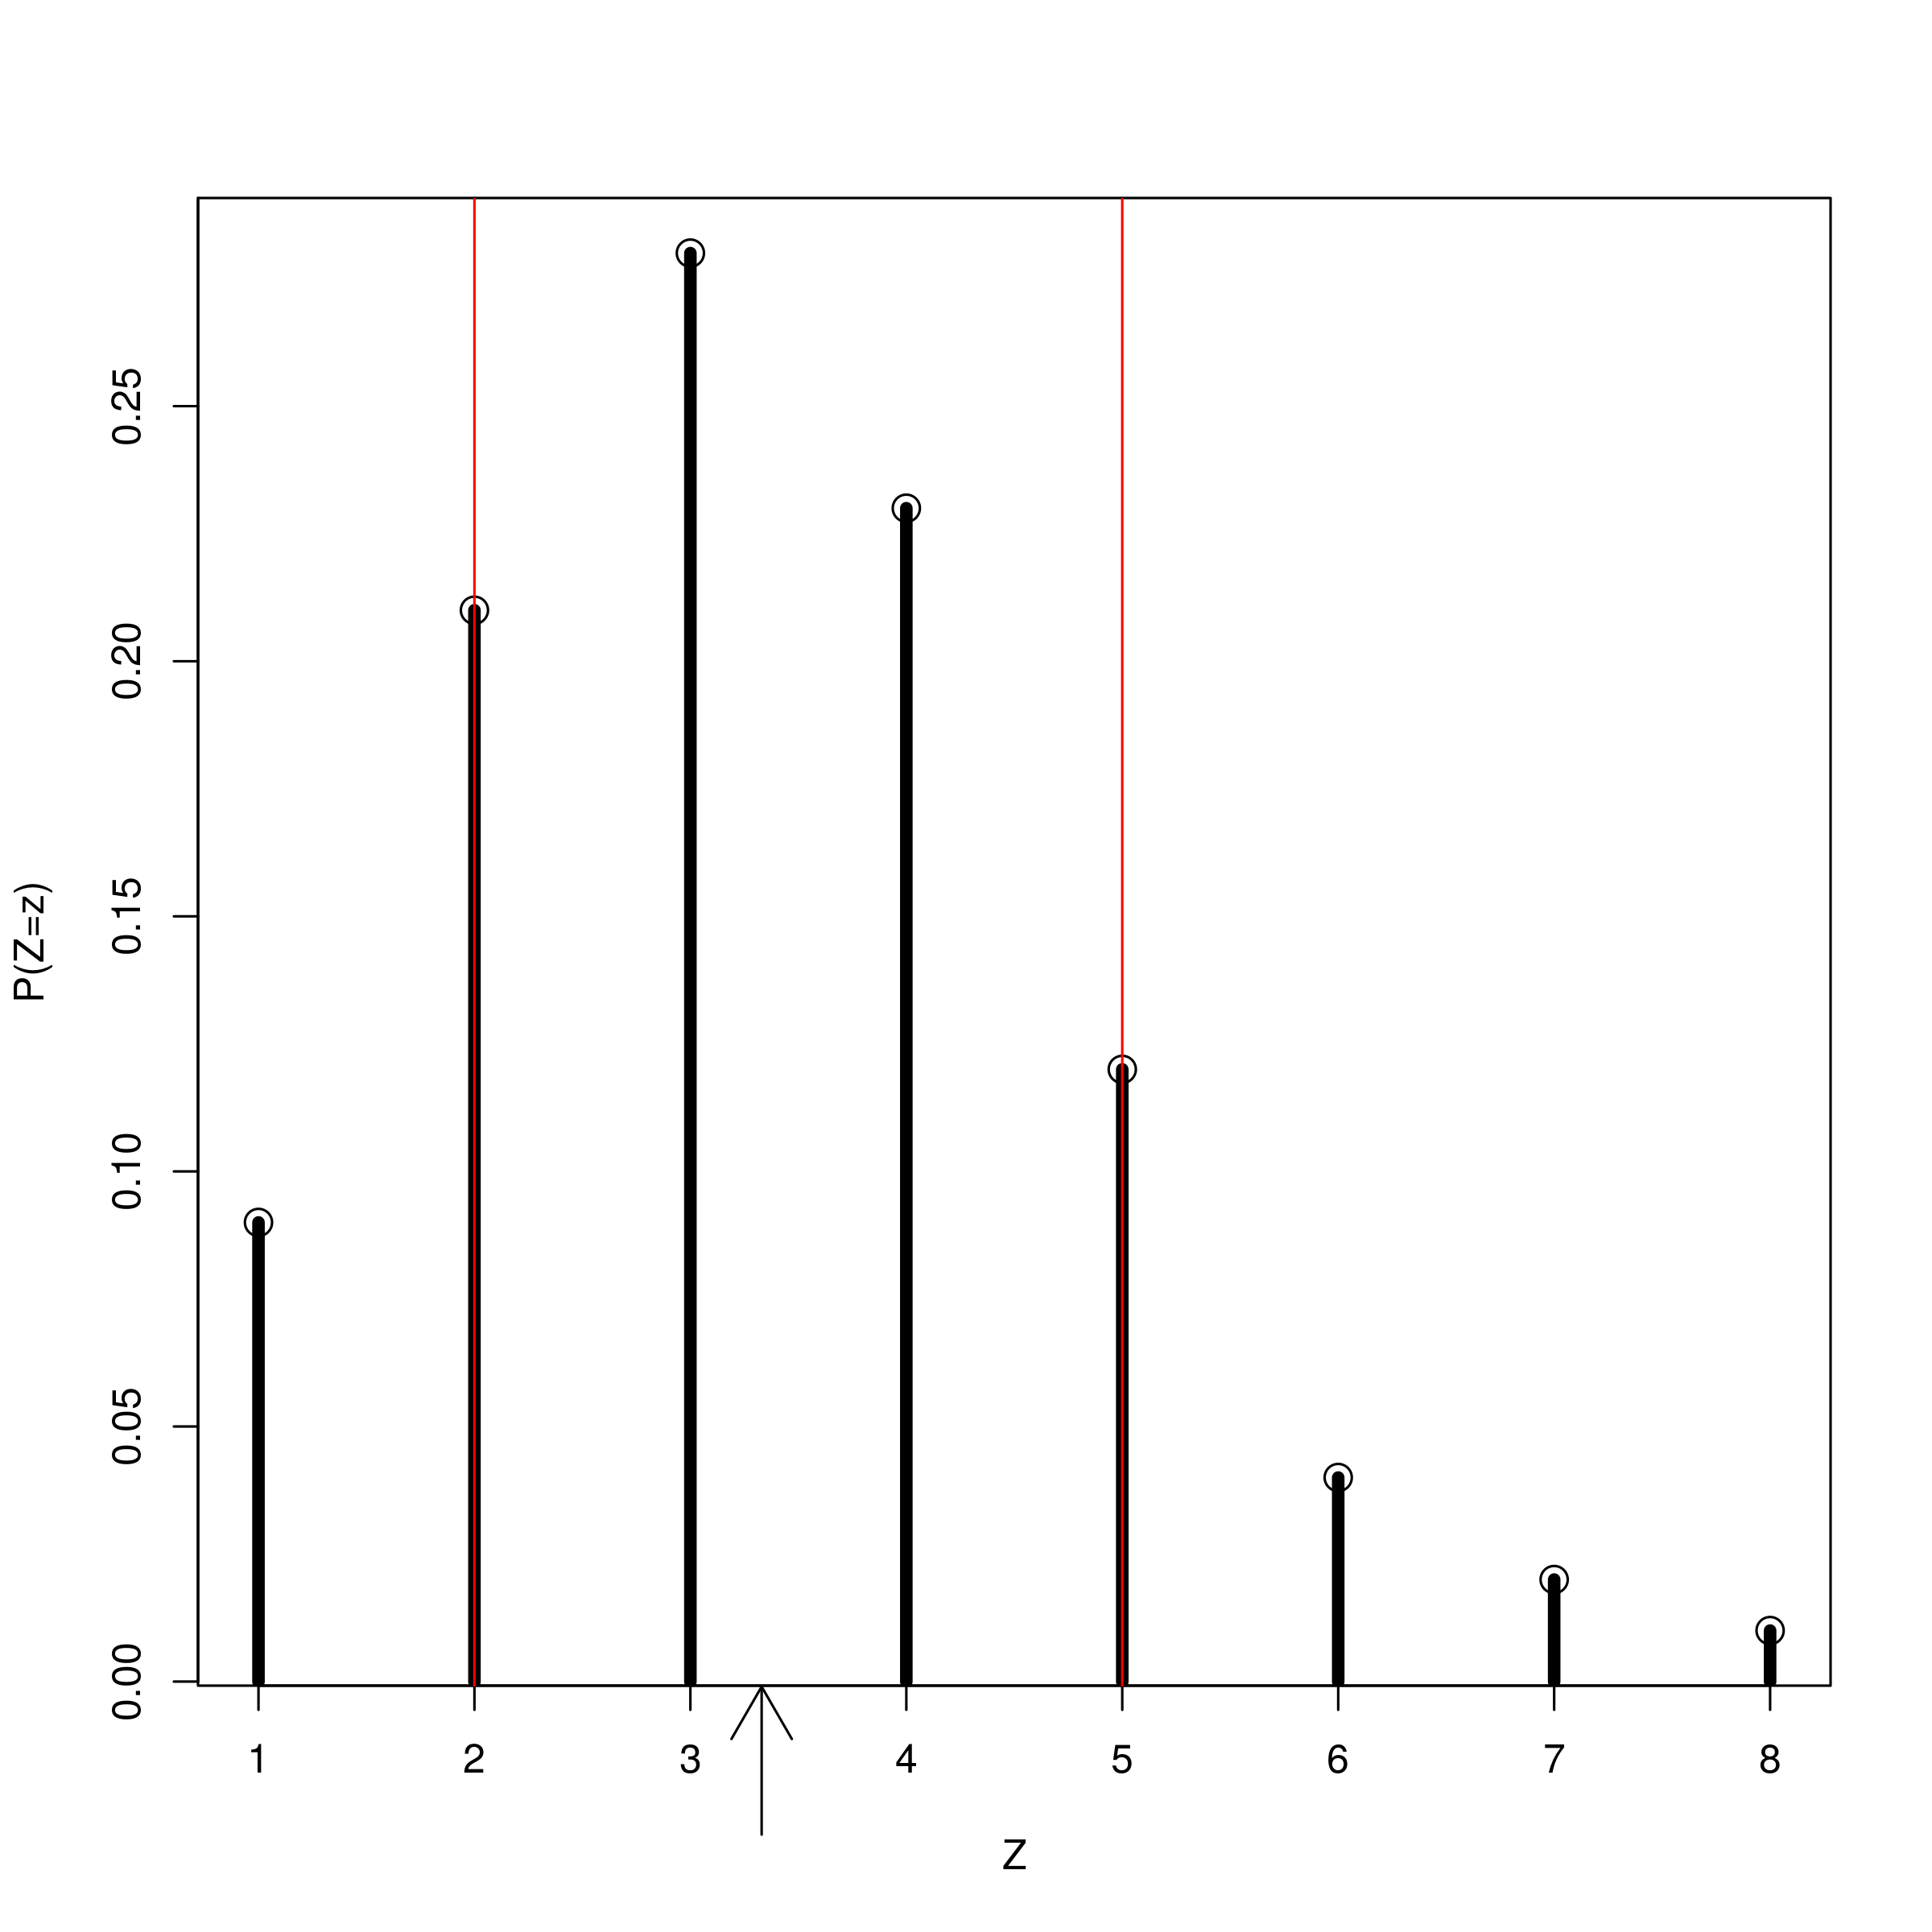
\includegraphics[scale=.4]{distribution.png}
\caption{Probability distribution of a random variable $Z$ with $ 8 $ possible values, given by $ P(Z = 1) = 0.09,  P(Z = 2) = 0.21, P(Z = 3) = 0.28, P(Z = 4) = 0.23, P(Z = 5) = 0.12, P(Z = 6) = 0.04, P(Z = 7) = 0.02$, and $ P(Z = 8) = 0.01$. The arrow indicates the expectation. This is a visualisation of 
the spike that we can plug underneath the centre of mass.}
\label{binomplot}
\end{figure}

\begin{figure}
\center
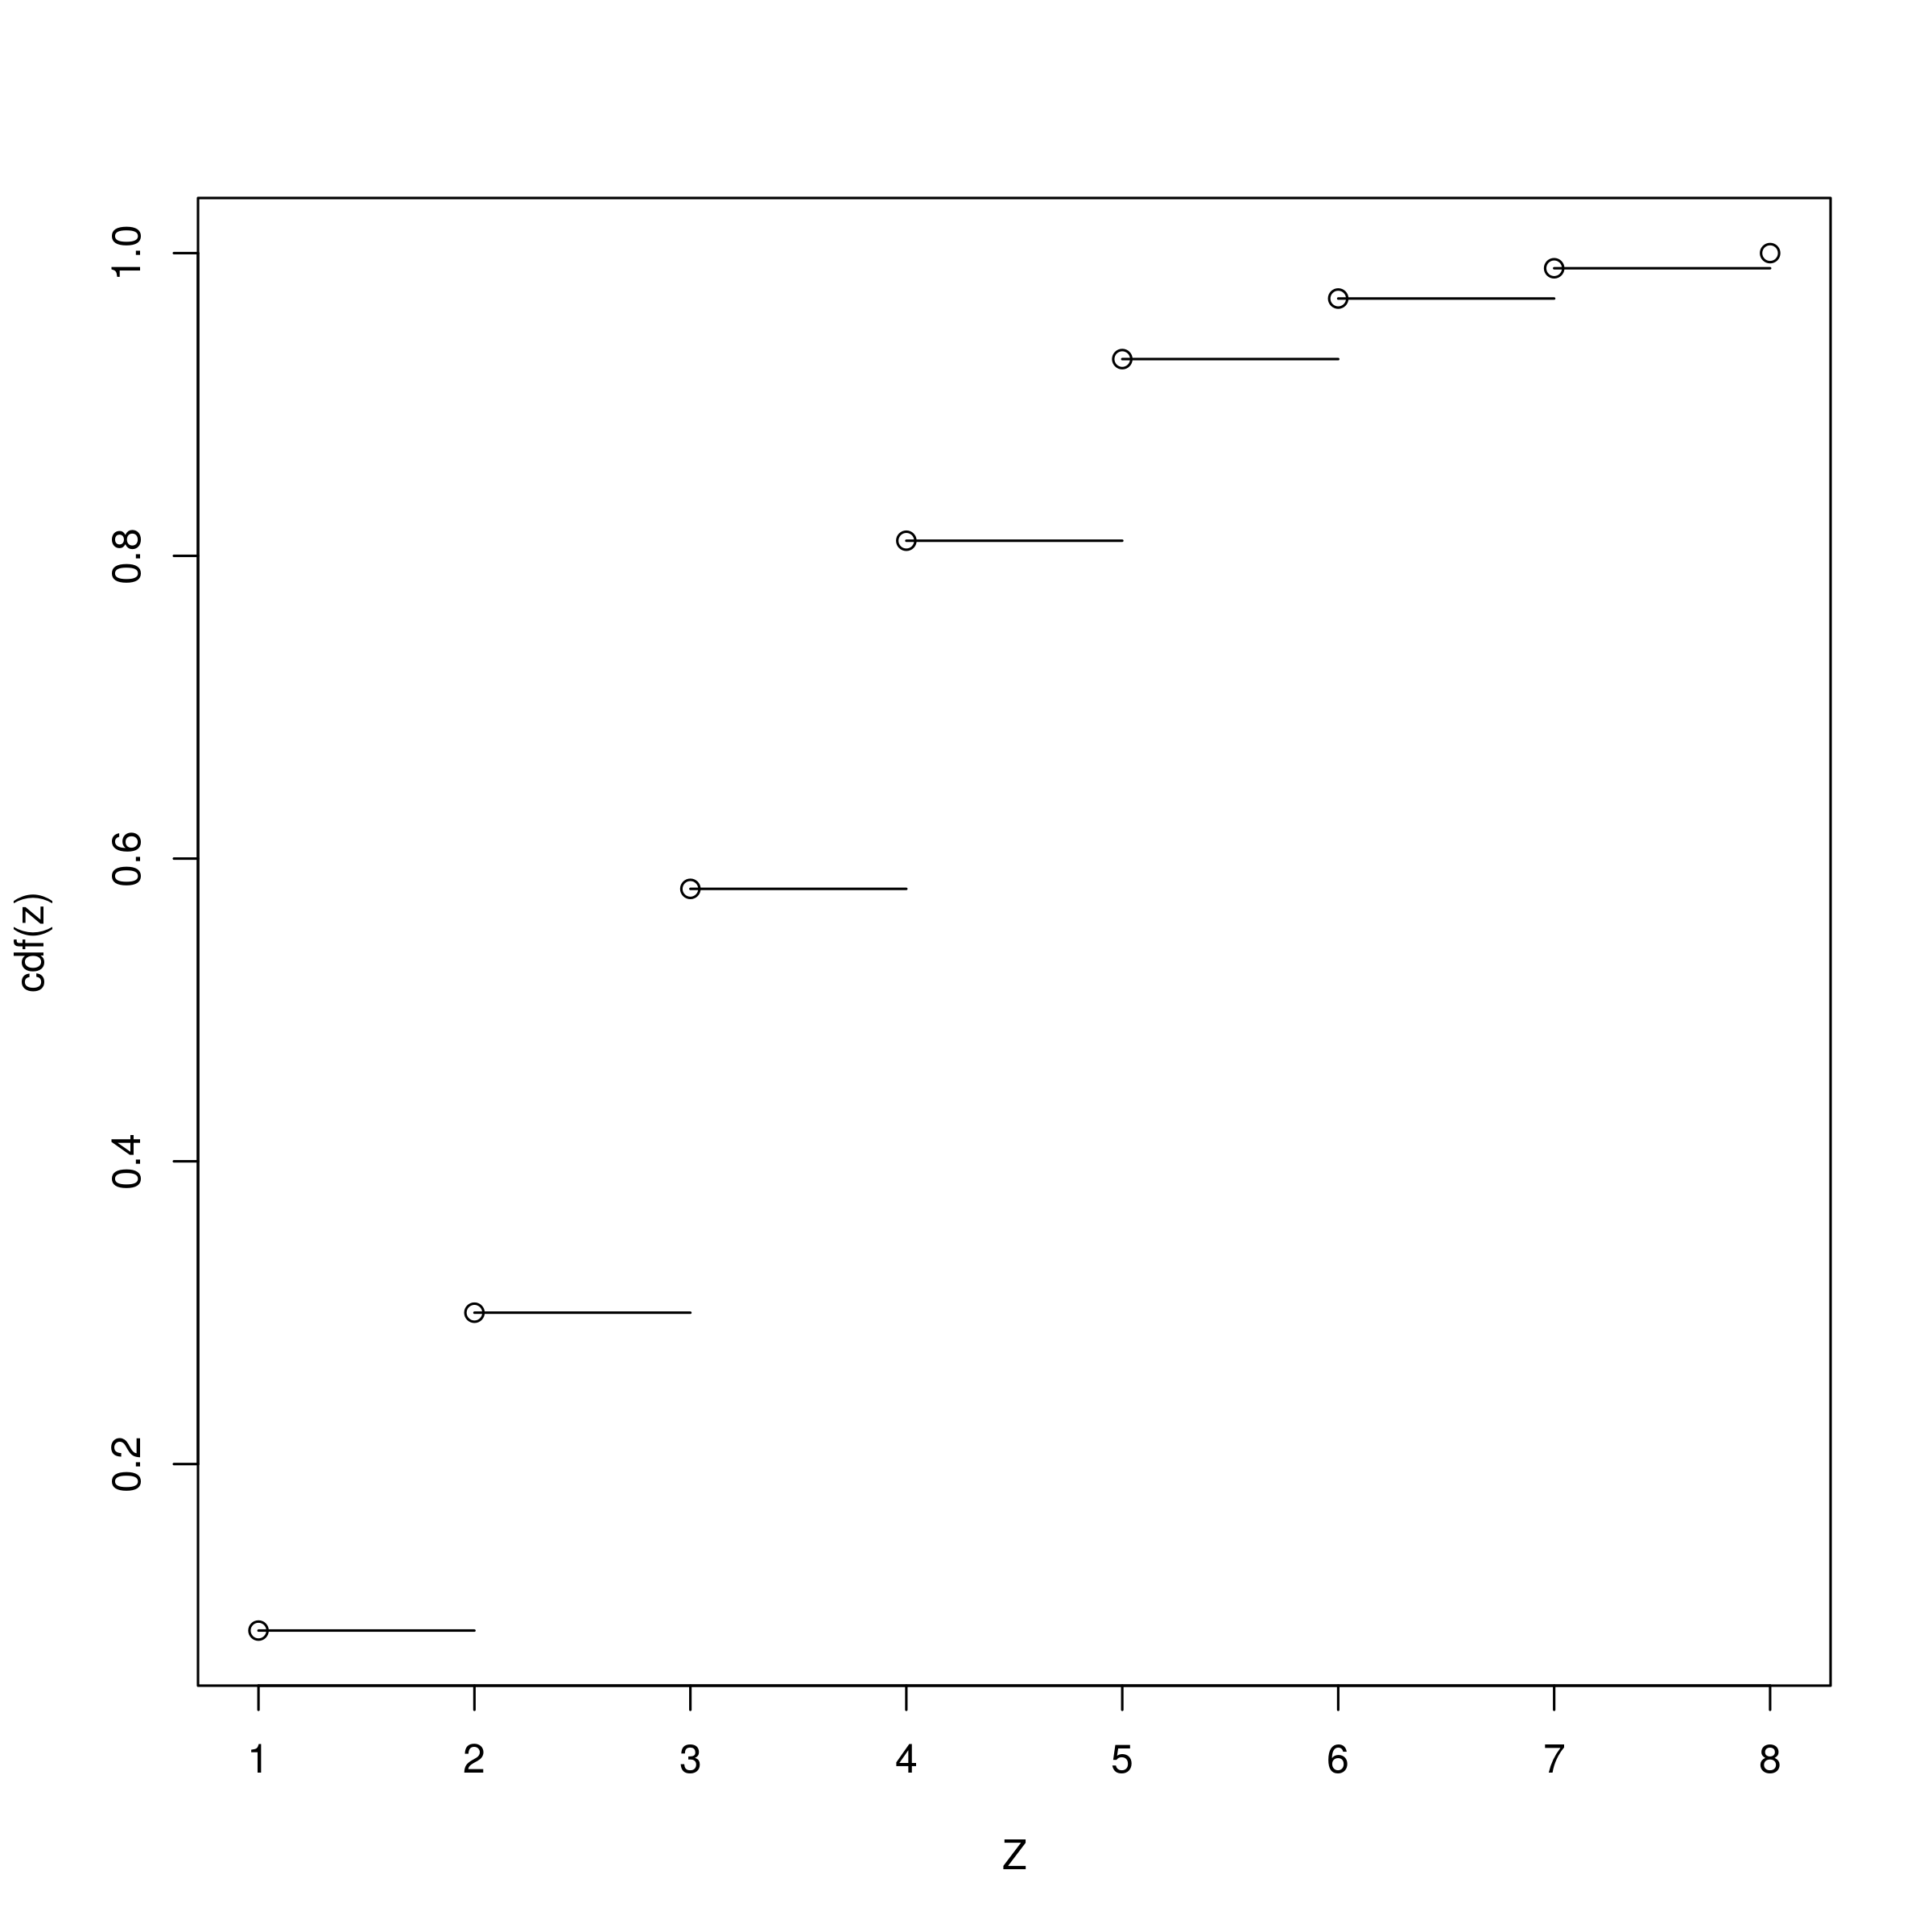
\includegraphics[scale=.4]{cdf.png}
\caption{Cumulative probability distribution of $ Z $. Observe that it stays constant in values that $ Z $ cannot take on. This cdf being discontinuous is an indicator
that the underlying probability distribution is discrete.}
\label{cdfPlot}
\end{figure}

To better understand how we can compute the probability that $ a \leq X \leq b $ for some real values $ a,b $ let us take a 
look at Figure~\ref{binomplot}. There we see a plot of the probability distribution of a random variable $ Z $. The red lines
indicate the interval that we are interested in. As a warm-up exercise, let us first compute $ P(Z \leq 2) $ and 
$ P(Z > 5) $. By looking at the plot we easily see which areas we need to consider, namely the bars to the left of 2
and to the right of 5. The height of the bars corresponds to their probability. 

We go on to compute the probability that $ Z $ is smaller or equal to 2 and that $ Z $ is bigger or equal to 5:

\begin{align}
P(Z \leq 2) =& P(Z=1) + P(Z=2) = 0.09 + 0.21 = 0.3 \\
P(Z > 5) =& P(Z=6) + P(Z=7) + P(Z=8) \\ 
=& 0.04 + 0.02 + 0.01 = 0.07 \nonumber
\end{align} 

It is straightforward to compute $ P(2 < Z \leq 5) $. If we again look at Figure~\ref{binomplot}, we see that this is
the area delimited by the red lines. Thus, $ P(Z \leq 5) $ will be an overestimate of this probability. The amount by
which it is an overestimate is exactly $ P(Z \leq 2) $. Thus we get $ P(2 < Z \leq 5) = P(Z \leq 5) - P(Z \leq 2) $.

\begin{Exercise}
We claim that you can compute $ P(2 < Z \leq 5) $ based on $ P(Z \leq 2) $ and $ P(Z > 5) $ from above. What result do
you get?
\end{Exercise}

In the case of discrete random variables, i.e.\ the ones that we are dealing with here, there is another function that is of great interest, namely the probability mass function.

\begin{Definition}[Probability mass function]
The \textbf{probability mass function (pmf)} of a random variable $ X $ is given by
$$ p(x) := P(X = x) $$
\end{Definition}

The pmf is notationally more convenient than the probability distribution but also less general. For example, the pmf does not
allow us to express that $ X $ falls in a range of values. In order to avoid confusion, we will mostly use $ X $'s 
probability distribution here. Be aware, however, that most papers that you are going to read in the future will use the pmf
instead. Regardless of whether we are using the probability distribution or the pmf, we will call the values in $ \mathbb{R} $
to which they assign positive probability, their support.

\begin{Definition}
The \textbf{support} of a random variable $ X $ is given by
$$ \supp(X) := \{x \in \mathbb{R} \mid P(X=x)>0 \} $$
\end{Definition}




\section{Expectation and Variance}

There are two major properties of probability distributions that are used to describe them. One is the center of mass, the point
at which the probability mass of the distribution is split into half. If you think of the support of $ P $ as a plank and 
of the probabilities as weights, then the center of mass is the point at which you could put an infinitely thin spike into the
plank from underneath such that the plank maintains perfect balance. In Figure~\ref{binomplot} this so-called expectation
is indicated by an arrow that can be interpreted as visualising the spike that we can plug underneath the probability plank.

\begin{Definition}[Expectation]
The \textbf{expectation} of a random variable $ X $ with respect to the distribution $ P $ is defined as
$$ \E[X] := \sum_{x \in \supp(X)} x P(X=x) \, . $$
\end{Definition}

\begin{Exercise}
Compute the expectation of the random variable $ Z $ from the previous section.
\end{Exercise}

It is important to point out that the expectation of a random variable is a real number  which does not need to in the support of $ X $. This is for example the case in Figure~\ref{binomplot} where the
expectation is fractional although all support values are integers.

The expectation comes with an interesting property that is called the \textbf{linearity of expectation}. Basically, whenever we multiply $ X $ with a constant $ a $, the expectation will also be scaled by that constant. Moreover, when we add a constant $ b $
to $ X $ the expectation will also increase/decrease by $ b $ (depending on whether $ b $ is positive or negative). Let us
prove that!

\begin{align}
\E[aX+b] &= \sum_{x \in \supp(X)} (ax+b) P(X=x) \\
&= a \!\! \sum_{x \in \supp(X)} x P(X=x) \; + \; b \!\!\!\! \sum_{x \in \supp(X)} P(X=x)\\
&= a \E(X) + b \label{sumToOne}
\end{align}

The equality in \eqref{sumToOne} follows from the fact that the sum of the probabilities of the support of a distribution is 1.
The linearity of expectation is extremely useful. Basically, if you know the expectation of a RV you also know the 
expectation of its multiples. Furthermore, by adding a constant, we basically shift each element in the support. However, this shifting
does not do anything surprising as the centre of mass shifts by the same amount.

We can actually take the expectation of any quantity, but it only has an effect on quantities that
can be cast as functions of $ X $. The expectation of a quantity that is constant with respect to $ X $ will just be that
quantity itself. More formally:
\begin{equation}
\E[b] = \sum_{x \in \supp(X)} b P(X=x) = b
\end{equation}

A class of functions of $ X $ that people are often interested in are
the moments. Moments are the powers of $ X $, so $ X $ itself is the
first moment, $ X^{2} $ is the second moment and so on. We will not
further discuss moments here, but it is useful to at least know what
they are in case you find the expression in a paper.

\medskip
After we have discussed the centre of mass, it is also interesting to look at how far the outcomes are spread around the average. Assume two random variables $ X $ and $ Y $ with
\begin{itemize}
\item $ P(X=-100) = 0.5 $; $ P(X=100) = 0.5 $
\item $ P(Y=-1000) = 0.5 $; $ P(Y=1000) = 0.5 $
\end{itemize}
The spread of $ Y $ is obviously going to be greater, although both have the same expectation. The quantity usually used to assess
the spread of a RV is the variance.

\begin{Definition}[Variance]
The variance of a RV $ X $ is given by
$$ var(X) := \E[\, (X - \E[X])^{2} \, ] \, .$$
\end{Definition}

The expression for $ var(X) $ is rather scary-looking but let us try to make sense of it. The inner part is the difference between
each value of the random variable and the expectation. Thus the outer expectation is just a weighted sum of differences between 
values in the support and the expectation. However, since values of $ X $ can be smaller or greater than the expectation, this
sum will be 0. Therefore we square it, leaving us with only positive values. In summary, the variance is the expectation
of the squared differences between the expectation and the values in the support of $ X $.

Computing the variance as an expectation can be cumbersome. We show how it can be done more efficiently.
\begin{align}
var(X) &= \E[\, (X - \E[X])^{2} \, ] \\
&= \sum_{x \in \supp(X)} P(X=x) (x - \E[X])^{2} \\
&= \sum_{x \in \supp(X)} P(X=x) (x^2 - 2x\E[X] + \E[X]^{2}) \\
&= \sum_{x \in \supp(X)} P(X=x)  x^{2} -  \!\!\!\!\! \sum_{x \in \supp(X)} \!\!\!\!\! P(X=x) 2x\E[X] + \E[X]^{2} \\
&= \E[X^{2}] -   2 \E[X]^{2} + \E[X]^{2}  \\
&= \E[X^{2}] - \E[X]^{2} \, . \label{variance}
\end{align}

For most intents and purposes we will use \eqref{variance} to compute the variance. 

% Also, from here on, we will generally drop the 
% subscript indicating the distribution of the the expectation in order to save ourselves some writing.

\begin{Exercise}
Compute the variance of the RV Z from the previous section.
\end{Exercise}

Although variance is not linear, we can still try to figure out what happens when we multiply a RV by a constant or add a constant to it.
\begin{align}
var(aX+b) &= \E[ (aX+b - \E[aX+b])^2 ] \\
&=\E[ (aX+b - a\E[X] - b)^2 ] \\
&=\E[ a^2 (X-\E[X])^2 ] \\
&= a^2 var(X)
\end{align}

\begin{Exercise}
Give an alternative proof of $var(aX+b) = a^2 var(X)$ by using $var(X)
= \E[X^{2}] - \E[X]^{2}$.
\end{Exercise}
% \begin{align}
% \E[(aX+b)^{2}] - (\E[aX+b])^{2} \\
% &= \E[(aX+b)^{2}] - (a\E[X]+b)^{2} \\
% &= \E[a^{2}X^{2} + 2abX + b^{2}] - a^{2}\E[X]^{2} - 2ab\E[X] - b^{2} \\
% &= a^{2}\E[X^{2}] + 2ab\E[X] + b^{2} - a^{2}\E[X]^{2} - 2ab\E[X] - b^{2} \\
% &= a^{2}\E[X^{2}] - a^{2}\E[X]^{2} = a^{2}var(X) \
% \end{align}

What we see that the variance is not affected by adding a constant to the RV. This makes sense, as constant additions just shift
the expectation. However, the relation of each individual value to the expectation is not affected by that operation. On the other hand,
when we multiply each value of the RV by a constant, the variance is scaled by the square of that constant. Again, this is not surprising.
Remember that we used squaring in our definition of the variance to turn all distances from the expectation into positive numbers.
If we multiply an RV by a constant $ a $, its spread will increase in both directions by a factor of $ a $. 
Since we again want only positive differences,
we better square that increased spread. This intuitively justifies the above equalities.



\section{Joint and conditional distributions}

Up to now, we have only looked at cases that could be treated with one random variable. Most interesting problems involve several RVs, however. We introduce the concept of jointly distributed random variables. What this means is that
there is a distribution over tuples of values, each from a different RV.

\begin{Definition}[Joint probability distribution]
Random variables $ X_{1}, \ldots, X_{n} $ (\textbf{abbreviated as $ X^{n}_{1} $}) 
are said to be \textbf{jointly distributed} with probability distribution $ P_{X_{1}^{n}} $ if
$$ P(X_{1}=x_{1}, \ldots, X_{n}=x_{n}) = \mathbb{P}(\, \{\omega \mid
X_{1}(\omega) = x_{1}, \ldots, X_{n}(\omega)=x_{n}\}\, ) \, . $$ 
\end{Definition}

From the above definition, we see that the random variables need to
share an underlying sample space. This also gives us more insight into
the real power of RVs: in applications, we usually do not care at all
about the underlying sample space but only about quantities
captured by the RVs. Therefore, we define a probability distribution over the
random variables of interest. Since by definition the distribution has
to fulfil conditions that allow us to interpret the distribution
as a probability measure on a probability space, we can use the distribution without worrying
about the underlying sample space.

Joint distributions are of particular interest because they make it possible to recover the probability distribution of each individual
RV as well as of smaller joint distributions. The process by which this recovery can be accomplished is known as \textbf{marginalization}. Say
we are given a joint distribution $ P_{XY} $. How can we determine the probability that $ X=x $? Our sample space is carved
up by the values that $ X $ and $ Y $ can take on. We are interested in the probability of the subset $ E = \{\omega|X(\omega)=x\} $.
Assuming that $ Y $ can take on $ n $ values $y_1,y_2,\ldots,y_n$, let us define $ F_{i} = \{\omega| Y(\omega) = y_{i}\} $ for $ 1 \leq i \leq n $.
Some (possibly all) of the $ F_{i} $ will overlap with $ E $. Thus we can partition $ E $ into $ E\cap F_{1}, \ldots, E \cap F_{n} $.
By countable additivity, we simply need to sum up the probabilities of these intersections. Observe that those probabilities correspond exactly to $ P(X=x,Y=y_{1}), \ldots, P(X=x,Y=y_{1}) $. Hence, we get to the following equality:

\begin{equation} \label{simpleMarginal}
P(X=x) = \overset{n}{\underset{i=1}{\sum}} P(X=x,Y=y_{i}) 
\end{equation}

If we set $ X = (Z_{1}, \ldots, Z_{m}) $, we can recover $ P_{Z_{1}^{m}} $ from $ P_{Z_{1}^{m}Y} $ in the same way. Likewise,
if we set $ Y = (Z_{1}, \ldots, Z_{m}) $ we get the generalization of \eqref{simpleMarginal}. We will assume that each $ Z_{j} $
can assume $ n_{j} $ values.

\begin{align}
P(X=x) = \overset{n_{1}}{\underset{j_{1}=1}{\sum}}\ldots \overset{n_{m}}{\underset{j_{m}=1}{\sum}} 
P(X=x,Z_{1}=z_{j_{1}}, \ldots, Z_{m}=z_{j_{m}})
\end{align}

For exercise purposes, it often helps to draw a joint probability table and do marginalization from there.

\begin{table}
\center
\begin{tabular}{|c|c|c|c|}
\hline
$X\backslash Y$	& 1		& 2		& 3		\\
\hline
1				& 0.15	& 0.08	& 0.07	\\
2				& 0.01	& 0.2	& 0.03	\\	
3				& 0.28	& 0.17	& 0.09	\\
\hline
\end{tabular}
\caption{Joint probability table for $ X $ and $ Y $.}
\label{jointTable}
\end{table}

\begin{Exercise}
Find the marginal distributions $ P_X $ and $ P_{Y} $ in table \ref{jointTable}.
\end{Exercise}

We have already seen how the joint probability of random variables links back the the probability space that underlies them.
This link makes it easy to import certain concepts that we have
gotten to know in previous chapters. In particular, we can define \textbf{conditional probability distributions}.

\begin{Definition}[Conditional probability distribution]
Let $X,Y$ be random variables with joint distribution $P_{XY}$. Let
$y$ be such that $P(Y=y)>0$. The probability of $ X = x $ conditioned on $ Y=y $ is given by
$$ P(X=x|Y=y) := \dfrac{P(X=x, Y=y)}{P(Y=y)} \, . $$
The conditional distribution of $X$ given $Y=y$ is denoted by $P_{X|Y=y}$.
\end{Definition} 

\begin{Exercise}
Compute the conditional probability distributions $ P_{X|Y=2} $ and $ P_{Y|X=1} $ from Table~\ref{jointTable}.
\end{Exercise}

Likewise, the concept of independence carries over to distributions.

\begin{Definition}[Independence of random variables]
Two random variables $ X,Y $ are independent (denoted by $ X \bot Y $)
if $P_{XY} = P_X P_Y$, i.e.\ $\forall x \in \supp(X), \forall y \in \supp(Y): P(X=x, Y=y) = P(X=x)P(Y=y) $.
\end{Definition}

As with events, independence is equivalent to $ P_{X|Y} = P_{X} $ (and
to $P_{Y|X}=P_Y$). Moreover, independence makes it much easier to calculate the expectation and variance of functions of jointly distributed random variables\footnote{Notice that the joint random variable $(X,Y)$ is not a \emph{real-valued} random variable anymore. Hence $\E[X,Y]$ and $var(X,Y$) are not defined. Rather, we can define a new (real-valued) random variable as $f(X,Y)$ for a function $f: \mathbb{R} \times \mathbb{R} \rightarrow \mathbb{R}$. and compute $\E[f(X,Y)]$ and $var(f(X,Y))$.}. For independent $X$ and $Y$, we have
\begin{align}
\E[XY] &= \sum_{x \in \supp(X)} \sum_{y \in \supp(Y)} P(X=x,Y=y) x y \\
&= \sum_{x \in \supp(X)} \sum_{y \in \supp(Y)} P(X=x)P(Y=y) x y \\
&= \sum_{x \in \supp(X)} P(X=x)x \sum_{y \in \supp(Y)}  P(Y=y) y \\
&= \E[X]\E[Y]
\end{align}

Similarly, it does not really make sense to talk about the variance of two random variables (at least not as one single
value). However, we can again compute the variance of functions. For addition, independence again makes our lives
much easier.

\begin{Exercise}
Show that for independent RVs $X$ and $Y$, we have that $ var(X + Y) =
var(X) + var(Y) $. Give an example of dependent $X$ and $Y$ with $ var(X + Y) \neq
var(X) + var(Y) $.
\end{Exercise}



\section{Three Important Distributions}

We will finish this chapter by introducing two extremely useful discrete distributions. They are very often used in
computer science to model the probability of bit strings and in linguistics and natural language processing to model
the probability of sentences. 

To get us started, let us consider coin tosses. When you toss a fair coin, the probability that it lands on heads is 0.5 and
so is the probability that it lands on tails. Let $ 1 $ stand for heads and $ 0 $ for tails in a random variable $ X $ 
modelling coin tosses. We can formalize this distribution as
\begin{equation*}
P(X=x) = 0.5^{x}\times 0.5^{1-x} = 0.5 \mbox{ for $x \in \{0,1\}$ .}
\end{equation*}

Notice though that not all coins are fair and that in general we want to allow for probabilities that are not equal. 
We will therefore introduce a parameter $ \theta $ that regulates the probability that we observe heads. In the
above equation, we set $ \theta = 0.5 $. What happens if we set $ \theta = 0.3 $?
\begin{equation}
P(X=x) = 0.3^{x} \times 0.7^{1-x} = 
\begin{cases}
0.3 & \mbox{ if $x=1$} \, , \\
0.7 & \mbox{ if $x=0$} \, .
\end{cases}
\end{equation}

Where did we get the 0.7 from? Well, we know that the coin has to land on either heads or tails. Thus, if the probability
to land on heads is $ 0.3 $ the probability to land on tails has to be $ 0.7 $. Moreover, we chose $ 1 $ as a stand-in for
landing on heads. As we would expect, $ X = 1 $ will return the $ 0.3 $ probability and $ X = 0 $ will return the probability of $ 0.7 $.

This leads to a general formulation where we do not specify the parameter $ \theta $ but leave it to be filled in. 
The resulting distribution, known as \textbf{Bernoulli distribution} (with parameter $ \theta $), is shown in Equation~\eqref{Bernoulli}.
\begin{equation}\label{Bernoulli}
P(X=x) = \theta^{x} \times (1 - \theta)^{1-x} =
\begin{cases}
\theta & \mbox{ if $x=1$} \, , \\
1-\theta & \mbox{ if $x=0$} \, .
\end{cases}
\end{equation}

The Bernoulli is defined for one coin flip, or more generally for the
drawing of a coloured ball from a (very large) urn containing balls
of exactly two colours (in proportion $\theta$ and $1-\theta$). What if we draw balls repeatedly with replacement? We will get a sequence of coloured balls. 
Say we draw $ n $ balls and repeat this procedure five times. Chances are that the five sequences will look rather different.
Thus, we can define a probability distribution over sequences of
coloured balls of length $ n $. This procedure can be described as a simple generalization
of the Bernoulli. Whereas in the Bernoulli we made one draw we make $
n $ draws. This yields a sequence $ x $ in which each position $ x_{i}, 1 \leq i \leq n $ is either $ 0 $ or $ 1 $.
\begin{equation}\label{Multinoulli}
P(X=x) = \theta^{\sum_i x_i} \times (1 - \theta)^{n-\sum_i x_i}
\end{equation}

The adjustment is rather small. We basically only introduce an extra parameter, namely the number of draws $ n $. 
However, there are two conditions for this distribution that we have not mentioned yet. First and foremost,
the repeated Bernoulli draws are assumed to be independent. That is, for each draw in the sequence it should not matter which colours you
have drawn so far and which ones you are still going to draw (as you
are drawing with replacement). More formally, if we encode each draw in the sequence as a random
variable, we postulate that these random variables are independent of each other. 

The second point is that we cannot assign a probability to any sequence that contains more balls of one colour than there are balls in total.
This is to say that we require that $ 0 \leq \underset{i=1}{\overset{n}{\sum}}x_{i} \leq n $ which is a reasonable restriction. 

It is also worth mentioning that in general the two values that the distributions in \eqref{Bernoulli} and \eqref{Multinoulli} range
over are generally referred to as success and failure where the success is usually encoded as $ 1 $ and the failure as $ 0 $. 

\begin{Exercise}
Use the distribution in Equation~\eqref{Multinoulli} with $ n = 10 $ and $ \theta = 0.8 $ to determine the probability of the sequence (0,0,1,1,0,1,1,1,0,1).
\end{Exercise}

Another interesting observation is that, since the value at each position in the sequence is independent of all others, all sequences with the same
number of successes and failures will have the same probability. At this point it is natural to ask for the probability to get \textit{any}
sequence with that amount of successes and failures. Say we are dealing with sequences of length $ n $ and wonder about the probability of 
obtaining a sequence with $ 0 \leq k \leq n $ successes. Then we simply need to sum up the probabilities of all sequences that contain $ k $ 
successes. But how many such sequences are there? In Chapter~1, we talked about how to choose a subset of $ k $ elements
out of $ n $. This is exactly the problem we are facing here. We want to know how many ways there are to choose $ k $ out of $ n $ positions
that we interpret as successes. This counting is done by the binomial co-efficient $ \binom{n}{k} $.

We can generalize the distribution from Equation~\eqref{Multinoulli} to a distribution that gives the probability of obtaining any sequence
with $ k $ successes. This distribution is known as the \textbf{binomial distribution} (with parameters $ n $ and $ \theta $).
\begin{equation}
P(X=k) = \binom{n}{k} \theta^{k} (1-\theta)^{n-k}
\end{equation}

The binomial is of crucial importance in many fields. For example in computer science, it is used to compute the probability of bit strings.
Other applications include the assessment of failure rates. Say you run a company and a customer asks you to supply $ k $ items within a week.
The capacity of your company allows you to produce at most $ n > k $ items during that week. At the same time you know that each item that you 
produce has a probability of being faulty. Obviously, you cannot sell faulty items to your customer. The Binomial distribution allows you to
compute the probability that you will be able to meet the customer's demand. Based on this calculation, you can evaluate whether or not it is reasonable to
accept the customer's order.

The third important distribution that we get to know today is the \textbf{multinomial distribution}. It is basically a generalization
of the binomial. A RV that is distributed according to the multinomial distribution can take on finitely many values. Let us say that
there are $ m $ such values. Furthermore let us assume that each value occurs $ c_{i} $ times in a sequence of length $ n $ where
$ 1 \leq i \leq n $ and $ \underset{i=1}{\overset{m}{\sum}}c_{i} = n $. Then the multinomial with parameters $ n $ and 
$ \theta_{1}, \ldots, \theta_{n} $ is given as 
\begin{equation}
P(X_{1}=c_{1}, \ldots, X_{m}=c_{m}) = \dfrac{n!}{\underset{i=1}{\overset{m}{\prod}}c_{i}!}~\underset{i=1}{\overset{m}{\prod}} \theta_{i}^{c_{i}}
\end{equation}

A further condition on the multinomial is that $ \underset{i=1}{\overset{m}{\sum}}\theta_{i} = 1 $. Just as with the binomial, we can
in principle infer (the last) $ \theta_{m} $ and $ c_{m} $ if we know the value of the other $ \theta_{i} $ and $ c_{i} $, $ 1 \leq i \leq (m-1) $. However, this would
clutter notation unnecessarily and we hence do not do it here. It is noteworthy, though, that because of this fact, the multinomial
has $ m-1 $ and not $ m $ $ \theta $-parameters (since $ \theta_{m} $ is determined by the other $ \theta_i $).

It is easy to see that the binomial is in fact just the special case
$m=2$ of the multinomial. Because of its general importance it is usually
considered a separate distribution though.

Let us finish this section by introducing some useful notation. When a RV is distributed according to some distribution, one often uses
the tilde($\sim$) to express this fact. If, for example, we have a random variable $ X $ that is distributed according to a binomial with $ n=100 $
and $ \theta = 0.5 $, many authors will write
$$ X \sim binom(100, 0.5) $$
Now that we know what it means for a random variable to be distributed according to some distribution, we can also clarify a question 
that was brought up in the beginning. What does sampling \textit{uniformly at random} mean? It just means that we are sampling from
a distribution that is the uniform distribution (all values in the support have the same probability). The \textit{random} comes from the fact that
we are sampling the values of a random variable. Just saying that some quantity is sampled at random is not enough. You should
always add which distribution underlies that randomness!


\section{The Negative Binomial Distribution$ ^{*} $}
Another interesting distribution that is well worth looking at is the negative binomial distribution. Suppose we do repeated independent Bernoulli trials and we wonder
how many trials it will take until we have observed $ k > 0 $ successes. To answer this question, we would like to assign a probability to each integer $ t \geq k $ which 
can be interpreted as the probability that we will take $ t $ trials until we have obtained the desired number of successes. Notice that for each $ t $, we can infer
the number of failures as $ f = t - k $.

To approach this problem, let us start out from the simplest case where we are only waiting for one success. In that case, our sequence of trials ends in a success,
which is also the only success in the sequence. Thus the sequence contains $ f = t-1 $ failures. The success probability of a Bernoulli trial is $ \theta $, as usual.
Then the associated probability distribution for $ T $ with parameters $ \theta $ and $ k=1 $ is
\begin{equation} \label{negBernoulli}
P(T=t) = \theta^{1} (1-\theta)^{t-1}
\end{equation}

Notice that if $ k=1 $ there is only one sequence of size $ t $ that ends in a success. If we let $ k>1 $, there are more sequences of length $ y $ that end in a success 
and contain $ k $ successes in total. The probability for any such sequence can easily be calculated by generalising Equation~\eqref{negBernoulli}.
\begin{equation}
P(T=t) = \theta^{k} (1-\theta)^{t-k}
\end{equation}

As with the Binomial, we now have to add up the probabilities of all sequences of length $ t $ that contain exactly $ k $ successes \textit{and end in a success}. The
last condition is what separates the negative Binomial from the Binomial distribution. We first observe that the position of the last success is fixed. This means
we are left with $ k-1 $ which we can assign to different positions. In total there are $ t-1 $ positions that we can assign. Thus we have to choose $ k-1 $ out
of $ t-1 $ position over which to distribute the remaining $ k-1 $ successes. Thus, we conclude that there are $ \binom{t-1}{k-1} $ sequences of length $ t $ that
contain $ k $ successes, one of which occurs in the last position of the sequence. This is allows us to define the negative Binomial distribution with parameters 
$ \theta $ and $ k $ as
\begin{equation}
P(T=t) = \binom{t-1}{k-1} \theta^{k} (1-\theta)^{t-k}
\end{equation}
where $ t \in \mathbb{N}, t > k $.

Many authors use the notation $ X \sim nbinom(\theta, k) $ to state that the RV $ X $ is distributed according to a negative Binomial distribution.



%%% Local Variables:
%%% mode: latex
%%% TeX-master: "chapter3"
%%% End:


\setcounter{chapter}{3}
\chapter{Bayes' rule and its applications}

\section{The chain rule}

This chapter is going to focus on how to re-write joint and conditional probabilities. When we turn to statistics later on, it will
turn out that it is often hard to define a joint distribution over many variables. Likewise, it can be hard to calculate 
the probability distribution of a RV $ X $ conditioned on a RV $ Y $ but it may be much easier to find the distribution of $ Y $
conditioned on $ X $. In this chapter we are essentially trying to find simpler expressions for distributions that may be hard to
compute.

The first general method for simplifying a joint distribution is known as the \textbf{chain rule}. \chris{skip? We could actually have introduced
the chain rule much earlier, when talking about the probability of events. However, we chose not to do so as it would have 
cluttered the presentation. Moreover, we only need the chain rule now.} For completeness' sake, we are going to formulate the chain rule first for events and then for random variables.

\begin{Theorem}{\textbf{(Chain rule)}} \label{thm:chain}
The joint probability of events $ E_{1}, \ldots, E_{n} $ can be factorised as
$$ \mathbb{P}(E_{1}, \ldots, E_{n}) = \mathbb{P}(E_{1}) \times \mathbb{P}(E_{2}|E_{1}) \times \ldots \times \mathbb{P}(E_{n}|E_{1}, \ldots, E_{n-1}) $$
\end{Theorem} 
Recall from Definition~\ref{def:jointprob} the notation $\mathbb{P}(E_1,E_2) = \mathbb{P}(E_1 \cap E_2)$ for denoting the probability that both events $E_1$ and $E_2$ occur. There are a couple of things to note about the chain rule: First of all, the numbering of the events is arbitrary. That means that it does not matter in which
order we decompose the joint probability. We could just as well start with any $ E_{i} $ for $ 1 \leq i \leq n $. Second we used the 
word \textit{factorise}. This simply means that we decompose any expression (in this case a joint probability) into a product. Products are
nice in that we can arrange them in any order that we like (i.e.\ they commute). Moreover, products make a lot of calculations easier, as we will
see later.

Let us go ahead and actually prove the chain rule. 
\paragraph{Proof of Theorem~\ref{thm:chain}} We are going to do so inductively and choose $ \mathbb{P}(E_{1}, E_{2}) $ as our
base case. Then we simply employ the definition of conditional probability to get
\begin{equation}
\mathbb{P}(E_{1}, E_{2}) = \mathbb{P}(E_{1}) \times \dfrac{\mathbb{P}(E_{1}, E_{2})}{\mathbb{P}(E_{1})} = \mathbb{P}(E_{1}) \times \mathbb{P}(E_{2}|E_{1})
\end{equation}

Let us assume that the chain rule holds for events $ E_{1}, \ldots, E_{n-1} $. We will abbreviate them as $ E_{1}^{n-1} $. Then we get
\begin{equation}
\mathbb{P}(E_{1}^{n-1}, E_{n}) = \mathbb{P}(E_{1}^{n-1}) \times \dfrac{\mathbb{P}(E_{1}^{n-1}, E_{n})}{\mathbb{P}(E_{1}^{n-1})} 
= \mathbb{P}(E_{1}^{n-1}) \times \mathbb{P}(E_{n}|E_{1}^{n-1})
\end{equation}

Since $ \mathbb{P}(E_{1}^{n-1}) $ factorises according to the chain
rule by our induction hypothesis, we have completed the proof.
$ \square $\bigskip

The chain rule can make our lives even simpler if we have independent events. Assume we want to compute the joint probability of 3 events 
$ E_{1},E_{2},E_{3} $ and we also know that $ E_{1} \bot E_{2} $. In this case our factorisation becomes \eqref{simpleFactor} where
the first equality follows from the chain rule and the second equality follows from independence between $ E_{1} $ and $ E_{2} $.
\begin{align} \label{simpleFactor}
\mathbb{P}(E_{1}, E_{2}, E_{3}) &= \mathbb{P}(E_{1}) \times \mathbb{P}(E_{2}|E_{1}) \times \mathbb{P}(E_{3}|E_{1},E_{2}) \\
&= \mathbb{P}(E_{1}) \times \mathbb{P}(E_{2}) \times \mathbb{P}(E_{3}|E_{1},E_{2}) \nonumber
\end{align}

We can now state the chain rule for random variables. There are two ways you can go about proving it. Either you 
calculate the probability of a specific setting of the variables or you just do the proof based on the distributions of the RVs.
So in the first case you would have to prove that
\begin{align*}
\forall x_1,\ldots,x_n: &P(X_{1} = x_{1}, \ldots, X_{n} = x_{n}) \\
&= P(X_{1} = x_{1}) \times \ldots \times P(X_{n} = x_{n}|X_{1}=x_{1}, \ldots, X_{n-1} = x_{n-1})
\end{align*}
whereas in the second case you would simply prove that
\begin{align*}
P_{X_{1}^{n}} = \overset{n}{\underset{i=1}{\sum}}P_{X_{i}|X_{1}^{i-1}}
\end{align*}

Incidentally, we also introduce a very short notation for the chain rule above. Note that it is not quite correct, since if
$ i = 1 $ we would be conditioning on $ X_{0} $. That is not to bad however, since we can always define ourselves a constant variable $ X_{0} $ that does not affect the distribution. Moreover, this notation is really just meant to be convenient, so you should just accept it as is when you encounter it in papers.

\begin{Exercise}
Prove the chain rule for random variables. The proof is totally analogous to the one give for events.
\end{Exercise}

\begin{Exercise}
Let $X_0$ be a constant RV, i.e.\ there exists $c \in \mathbb{R}$ such that $P(X_0 = c)=1$. 
Prove that $X_0$ is independent of any set of other random variables $X_1,\ldots,X_n$.
\end{Exercise}

\section{Bayes' rule}

In this section we are going to prove \textbf{Bayes' rule}. The rule follows directly from the chain rule.
The proof is really simple and thus of no great interest in and by itself. The consequences of Bayes' rule
are huge however. It will basically allow us to invert a conditional probability distribution. You may rightfully
ask: what's the deal? Well, as we said in the beginning, it may be hard to compute a conditional distribution in one
direction but much easier to compute it in the other direction. On top of that, Bayes' rule opens up a whole range of new possibilities. We will discuss those as we proceed in this chapter.
\begin{Theorem}{\textbf{(Bayes' rule)}}
The probability distribution of a random variable $ X $ given a random variable $ Y $ can be computed as
$$ P_{X|Y} = \dfrac{P_{Y|X}P_{X}}{P_{Y}} $$
\end{Theorem}

And here comes the proof:
\begin{equation}
P_{X|Y} = \dfrac{P_{XY}}{P_{Y}} = \dfrac{P_{Y|X}P_{X}}{P_{Y}} \, . \qquad  \square
\end{equation}

That was the proof! Considering how simple it was, it will be surprising to see what kind of benefits we can get out
of Bayes' rule. To get us started, let us introduce some terminology. In particular, each of the terms
in Bayes' rule has a specific name. You should really learn these names by heart as they crop up all over the place.

$$ \mathit{posterior} = \dfrac{\mathit{likelihood} \times \mathit{prior}}{\mathit{marginal~likelihood}} $$

The posterior is what we get after we have completed the computation. However, its name is related to the prior.
The prior is just the probability that we would place on $ P(X=x) $ \textit{a priori}. Therefore $ P_{X} $
is also known as the prior distribution. When we multiply the prior by the likelihood we get a new distribution
over $ X $ that is conditioned on $ Y $ \chris{after multiplication, we get the joint distribution of X and Y??}. This is the distribution that we place on $ X $ \textit{a posteriori}, i.e.
after having taken into account information about $ X $ that we may get from knowing the value of $ Y $. The marginal
likelihood of $ Y $ is simply needed to normalize the expression to a probability distribution (i.e. to make sure that
it sums to one). Why is it called marginal likelihood? The reason for this is how you can compute it. Recall that when
we are given a joint distribution $ P_{XY} $, we can obtain the distribution
$ P_{Y} $ by simply marginalizing over $ X $.
\begin{equation}
P(Y=y) = \sum_{x \in \supp(X)}P(X=x, Y=y)
\end{equation}

In addition to that, the chain rule allows us to factorise the joint probability. Thus we get
\begin{equation}
P(Y=y) = \sum_{x \in \supp(X)} P(Y=y|X=x) \times P(X=x)
\end{equation}

If you think that this looks an awful lot like the enumerator of Bayes' rule then you are exactly on the right track.
Essentially, we are just summing over all possible denominators (with respect to $ X $). Let us make this more
concrete with an example. Assume that we are given two coins. One of them is fair, meaning that it is equally probable
to come up heads or tails. The other coin is biased towards tails and we happen to know that its probability to come up
heads is only $ 0.3 $. Which coin is flipped is captured by a random variable $ X $ that takes on the value 0 if the
fair coin is used and the value 1 if the biased coin is used. We have no idea which coin is going to be tossed, it could
be either one. Therefore we set our prior to $ P(X=0) = P(X=1) = 0.5 $.

We flip the chosen coin 10 times and obtain 8 heads. The number of heads obtained during the 10 tosses is going
to be encoded by $ Y $. Since all tosses are independent of each other, $ Y $ will
follow a binomial distribution. For each of the two coins we also know the parameter of the binomial distribution.
For the fair coin it is $ \theta = 0.5 $ and for the biased coin it is $ \theta = 0.3 $. Let us compute each of the
enumerators separately.
\begin{align}
P(Y=8|X=0) \times P(X=0) &= \binom{10}{8} 0.5^8 (1-0.5)^2 \times 0.5 = 0.02195 \label{bayes1}\\
P(Y=8|X=1) \times P(X=1) &= \binom{10}{8} 0.3^8 (1-0.3)^2 \times 0.5 = 0.0007 \label{bayes2}
\end{align}
Remember that $ Y \sim binom(10,\theta) $ and that $ \theta=0.5 $ if $ X=0 $ and $ \theta=0.3 $ if $ X=1 $. 

All that is left do is to compute the marginal likelihood of $ Y $. Luckily for us, $ X $ only assumes two
values, so we only need to add up \eqref{bayes1} and \eqref{bayes2}.
\begin{align}
P(Y=8) = &P(Y=8|X=0) \times P(X=0) \\
&+ P(Y=8|X=1) \times P(X=1) = 0.02265 \nonumber
\end{align}

And finally we can apply Bayes' rule to compute the posterior probabilities of $ X $.
\begin{align}
P(X=0|Y=8) &= \dfrac{P(Y=8|X=0) \times P(X=0)}{P(Y=8)} \\
&= \dfrac{0.2195}{0.02265} = 0.969 \nonumber \\
P(X=1|Y=8) &= \dfrac{P(Y=8|X=1) \times P(X=1)}{P(Y=8)} \\
&= \dfrac{0.0005}{0.02265} = 0.031 \nonumber \\
\end{align}

There is a probability of $ 0.969 $ that the fair coin has been tossed when a sequence with eight heads is
generated and only a probability of $ 0.031 $ that the biased coin was tossed. Obviously, the probability of the fair 
coin is much higher. But how much higher? We can take the ratio of the two probabilities. This gives us 
$ \nicefrac{0.969}{0.031} \approx 31 $. We can conclude that the fair coin is 31 times more likely to have generated the sequence with
8 heads than the biased coin. But wait a second, can we maybe find this ratio somewhere else? It turns out that 
the ratio of the likelihoods is the same! That is $ \nicefrac{0.0439}{0.0014} \approx 31 $.

We started out by assuming that both coins were equally likely to be used. However, we then observed a sequence of 10 tosses, 8 of 
which were heads and that made it 31 times more likely that the fair coin was used. What if the priors had not been equal?
Actually, there is a more general story: While calculating the actual probabilities involves a lot of number crunching, just telling whether or not an observation will make one or the other event more likely is not too hard. [For the rest of this chapter, we assume that we only condition on events with non-zero probabilities such as $P(Y=y)>0$ so that we are never dividing by 0].
\begin{align*}
\frac{P(X=x_{1}|Y=y)}{P(X=x_{2}|Y=y)} &= \frac{\dfrac{P(Y=y|X=x_{1})P(X=x_{1})}{P(Y=y)}}{\dfrac{P(Y=y|X=x_{2})P(X=x_{2})}{P(Y=y)}} \\[1em]
&= \frac{P(Y=y|X=x_{1})P(X=x_{1})}{P(Y=y|X=x_{2})P(X=x_{2})}
\end{align*}

From the above equalities, we see that the ratio of the posterior probabilities is determined by the ratio of the likelihood times the
prior. In our coin example, the priors were the same so it was only the likelihood that mattered. If the ratio of any of the above
terms is greater than 1, the posterior will change in favour of $ X=x_{1} $. If the ratio is smaller than 1 the posterior changes
in favour of $ X=x_{2} $. If the ratio is exactly 1, nothing happens\chris{what do you mean by ``nothing happens''???}. 

Notice that in general, although our observations may shift the posterior in favour of $ X=x_{2} $, say, this shift does not necessarily imply that 
$ P(X=x_{2}|Y=y) $ will be greater than $ P(X=x_{1}|Y=y) $. The condition that $ P(X=x_{2}|Y=y) $ is bigger than  $ P(X=x_{1}|Y=y) $ can be rewritten as follows
\begin{align*}
P(X=x_{1}|Y=y) &< P(X=x_{2}|Y=y)  &\Leftrightarrow \\
\dfrac{P(Y=y|X=x_{1})P(X=x_{1})}{P(Y=y)} &< \dfrac{P(Y=y|X=x_{2})P(X=x_{2})}{P(Y=y)} &\Leftrightarrow \\
P(Y=y|X=x_{1})P(X=x_{1}) &< P(Y=y|X=x_{2})P(X=x_{2}) &\Leftrightarrow \\
\dfrac{P(Y=y|X=x_{1})}{P(Y=y|X=x_{2})} &< \dfrac{P(X=x_{2})}{P(X=x_{1})}
\end{align*} 

The last line is of particular interest as it elucidates the relationship between the prior and the likelihood. Only if the likelihood
ratio for $ X=x_{1} $ over $ X=x_{2} $ is smaller than the reversed prior ratio will the posterior probability of $ X=x_{2} $
be greater than that of $ X=x_{1} $. This means that if we have strongly asymmetric priors (like $ P(X=x_{1}) = 0.9 $
and $ P(X=x_{2}) = 0.1 $), the likelihood needs to discriminate very well between the two cases in order to tip the scale in
favour of $ X=x_{2} $. In that sense the prior and the likelihood can be seen as battling forces whose equilibrium gives us 
the posterior.

But enough theory about Bayes' rule, it is about time you apply it! To that end, we present you an exercise that is, in some variation,
contained in virtually every textbook on probability theory, statistics or machine learning. Have fun with it!

\begin{Exercise}
A random person walks into the doctor's office to be tested for a particular disease. The disease can be fatal if not treated. However,
successful treatment is possible if the disease is discovered early enough. It is commonly known that the disease occurs in 1 out
of 1000 people of the country's population. The doctor will administer a test that with a probability of 99\% returns a positive results
if the patient does indeed have the disease. At the same time, the test also returns a positive result in 5\% of the cases where the
patient does not have the disease. After the test has been administered to the patient in question, it returns a positive result.
What is the probability that the patient is infected with the disease? 
\\
Proceed as follows:
\begin{enumerate}
\item Write down a guess for what you think the probability might be (do not consider any math at this point).
\item Calculate that probability.
\item Check whether there is a considerable difference between your initial guess and the calculated probability. Go on to examine
how the different factors have influenced the probability of the patient having the disease.
\end{enumerate}
\end{Exercise}

Let us finish up this section with some more notation. In many applications of Bayes' rule we only want to know which outcome is
the most likely, without worrying too much about the actual probabilities. Likewise, there is a range of situations where we
just want to assign a score to outcomes and do not demand this score to be a probability. Throughout this chapter,
we have repeatedly encountered the following phenomenon: In order to rank the values of an RV according to their probabilities, we do not necessarily need to compute the marginal likelihood since it cancels in all these comparisons anyway. Therefore, you will often see authors stating that
\begin{equation} \label{proportionality}
P(X=x|Y=y) \propto P(Y=y|X=x)P(X=x)
\end{equation}

This equation reads as ``the posterior is proportional to the product of the likelihood and the prior''. In general, if we have two quantities
$ a $ and $ b $, then by $ a \propto b $ we mean that there is some constant $ C \in \mathbb{R} $ such that $ a = cB $. Notice
that the probability distribution is a function and hence we require $ C $ to be the same across the domain of that function (that
is $ C $ should be the same for all values of $ X $).

\begin{Exercise}
What is the value of $ C $ in Equation~\eqref{proportionality}?
\end{Exercise}



\section{Na\"ive Bayes}
In this section, we introduce a rather crude application of Bayes's rule which is surprisingly successful nonetheless.
Assume that instead of one random variable we are observing a sequence of random variables. Thus our problem is the following:
\begin{equation}
P(Y=y|X_{1}^{n}=x_{1}^{n}) \propto P(X_{1}^{n}=x_{1}^{n}|Y=y) \times P(Y=y) 
\end{equation}

By the chain rule we can decompose the right-hand side into
\begin{align}
P(Y=y|X_{1}^{n}=x_{1}^{n})
\propto &P(X_{1}=x_{1}|Y=y) \times \ldots \nonumber \\
&\times P(X_{n}=x_{n}|Y=y,X_{1}^{n-1}=x_1^{n-1}) \times P(Y=y) \nonumber
\end{align}

We are now going to introduce the aforementioned crudeness into the model by assuming that all $ X_1,\ldots,X_n$ are conditionally independent given $ Y $. Notice that
this is just an assumption that we are making without justification. In fact, it is very likely wrong. However, it makes our
live much easier because we only have to deal with very simple terms of the form $ P(X_{i}=x_{i}|Y=y) $. Because of the
crudeness of our assumptions, this probabilistic model is known as \textbf{na\"ive Bayes} (sometimes also 
stupid Bayes).

\begin{Definition}
A na\"ive Bayes model is a probabilistic model that assumes
$$ P_{Y|X_{1}^{n}} \propto P_Y P_{X_{1}|Y} P_{X_{2}|Y} \cdots P_{X_{n}|Y} $$
\end{Definition}
Once we know all the component distributions $P_{X_i|Y}$, calculating the result is pretty straightforward. 

In order to illustrate how na\"ive Bayes works we are going to employ one of its showcase applications where it indeed had
a lot of success in real life. The application we are talking about is text classification. The task is the following: you
are given some documents and for each of the documents you have to assign a label signifying its class. What you consider
a class depends on your actual application setting, but usually classes are broad categories, such as legal texts, medical
texts etc. If you manage to succeed at this task, you can accomplish a lot of things automatically that required humans before. For example, you could tag online news with their relevant categories and people who are interested in
a particular category will then have an easier time finding the news related to that category. Crucially, since you will
write a computer program that does the classification for you, you will not need to read any of the texts yourself. This automation will obviously allow you to classify huge quantities of text in a very short amount of time.

\begin{Exercise}
A collection of text (or any other kind of data for that matter) is often called a \textbf{corpus}. Here we are going to
use a toy corpus. The corpus just consists of two sentences and we assume that each sentence is its own document.
Your task is to classify these two documents correctly and report the posterior probability for the correct label. 
The categories that you can label the documents with are
finance (0), medicine (1) or law (2). You can find the corpus (the pmfs of the distributions) below. For simplicity, we are not going to distinguish between lower and upper case words (this is actually common practice). For better 
readability, we are also using the actual words instead of their numerical encodings as values for the random 
variables. Just remind yourselves that those words are real numbers in reality.
\end{Exercise}

\textbf{The corpus:}
\begin{itemize}
\item evidence ruled irrelevant or inadmissible shall not be considered by the chamber.
\item that is probably what investors who poured \$90 billion in european equity funds this year are hoping for.
\end{itemize}

\section*{Further Reading}
Here, we have only scratched the surface of what Bayes' rule allows us to do. To get a wider outlook on what else is possible,
you can consult \href{http://www.cs.ubc.ca/~murphyk/Bayes/bayesrule.html}{Kevin Murphy's webpage}.

%%% Local Variables:
%%% mode: latex
%%% TeX-master: "chapter4"
%%% End:

\chapter{Statistics: what it is and why it works}

\section{Motivation}

By now, we have learned a whole lot about probability theory. In the previous chapter we have seen
how to compute the distribution of a RV given another RV. Moreover, we know how to factor joint distributions and simplify them by making
independence assumptions. In principle, this puts us in a good position to start formulating our
own probabilistic models. However, our models will be pretty useless if we do not know their parameters. And as
it so happens, we virtually never know them in real life. So what we are going to talk about next is how to \textbf{estimate}
these parameters from data that we observe. The tools we are going to use for estimation come from statistics.

Statistics is a relatively broad term. There are many ways of doing it and chances are that different people from different
fields mean different things when they use the term \textit{statistics}. This is mostly so because the goals that people 
want to achieve using statistics are different. The underlying mechanics do in fact not differ that much. In this course,
we are going to focus on the basics of statistics that you need to know no matter what your goals are. However, allow us
to give you a quick birds-eye view on statistics. 

There are two main goals you can have using statistics (this is grossly oversimplified, but hey, we said it was the birds-eye
view). On the one hand you can do \textbf{descriptive statistics} which means that you are gathering information about a phenomenon
that you are interested in and report that information. For example, you might be interested in how many faculty members
at your university are alcoholics. What you do is you go to each faculty member, check whether they are an alcoholic
and report the total number of alcoholics at your institute. Crucially, you are not going to draw any conclusions (such as that people working in the humanities are more
likely to be alcoholics than those working at the science faculty).

Another, somewhat milder example of descriptive statistics are housing advertisements. If you are looking for a flat, you will usually
find descriptions of the offered flats in terms of square metres, storey, the presence of a balcony, etc. All of these descriptions
can be seen as descriptive statistics. Again, when reviewing these ads, your goal will not be to make a statement like "flats
with a balcony are more habitable than flats without one". This may be your own preconception, but it is nothing that
you would be trying to get out of your data.

The second big part of statistics is \textbf{inferential statistics}. Here you are actually interested in drawing
conclusions (inferences). So if you do an alcoholism survey amongst faculty at your university, you would like to find some
way of determining the relationship between area of research, say, and the chance that someone is an alcoholic. The rest of the
course will mostly be about inferential statistics. In particular, our main question will be the following: given that we observe some data and
we know (or assume) that the data is distributed according to some distribution (e.g.\ a multinomial) what are the parameters of that distribution? Hence, we will try to infer the parameters.

Within inferential statistics, there is a further distinction one can make. In \textbf{statistical (data) analysis} people are interested in analysing
the properties of a given data set. Say you have obtained questionnaires from 500 faculty members. Then your goal is to make
statements about these 500 questionnaires. The scope of your study does not extend beyond those 500 data points and all statements that you make
are in principle limited to this data set. Obviously, this is not what people do in research papers. Researchers
often try to generalize the results they obtain on their data set to a bigger population, like all university employees or even
all of humankind. In the following sections we are going to give some indication for why such generalisations may be justified and
at the same time warn you that they are often not.

Finally, there is the field of \textbf{prediction}. In prediction you again analyse your data, but what you actually want to
do is to predict future data of the same kind. Your current data set is of no actual interest to you except that it allows you
to gather information that may turn out to be valuable for making your predictions. Again, if you have compiled 500 questionnaires from 
faculty, you would like to predict what the rate of alcoholics for the following 100 questionnaires is. After you have extracted
the information you need from your original data set, you could even discard it in this setting. In practice, of course, you 
should NEVER discard your data. Instead, you should make it publicly available, so that other people can reproduce your study.

This latter field of prediction is nowadays most commonly known as \textbf{machine learning}. However, statistical analysis and 
prediction are closely intertwined and share a lot of their methodology. It is therefore not always easy to make the distinction.


\section{Statistics and Sample Means}

In the previous section we have introduced the word \textbf{statistic} and also alluded to the fact that we often assume that our
observed data is distributed according to some distribution. The way we usually conceptualize data is that each data point is
an instantiation of a random variable. This means that when you are observing 1000 data points, we conceptualize this as observing
the outcomes of 1000 random variables. Importantly, each data point could potentially have taken on a different value and it just 
so happens that in our specific \textbf{data sample} it took on the value that it did. 

There is one further assumption that we usually make about our data, namely that it is \textbf{i.i.d.}\ (identical and independently
distributed). This just means that we assume that all the random variables that generated our data points follow the same distribution and 
that they are independent of each other. When we say they follow the same distribution, we do not just mean the same class of
distributions (e.g.\ multinomial), but really the same distribution with identical parameters. We often
call that distribution the \textbf{data-generating distribution}, but you also find the terms 
\textit{underlying distribution} or \textit{true distribution} in the literature. 
We have in fact already used the i.i.d.\ assumption before. When we do repeated Bernoulli trials (as in Section~\ref{sec:importantdistributions}), the total probability of the resulting sequence is computed as a product
of independent RVs. We can encode the i.i.d.\ assumption for $ n $ Bernoulli trials as follows:
\begin{equation}
\forall i \ \mbox{s.t.} \  1 \leq i \leq n : X_{i} \sim Bernoulli(\theta) \, .
\end{equation}

All $ X_{i} $ follow the same distribution since the parameter $ \theta $ does not depend on $ i $ but is constant throughout.
By the same token, we get independence as the distribution does also not depend on other RVs. Thus, repeated Bernoulli trials,
such as repeated coin flips, do actually invoke the i.i.d.\ assumption. When working with real data this assumption will often be
violated but we are going to make it nonetheless for mathematical convenience or if we can motivate it
based on our knowledge of the data set.

After we have described our conception of data, let us move on to defining what a statistic is.

\begin{Definition}
A \emph{statistic} is the value of any function of a data sample. If we have sampled $ n $ data points that we assume are instantiations of RVs
$ X_{1}^{n} $, a statistic is the value of a function $ g $ on those RVs, i.e.\ $ g(X_{1}^{n}) $.
\end{Definition}

Arguably the most important statistic in all of statistics is the \textbf{sample mean}. The sample mean is just the average of the
values of the RVs $ X_{1}^{n} $, i.e.\ of the data points. It is usually denoted by $ \overline{\mu} $. The
sample mean can be seen as guess of the expectation of $ X_{i} $. The expectation is sometimes also
called mean and $ \overline{\mu} $ estimates it from a data sample; hence the name sample mean. Some distributions even have their
mean $ \mu $ as a parameter. To indicate that we are just making a guess at $ \mu $ we put a horizontal bar on top.
This same indicator (or a similar one, like a caret, in which case we would write $ \hat{\mu} $) can be used for other quantities, as well.

\begin{Definition}
The sample mean of i.i.d.\ random variables $ X_{1}, \ldots, X_{n} $ is defined as 
$$ \overline{\mu} := \dfrac{1}{n}\underset{i=1}{\overset{n}{\sum}} X_{i} \ . $$
\end{Definition}

Notice that since $ \overline{\mu} $ is the average of a collection of random variables, it is itself a random variable. Thus, we can
compute its expectation.
\begin{align}
\E[\overline{\mu}] &= \E\left[\dfrac{1}{n} \underset{i=1}{\overset{n}{\sum}} X_{i}\right] \label{eq:sampleMeanBegin} \\
&= \dfrac{1}{n} \E\left[\underset{i=1}{\overset{n}{\sum}} X_{i}\right] \label{sampleMeanStep1} \\
&= \dfrac{1}{n} \times n \E[X] \label{sampleMeanStep2} \\
&= \E[X] = \mu \label{eq:sampleMeanEnd}
\end{align}

This result is huge! Before we interpret it, let us be clear about how we computed it: lines \eqref{sampleMeanStep1} and
\eqref{sampleMeanStep2} follow from the linearity of expectation and the fact that the RVs are i.i.d. 

So why is this result so important? It says that the expectation of the sample mean is equal to the true
mean. This means that sampling data gives us a way to estimate the true mean. Since the sample means are random variables and therefore distributed according
to some distribution, each sample mean should show up in proportion to its probability. Thus, the mean
of sample means will approximate the true mean. Conceptually this may be quite a bit to chew on, but the practical implications are compelling.
If you are running one experiment (i.e.\ if you take one data sample) you basically have no clue how probable that sample mean is according
to the distribution of sample means. It could be very improbable and thus not be representative at all of the population you are investigating.
So what should you do? The above result tells us that you should just repeat your experiment \textit{enough} times, so that you get
\textit{enough} sample means. The mean of those sample means will in turn be pretty close to the true mean of the distribution that underlies your population
of interest. This is the mathematical reason why in science we want our experimental results to be replicable. If I get a result
and several other people get the same or reasonably close results, we can be fairly sure that we obtained them from a high-probability region
in the distribution of sample means, i.e.\ the results are indeed representative for the population under scrutiny.

\begin{Exercise}
Under \href{https://github.com/BasicProbability/LectureNotes/blob/master/chapter5/BernoulliData.txt}{this link} you find a file that contains 1000 random samples from
a binomial distribution with parameter $ n = 100 $. The file contains 1000 numbers and the i$ ^{th} $ number is number of successes in the i$ ^{th} $ sample. Write
a Python script that computes an approximation to the parameter $ \theta $ of the binomial.
\end{Exercise}

We have just said that repetition of results is the gold standard in science because if several sample means
are close to each other, each one of them (and their average) is likely to be a reasonable approximation
to the true mean of the underlying distribution. Unfortunately, more often than not, we only draw
one data sample and thus only have one sample mean. The natural question to ask is whether we can
somehow ensure that this one sample mean is informative about the true mean. The strict answer is no.
We can always be unlucky and obtain a very improbable and thus non-representative sample mean. On the bright
side, we can take measures to reduce or chance of being unlucky (and thereby make the one sample mean more
trustworthy). What these measures are is explained in Section~\ref{LawOfLargeNumbers}. Let us first
review the concept of limits in preparation for the proofs that we are going to see in that Section.

\section{Limits}
To help our understanding of the theorem in Section~\ref{LawOfLargeNumbers} we have to recall how mathematical limits are defined. For an infinite sequence of numbers we can ask ourselves whether the sequence will eventually come close to a single point or whether it will just keep moving through the space of real numbers. This
question can be formalized with the concept of limits.

\begin{Definition}[Finite Limit of a sequence]\label{def:finiteLimit}
Take any sequence of real numbers $ \left( a_{n} \right) $ where $ a_{n} : = a(n) $ for some function $ a : \mathbb{N} \rightarrow \mathbb{R} $.
We say that $ L \in \mathbb{R} $ is the \emph{limit} of that sequence as $ n $ goes to infinity if for any $ \eps > 0 $ we can find an 
$ n_{0} \in \mathbb{N} $ such that for any $ n \geq n_{0} $
$$ |L - a_{n}| \leq \eps\ . $$
We write $ \underset{n \rightarrow \infty}{\lim} a_{n} = L $ to express this fact.
\end{Definition}

\begin{Definition}[Infinite Limit of a sequence]\label{def:infiniteLimit}
Take any sequence of real numbers $ \left( a_{n} \right) $. We say that the sequence diverges (to $ \pm \infty $) if for every $ K \in \mathbb{R} $ there is 
an $ n_{0} \in \mathbb{N} $ such that for all $ n > n_{0} $ it holds that
$$ |a_{n}| \geq K \ . $$
We write $ \underset{n \rightarrow \infty}{\lim} a_{n} = \pm \infty $ to express this fact.
\end{Definition}

Definition~\ref{def:finiteLimit} tells us that if a sequence converges to a limit $ L $, then for all but finitely many elements (those at the beginning of the sequence)
the difference between each element and $ L $ will be $ \leq \eps $. More informally, we can say that the difference between the elements of the sequence and $ L $
can be made arbitrarily small if we are willing to walk far enough down the sequence. Definition~\ref{def:infiniteLimit} has been included for completeness' sake but will 
not be of much relevance in the remainder of the course. 

Notice that it is possible that a sequence has no limit at all (neither finite nor infinite). We will not deal with this case here, though. 

\paragraph{Example of a limit calculation}
To give you some more feeling for limits, here is an example. Consider the sequence $ a_{n} = \frac{1}{n} $. What is its limit? Intuitively, $ a_{n} $ becomes smaller
as $ n $ becomes larger. Moreover, all $ a_{n} $ are non-negative. A good guess for the limit thus seems to be $ L = 0 $. Let us show that it is indeed the limit of this
sequence. Choose any real $ \eps > 0 $. Then for $ n \geq n_{0} $ we want that 
\begin{equation} \label{limitexample}
|L - a_{n}| = |a_{n}| = \dfrac{1}{n} \leq \eps\
\end{equation}
We solve this inequality to get $ n \geq \nicefrac{1}{\eps} $. Thus we set $ n_{0} = \lceil \nicefrac{1}{\eps} \rceil $ which is the smallest integer $n_0 \in \mathbb{N}$ such that $\nicefrac{1}{\eps} \leq  n_0$. Since $ \eps $ was chosen arbitrarily we conclude
that indeed $ \underset{n \rightarrow \infty}{\lim} \frac{1}{n} = 0 $. $ \square $\bigskip

Instead of limits of sequences, we will actually need limits of functions. However, notice that limits of functions are simply the limits of sequences of function
outputs. 

\begin{Definition}[Limit of a function]
Consider a function $ f $ that is defined on the reals. We say that the limit of $ f(x) $ as $ x $ approaches $ x_{0} $ is $ L $ if for every $\eps >0$ there exists a $\delta >0$ such that $0<|x-x_0| \leq \delta$ implies
$$  |L - f(x)| \leq \eps \ .$$
We write $ \underset{x \rightarrow x_{0}}{\lim} f(x) = L $ to express this fact.
\end{Definition}

\section{The Weak Law of Large Numbers}\label{LawOfLargeNumbers}
The weak law of large number states that as we increase our sample size, the probability tends to 0 that our estimated mean $ \overline{\mu} $ will be further than a small
amount $ \eps $ away from the true expectation $ \E[X] $ of the data-generating distribution $ P_{X} $. In other words, the more sample points we take, 
the smaller is the chance that we commit a large error when estimating the mean from our sample. To become clear about what we need to prove, let us first state
the weak law of large numbers.

\begin{Theorem}[Weak law of large numbers]\label{weakLaw}
For $n \in \mathbb{N}$, let $X_{1}^{n},$ be  i.i.d.\ distributed random variables with distribution $ P_{X} $, expectation $ \E[X] \in \mathbb{R} $
and variance $ var(X) = \sigma^{2} \in \mathbb{R} $. Further let
$ X_{1}^{n} $ have sample mean $ \overline{\mu} = \frac{1}{n} \underset{i=1}{\overset{n}{\sum}X_{i}} $. Then for any real $ \eps > 0 $, it holds that 
$$ \underset{n \rightarrow \infty}{\lim}P(|\mathbb{E}[X] - \overline{\mu}| \geq \eps) = 0 \ . $$
\end{Theorem}

At this point it may be good to just pause for a moment, stare at the theorem and try to connect it to the verbal explanation from above. The significance of the theorem
derives from the fact that it basically provides us with the theoretical underpinning that allows us to draw inferences from data.

In order to prove the weak law of large numbers, we use two auxiliary lemmas. Once we have proven those, Theorem~\ref{weakLaw} will follow easily. 

\begin{Lemma}[Markov's inequality]\label{markovIneq}
For any random variable $ X $ and any $ a \in \mathbb{R} $ it holds that
$$ P(|X| \geq a) \leq \dfrac{\mathbb{E}[|X|]}{a} \ . $$
\end{Lemma}

\begin{Exercise}
Prove Markov's inequality.
\end{Exercise}

Besides having established Lemma~\ref{markovIneq}, \href{https://en.wikipedia.org/wiki/Andrey_Markov}{Andrey Markov} has made many significant contributions to
probability theory. For example, if you go on to study information theory and/or any computational linguistics courses, you are guaranteed to encounter \href{https://en.wikipedia.org/wiki/Markov_chain}{Markov chains}. For now, let us move on to our second auxiliary lemma.

\begin{Lemma}[Chebyshev's inequality]\label{Chebyshev}
Let $ X $ be a RV with expectation $ \mathbb{E}[X] $ and variance $ var(X) = \sigma^{2} \in \mathbb{R} $. Furthermore, let $ \eps > 0 $. Then
$$ P( \left|\mathbb{E}[X] - X \right| \geq \eps) \leq \dfrac{\sigma^{2}}{\eps^{2}} \ . $$ 
\end{Lemma}

\paragraph{Proof of Lemma~\ref{Chebyshev}} 
By Markov's inequality we have that
\begin{equation}
P((\mathbb{E}[X] - X)^{2} \geq \eps^{2}) \leq \frac{\E[(\E[X]-X)^2]}{\eps^2} = \dfrac{var[X]}{\eps^{2}} = \dfrac{\sigma^{2}}{\eps^{2}} \ .
\end{equation}  
\hfill $ \square $ \bigskip

The final step in proving the weak law of large numbers is to apply Chebyshev's Inequality in the case where the random variable of interest is
the sample mean.

\paragraph{Proof of Theorem~\ref{weakLaw}} We assume i.i.d.\ RVs $ X_{1}^{n} $ with sample mean $ \overline{\mu} = \frac{1}{n} \underset{i=1}{\overset{n}{\sum}} X_{i} $. 
This means that $ \mathbb{E}[X] - \overline{\mu} $  is a RV depending on $ X_{1}^{n} $ whose variance is
\begin{align}
var(\mathbb{E}[X] - \overline{\mu}) &= var(\overline{\mu}) \\ 
&= var\left(\frac{1}{n} \underset{i=1}{\overset{n}{\sum}} X_{i} \right) \\
&= \frac{1}{n^{2}}var\left(\underset{i=1}{\overset{n}{\sum}} X_i\right) \\
&= \frac{1}{n^{2}}~n~var(X) = \dfrac{var(X)}{n} \ .
\end{align}
Chebyshev's Lemma~\ref{Chebyshev} then implies that 
\begin{equation}
\underset{n \rightarrow 0}{\lim}P(|\mathbb{E}[X] - \overline{\mu}| \geq \eps) \leq \frac{\sigma^{2}}{n\eps^{2}} \ .
\end{equation}

If we fix $ \eps > 0 $ and increase $n$, the number of i.i.d.\ samples, this probability will go to 0.
More formally, choose $ \delta > 0 $. One way to show $ P(|\mathbb{E}[X] - \overline{\mu}| \geq \eps) $ to be smaller than $ \delta $, is to show 
$ \frac{\sigma^{2}}{n\eps^{2}} < \delta $ which happens whenever $ \frac{\sigma^{2}}{\delta\eps^{2}} < n $. Thus, if we sample
more than $ \frac{\sigma^{2}}{\delta\eps^{2}} $ data points, we can ensure that $ P(|\mathbb{E}[X] - \overline{\mu}| \geq \eps) < \delta $.
Since $ \delta $ is arbitrary, this shows that $ \underset{n \rightarrow \infty}{\lim}~P(|\mathbb{E}[X] - \overline{\mu}| \geq \eps) = 0 $, 
which is exactly what the weak law of large numbers states. $ \square $ \bigskip

The proof of the weak law of large numbers also sheds some new light on the importance of the variance of the underlying distribution. 
We want that variance to be as small as possible
since we then need fewer samples in order to have a close estimate of the true mean of the data-generating distribution. 
Thus, it is helpful if the variance of the 
data-generating distribution is small. Otherwise we need a lot of samples.

Notice also the relationship between the variance $ \sigma^{2} $ and the number of samples $ n $ in the above proof. For a fixed variance, the
probability $ P(|\mathbb{E}[X] - \overline{\mu}| \geq \eps) $ reduces by a factor that is proportional to $ n $. Hence, we need to take
more and more samples as we want to decrease the probability that the sample mean deviates from the actual mean by more than $ \eps $. 

A more common and more practical interpretation of the relationship between $ \sigma^{2} $ and $ n $ is the following: suppose we have collected $ n $ data
points where $ n $ is fixed, meaning we have no quick and cheap way to obtain more data points. Then the lower the variance of the data-generating distribution, 
the more confident we can be
that $ \overline{\mu} $ is a reasonably good estimate of the true mean of the data-generating distribution. This insight also establishes a relationship to
the expectation of sample means (see Equations~\eqref{eq:sampleMeanBegin}-\eqref{eq:sampleMeanEnd}). If the distribution of sample means has low variance, the
interval of sample means that are likely to occur is relatively tight. Thus we will only need few sample means in order to compute a good approximation to
the true mean.

To visualise the effect of the sample size for a fixed variance, 
let us take a look at Figure~\ref{fig:likelihood_plots}. The plot on the top shows the same function applied
to different data samples from the same distribution, all of which are of relatively small size. 
The plots therefore show large spread as witnessed by the width of the curves. The 
plot at the bottom shows the same function applied to a larger data set. One clearly sees that the spread is much smaller.

\section{Sufficient Statistics}\label{sec:sufficientStats}

A popular interpretation of statistics is that they are data summaries. Obviously, some statistics summarize
the data better than others. For example, the constant function $ \mathbf{6}(\cdot) $ which returns the
value 6 on all inputs delivers an extremely poor summary of most data (in fact it is not sensitive to the
data at all). The mean is a more useful summary as it captures some overall tendency in the data. 

Is there any statistic that captures all the necessary information in the data? This questions is hard
to answer in general but when it comes to capturing the information about the parameters of the
underlying distribution, the answer is yes\footnote{At least for the distributions that we are 
concerned with in this script, which are all in the \href{https://en.wikipedia.org/wiki/Exponential_family}{exponential family}.}. If a statistics
conveys all the information about the parameters that the data contain, we call it a \textbf{sufficient
statistic}. The formal definition is somewhat less obvious.

\begin{Definition}[Sufficient Statistics (discrete)]\label{def:discreteSuffStat}
Given some discrete RV $ X $ over data and a statistical model with parameters $ \theta $, 
a statistic $ t(x) $ is sufficient if $ P(X=x|t(X) = t(x), \Theta = \theta) $ does not depend on $ \theta $,
i.e. if 
$$ P(X=x|t(X) = t(x), \Theta = \theta) = P(X=x|t(X) = t(x)) \ . $$
\end{Definition}

The above definition captures exactly what it means for a statistic to contain all the information
about the parameters. Once we know the sufficient statistic, we can simply ignore the parameters. As an
example, consider the Bernoulli distribution. For set of i.i.d Bernoulli trials $ x=x_{1}^{n} $,
the statistic $ t(x) = \sum_{i=1}^{n} x_{i} $ is sufficient. To see this, consider the distribution
$ P(X|\sum_{i=1}^{n} x_{i}, \Theta = \theta) $. It takes the following form
\begin{equation*}
P\left( X=y|\sum_{i=1}^{n} x_{i}, \Theta = \theta \right) = 
\begin{cases}
0 & \mbox{if } \sum_{i=1}^{n} y_{i} \not = \sum_{i=1}^{n} x_{i} \\
\frac{1}{\binom{k}{n}} & \mbox{otherwise, where } k = \sum_{i=1}^{n} x_{i}
\end{cases}
\end{equation*}
Clearly, neither of the two left-hand-side terms depends on $ \theta $. Thus, $ t(x) = \sum_{i=1}^{n} x_{i} $
is a sufficient statistic according to our definition. Notice that the sum does not capture the
order in which the events occurred. This shows that the sufficient statistic is not a perfect summary
in general (after all, we might care about the order of events). It only captures all the information
about the parameters that the data contain.

A statistic that is non-sufficient for the Bernoulli distribution is the value of the first outcome, i.e.\ 
$ t(x) = x_{1} $. There are several binary sequences that have the same starting value but
different numbers of ones and zeros. The corresponding conditional distribution is
\begin{equation*}
P(X=y|x_{1}, \Theta = \theta)
\begin{cases}
= 0 & \mbox{ if } y_{1} \not = x_{1} \\
\propto \binom{k}{n} \theta^{k} (1 - \theta)^{n-k} & \mbox{ otherwise, where } k = \sum_{i=1}^{n} x_{i}
\end{cases}
\end{equation*}
where the proportionality follows because we need to renormalise the probability to all those
sequences whose starting values is equal to $ x_{1} $. The crucial point, however, is that the parameter
shows up in the right hand side and thus $ x_{1} $ is not a sufficient statistic for the binomial
distribution.

\begin{Exercise}
Assume a RV $ X=X_{1}^{n} $ whose observations are i.i.d. according to a Poisson distribution
with parameter $ \lambda $. Recall that the p.m.f. of the Poisson distribution for one data point is
$$ P(X=x|\Lambda = \lambda) = e^{-\lambda}\frac{\lambda^{x}}{x!} \ . $$
Show that $t(x) = \sum_{i=1}^n x_i$ is a sufficient statistic for the Poisson distribution as well.
\end{Exercise}

Definition~\ref{def:discreteSuffStat} is constrained to discrete distributions. It is also not very useful
when one does not yet know the sufficient statistics and has to find them. We will remedy both these problems
with the following theorem.
\begin{Theorem}[Factorisation Theorem]
Assume a discrete RV over data $ X $ and a statistical model $ P(X=x|\Theta=\theta) $ with parameters $ \theta $.
A statistic $ t(X) $ is sufficient if and only if the model can be written as
$$ P(X = x | \Theta = \theta) = g(\theta, t(x)) \cdot h(x, t(x)) \ . $$
\end{Theorem}
\paragraph{Proof} Assume $ t(x) $ is sufficient. Then
\begin{align}
P(X = x | \Theta = \theta) &= P(X=x, t(X)=t(x) | \Theta = \theta) \label{eq:fact1}\\ 
&= P(X=x|t(X) = t(x), \Theta=\theta) \cdot P(t(X) = t(x)| \Theta = \theta)\\
&= P(X=x|t(X) = t(x)) \cdot P(t(X) = t(x)| \Theta = \theta) \label{eq:fact2}\\
&= h(x, t(x)) \cdot g(\theta, t(x)) \ , \nonumber
\end{align}
where in~\eqref{eq:fact1}, we used the fact that $t(\cdot)$ is a deterministic function, the second equality is the chain rule and in~\eqref{eq:fact2}, we use that $t(x)$ is sufficient.
Now assume that $ P(X = x | \Theta = \theta) = g(\theta, v(x)) \cdot h(x, v(x)) $ for some statistic $ v(x) $. We need to show
that $ v(x) $ is sufficient in the sense of Definition~\ref{def:discreteSuffStat}. Observe that $ P(X=x,V(X)=v(x)|\Theta = \theta) = P(X=x|\Theta = \theta) $
since $ v(\cdot) $ is deterministic. Thus
\begin{align}
&P(v(X)= v| \Theta = \theta) = \sum_{x:v(x)=v}P(X=x,v(X)=v| \Theta = \theta) \\
&= \sum_{x:v(x)=v}P(X=x | \Theta = \theta) = \sum_{x:v(x)=v} g(v, \theta) h(x,v) \nonumber
\end{align}
where the last equality follows from our assumption that the p.m.f. of $ X $ can be rewritten in the desired way. We now use the p.m.f. for $ v(x) $
in the next step.
\begin{align}
&P(X=x|v(X) = v, \Theta=\theta) = \dfrac{P(X=x,v(X)= v|\Theta = \theta)}{P(v(X) = v|\Theta = \theta)} \\
&= \dfrac{P(X=x|\Theta = \theta)}{P(v(X) = v|\Theta = \theta)}  \\
&= \frac{g(\theta, v)h(x, v)}{\sum_{x:v(x)=v} g(v, \theta) h(x,v)}
= \frac{h(x, v)}{\sum_{x:v(x)=v} h(x,v)}
\end{align}
Clearly, the conditional does not depend on $\theta $ and thus $ v(X) $ is sufficient. $ \square $ \bigskip


Now that we have shown the factorisation theorem for discrete RVs we will use it as a general definition for sufficiency, thereby
also including continuous RVs.
\begin{Definition}[Sufficient Statistic]
Given some RV $ X $ over data and a statistical model with parameters $ \theta $, 
a statistic $ t(x) $ is sufficient if $ P(X=x|t(X) = t(x), \Theta = \theta) $ can be written as
$$ P(X = x | \Theta = \theta) = g(\theta, t(x)) \cdot h(x, t(x)) \ . $$
\end{Definition}

\section{Parameter Estimation}\label{parameterEstimation}

It is time for us to meet \href{https://en.wikipedia.org/wiki/Ronald_Fisher}{Sir Ronald Fisher}, 
one of the founding fathers of statistics. Many of the methods that Fisher introduced
for statistical testing and \textbf{parameter estimation} are still in wide-spread use today. One of his biggest achievements was proposing the 
\textbf{Maximum Likelihood Principle}. To understand this principle, we first have to introduce likelihood functions.

Recall that we can informally write Bayes' Rule as 
\begin{center}
posterior $ \propto $ likelihood $ \times $ prior .
\end{center}
Recall further that every distribution $ P_{X} $ that we have seen so far depends on a number of parameters. 
Once these parameters are set, we can compute the probability of 
any event that is  captured by a value of the RV $ X $. But what can we do if the parameters are not known? It turns out that we can estimate them. In order to 
estimate our parameters, we will make the dependence of $ P_{X} $ on its parameters explicit by letting
\begin{equation}
P(X=x) = P(X=x|\Theta = \theta) \ . 
\end{equation}

This means we regard $ \Theta $ itself as a random variable (over parameters) and use the distribution $ P_{X|\Theta=\theta} $ instead of $ P_{X} $. Notice that for all
$ x $ we have $ P(X=x) = P(X=x|\Theta = \theta) $ as long as the parameters of $ P_{X} $ are set to $ \theta $. Again, the purpose of this substitution is to make
the dependence of the distribution on its parameters explicit.

\begin{Definition}[Likelihood Function]\label{def:likelihood}
For $n \in \mathbb{N} $ and a \emph{fixed} set of $n$ data points or observations $ x = x^{1}_{n}=x_1,x_2,\ldots,x_n$, we define the \emph{likelihood function} of a 
family of distributions $ P_{x|\Theta} $ as $$ L_{x}(\theta) := P(X=x|\Theta = \theta) \ . $$
\end{Definition}

There are two crucial things to note about the likelihood function. First, the data set $ x $ is assumed to be fixed. Thus, the only random variable that can take
on different values is the parameter RV $ \Theta $. This convention also tells us that the likelihood function is a function of the parameters \emph{and not of the data}! This is the reason that we index it with the
specific data set $ x $ and not with a random variable $ X $.

Moreover, the likelihood function is based on conditional probability distributions. If we were to sum over all $ x \in \supp(X) $ the result would be one since 
we would be summing over the support of a distribution with parameter vector $ \theta $. Instead, however, the likelihood forces us to leave $ x $ fixed and
only allows us to sum over all values of $ \Theta $. This sum is by no means guaranteed to yield 1 as a result! The important lesson here is that the likelihood 
function is generally \emph{not a probability distribution}! This is a tough pill to swallow in the beginning and you should maybe take a moment to let this sink in
and convince yourself that this is indeed so.

With these (important!) remarks in mind, let us quickly elaborate on notation. Since the data set $ x $ is fixed anyway, many authors do not even bother to include
it as a subscript of the likelihood function and just write $ L(\theta) $. Other authors have adopted
the unfortunate convention to write $ L(\theta; x) $. While this notation is ok when you know what they are talking
about, it may also give you the wrong impression that $ x $ is an argument of the likelihood function. 

Furthermore, we have made the choice to represent the dependence of the distribution on its
parameters as $ P(X=x|\Theta=\theta) $. This is the Bayesian way of writing the dependence. A frequentist statistician would rather write $ P(X=x; \theta) $ which reads as
``the probability of $ x $ parametrised by $ \theta $''. The crucial difference is that the frequentist would feel uncomfortable to regard the parameters $ \theta $
as a realisation of a random variable because he would claim not to know how to find ``the correct distribution'' $ P_{\Theta} $ for that RV.

The Bayesian statistician, on the other hand, wants to do exactly that: he wants to impose a distribution $ P_{\Theta} $ over the parameters. 
If we look back at Bayes' rule, we see that this distribution $ P_{\Theta}$ would play the part of the prior. If, as in the present case, the prior is a distribution over parameters,
we also call it a \emph{parameter prior} or \emph{prior over parameters}. We are siding with the Bayesian view here as it is much easier to interpret and do mathematics with.

After choosing a parameter prior we can compute the posterior distribution over parameters.
\begin{equation}
P(\Theta = \theta|X =x) \propto P(X=x|\Theta = \theta) \times P(\Theta = \theta)
\end{equation}

Notice that we do not compute the distribution $ P(\Theta = \theta|X =x) $ itself but rather a quantity that is proportional to it. It turns out that this proportional quantity will be all
we need in the remainder of this chapter. Let us emphasize however what makes Bayes' rule so important: it gives us a principled way to compute a
distribution over parameters from data!

With the posterior over parameters at hand, we can formulate the parameter inference problem: it is the problem of picking
a \emph{good} parameter. Notice that exactly this learning problem is referred to when people talk about machine learning. What the machine is trying learn from data are \emph{good} parameters. Where the statistician would talk about
\textbf{parameter estimation}, the computer scientist talks about parameter learning. Both expressions refer to the same thing, but machine learning just sounds a lot
sexier, doesn't it?

We are left with the question what \emph{good} parameters are. This question does not have a single definitive answer and is actually a constant matter of debate. We
are going to present one classic (and still very relevant) answer which is given by the maximum likelihood principle.


\section{The Maximum Likelihood Principle}

\begin{figure}
\begin{subfigure}{.45\textwidth}
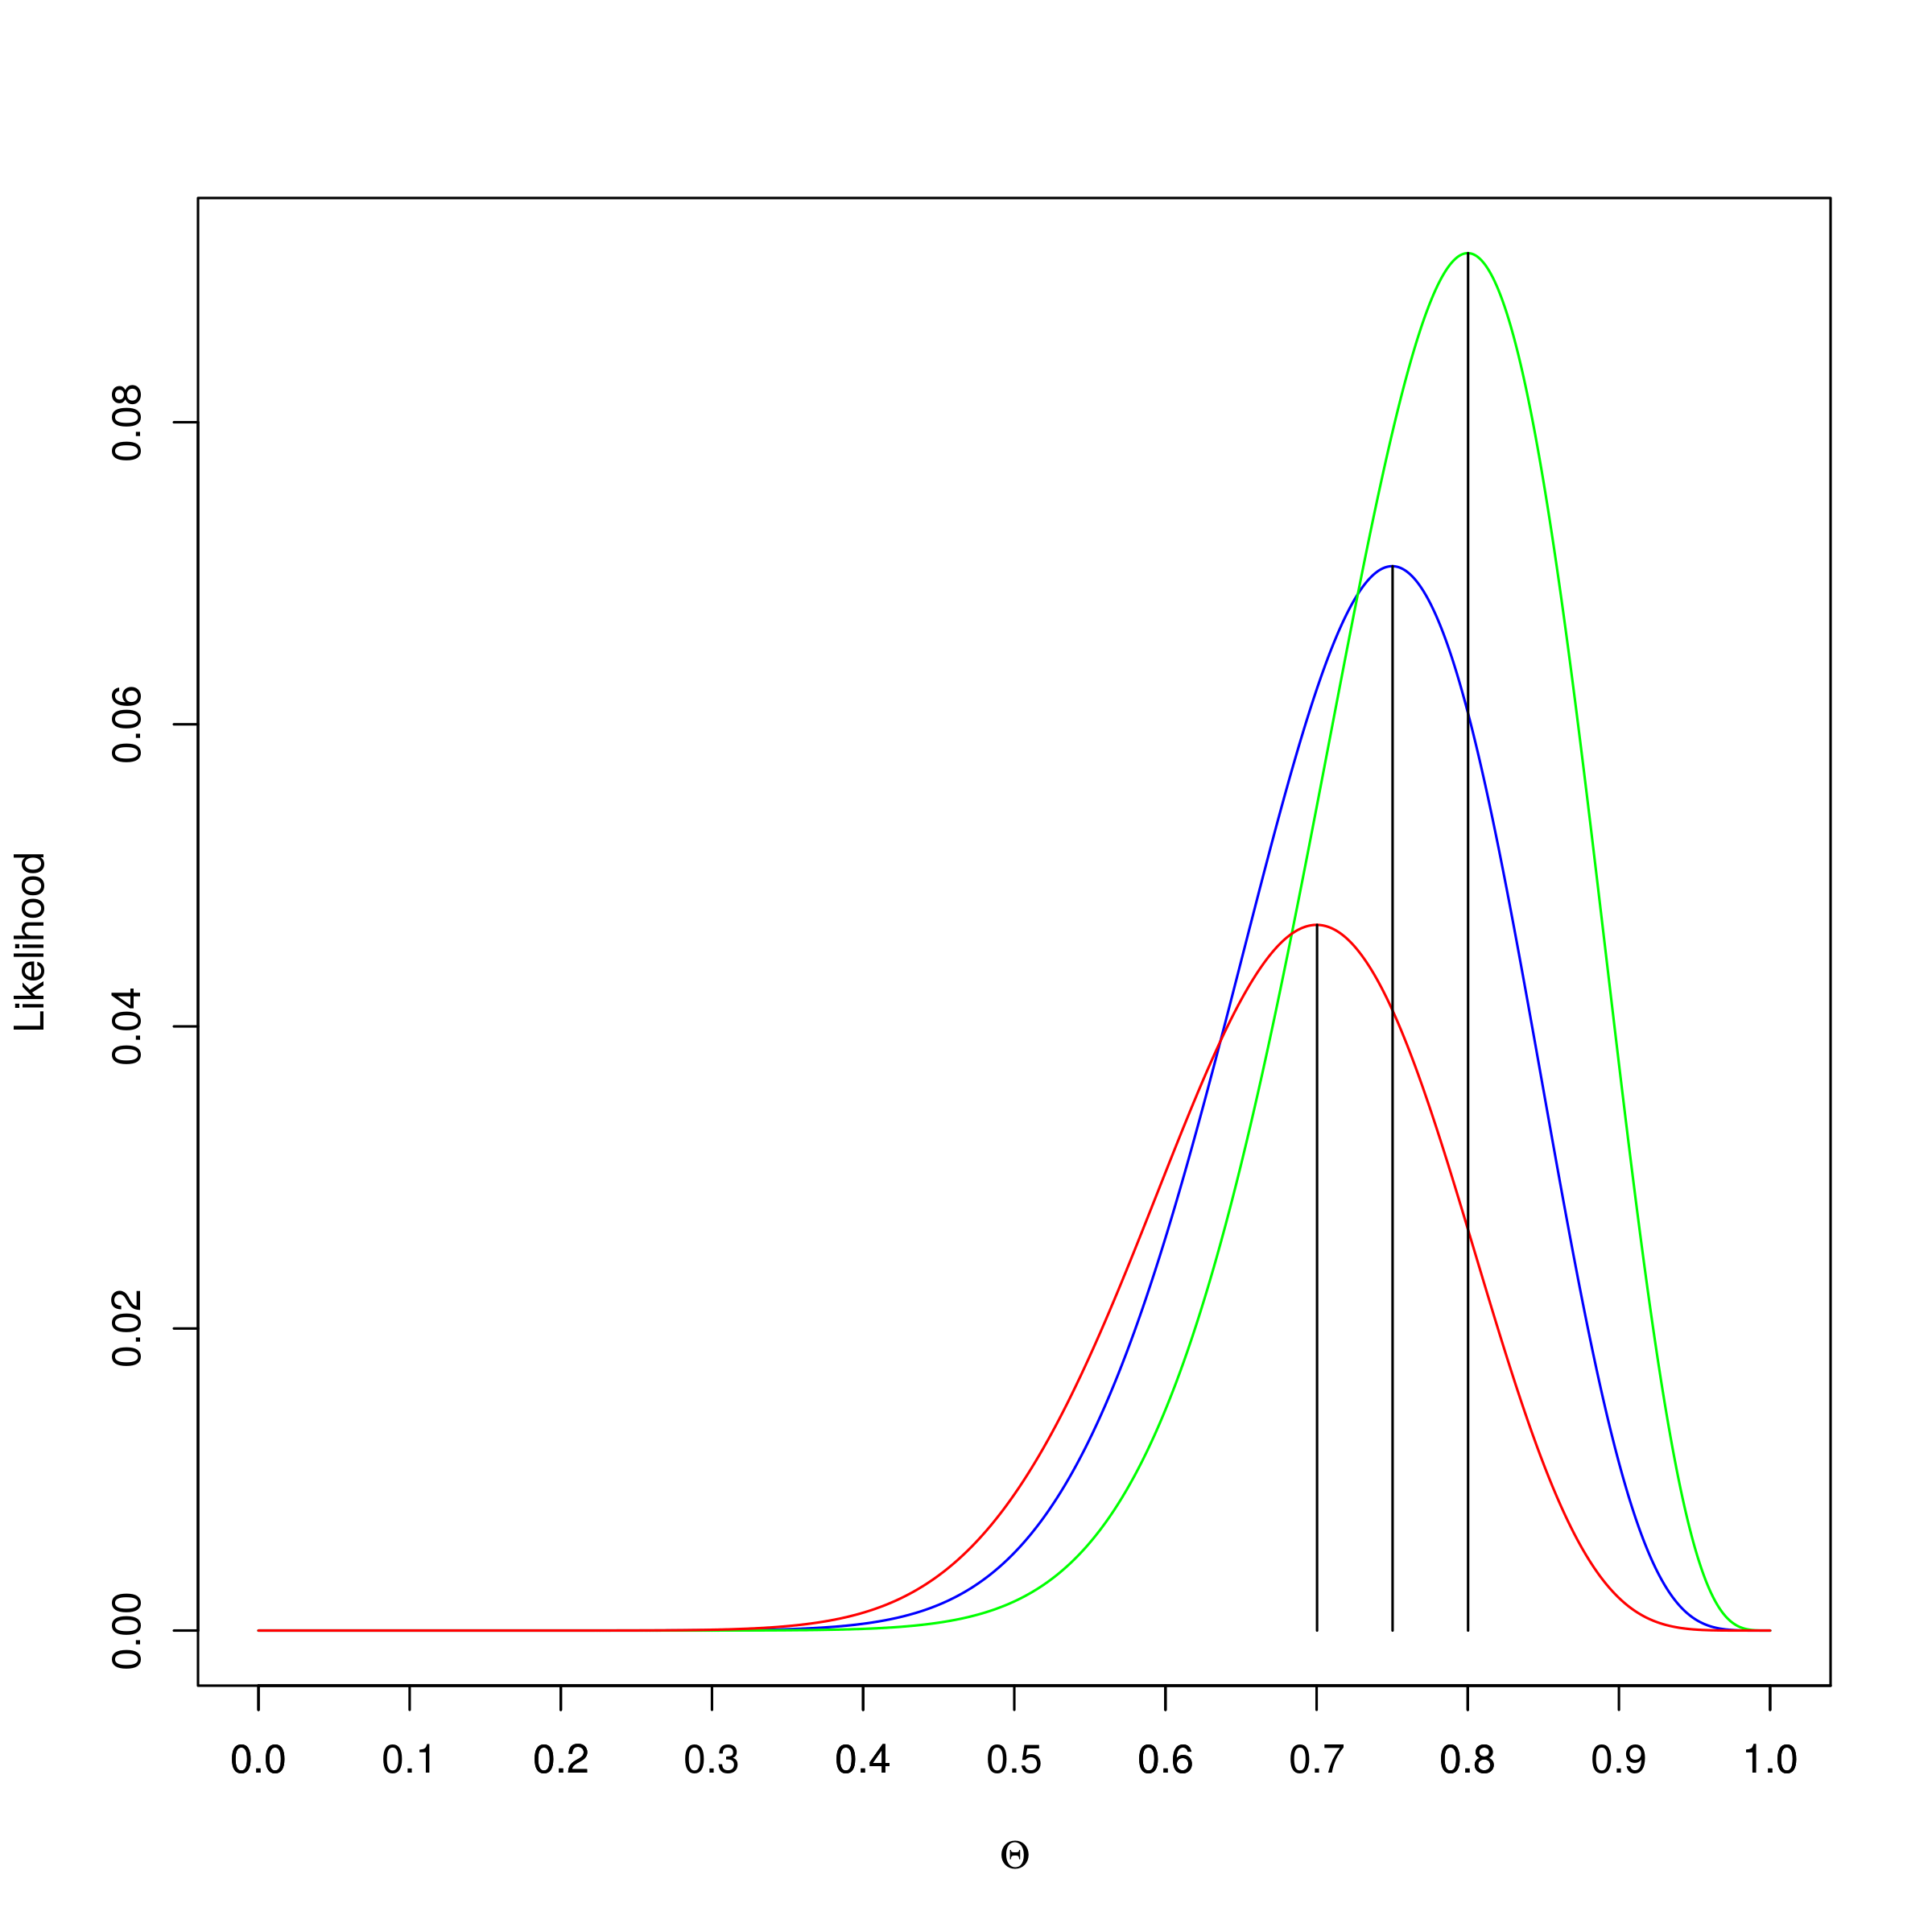
\includegraphics[scale=.3]{sparse_likelihood.png}
\caption{}
\label{fig:sparse_likelihood}
\end{subfigure}
~
\begin{subfigure}{.45\textwidth}
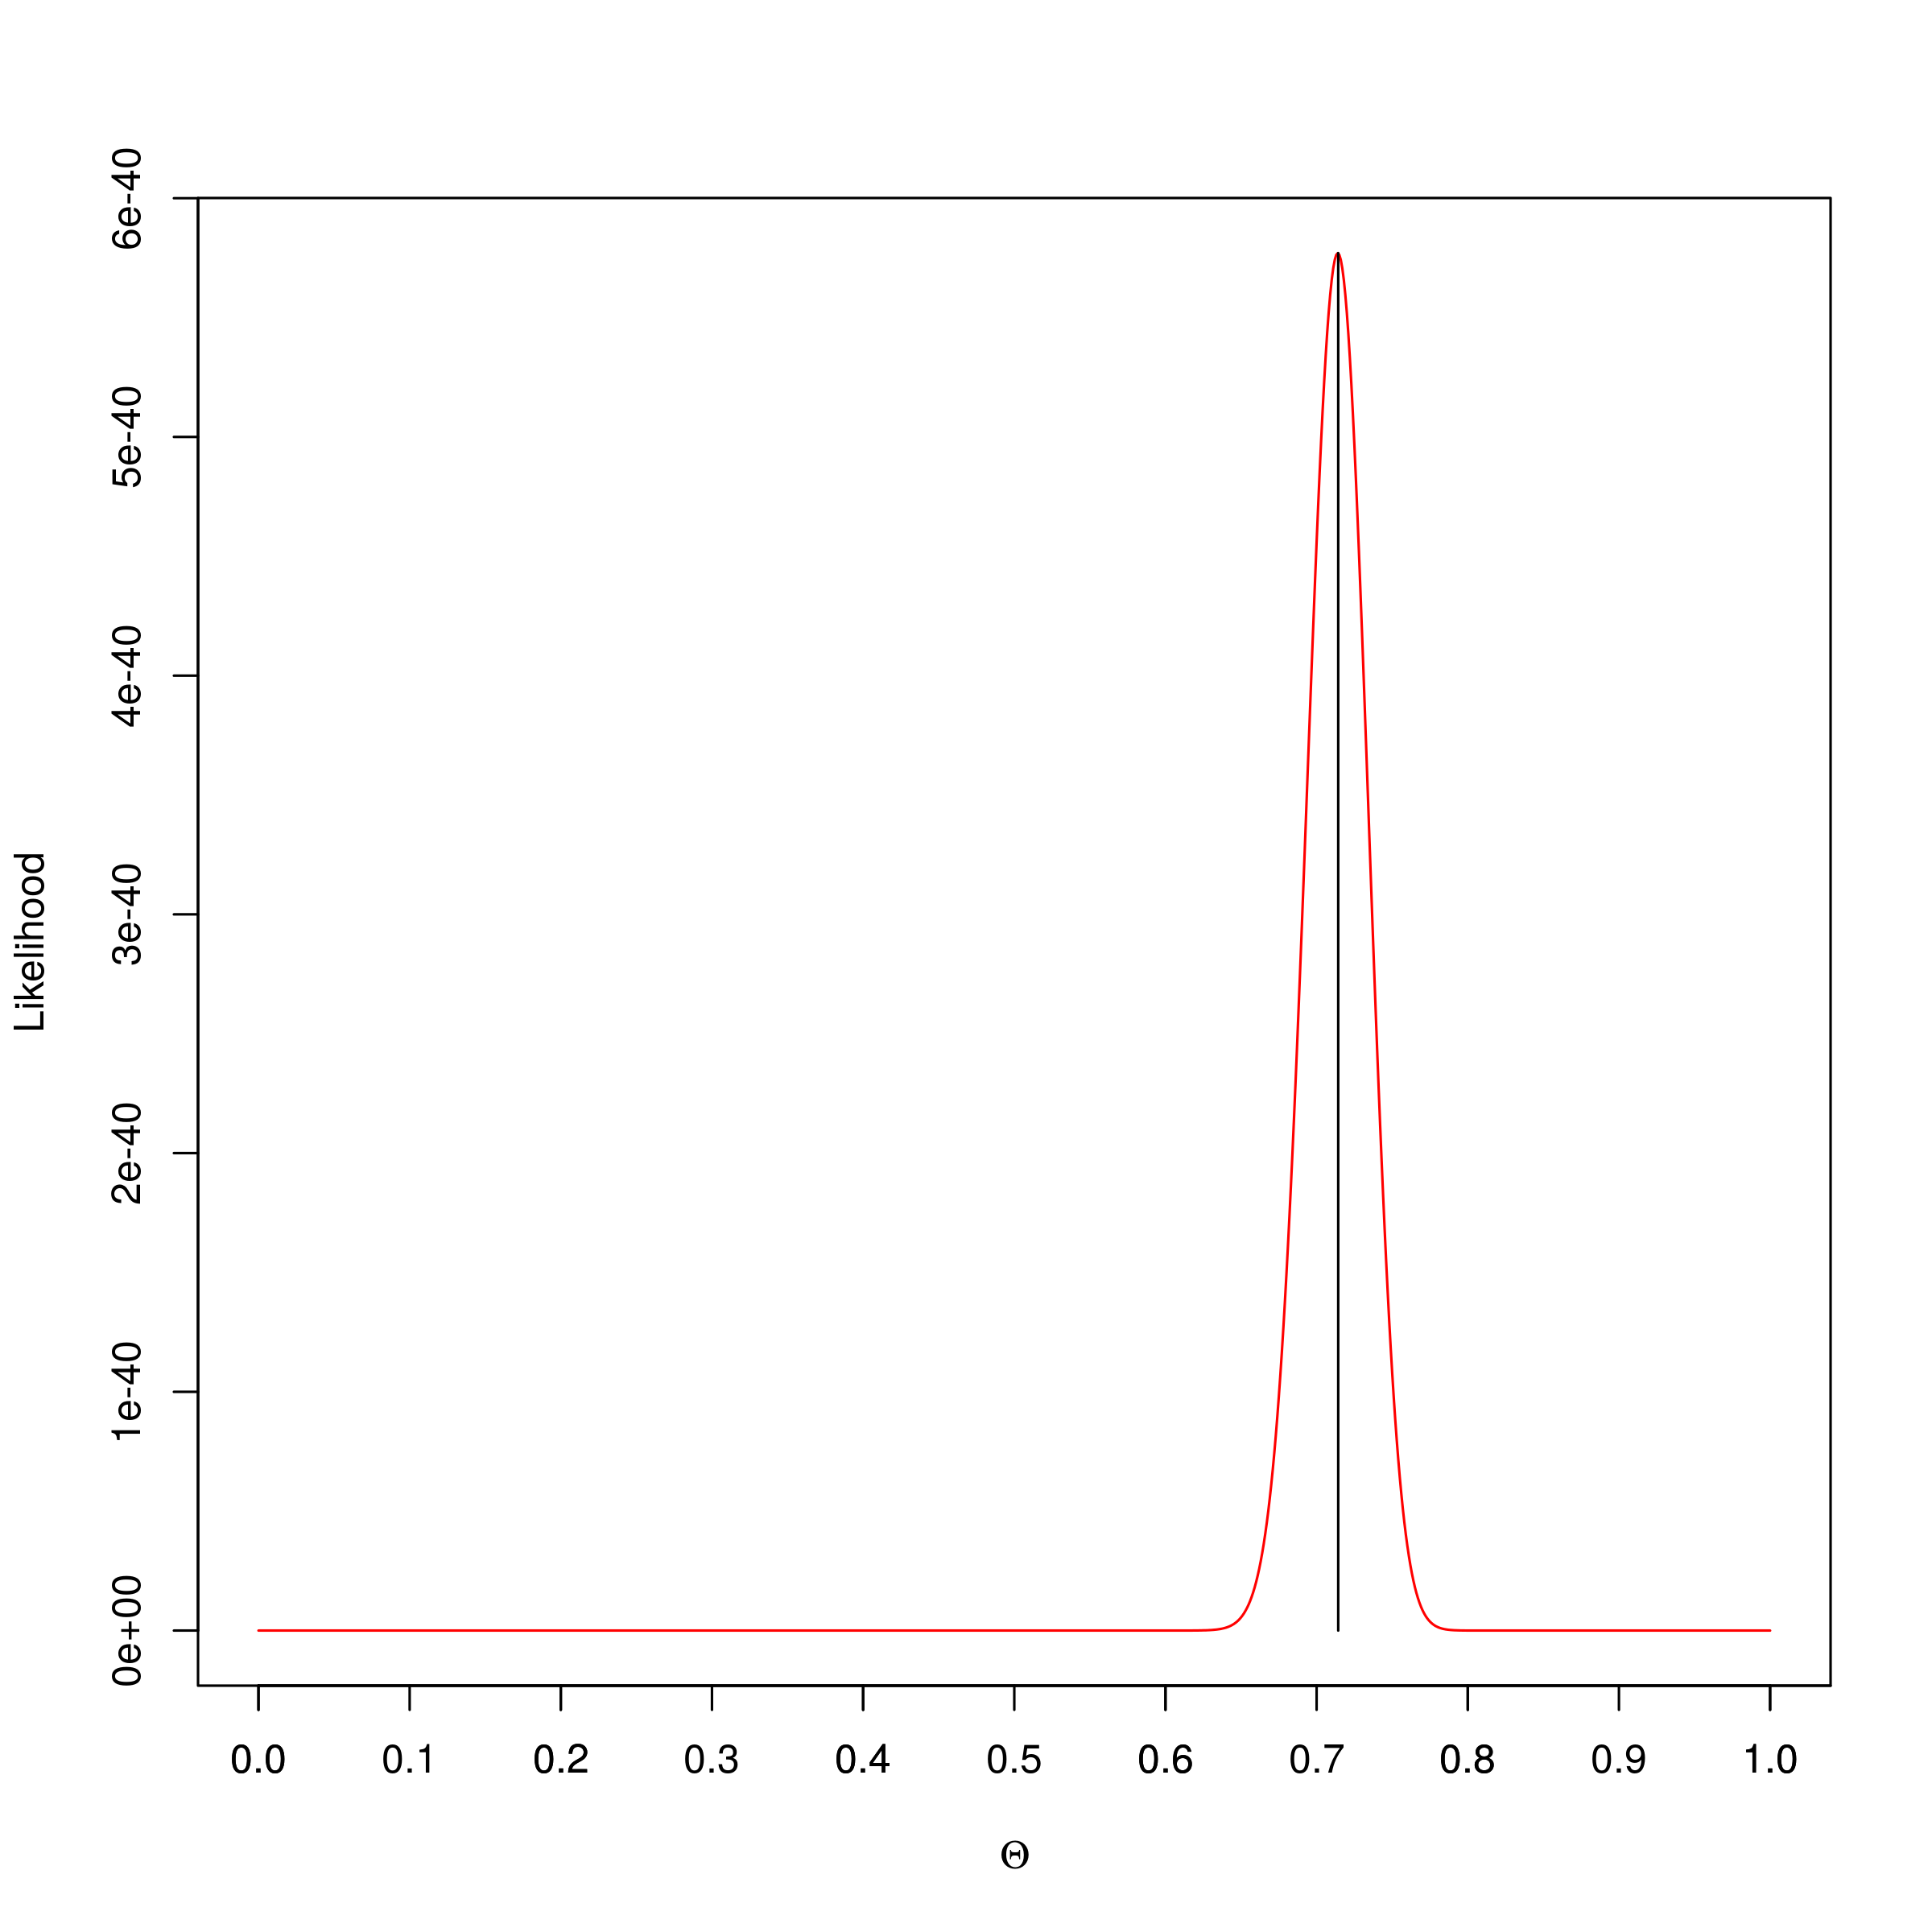
\includegraphics[scale=.3]{dense_likelihood.png}
\caption{}
\label{fig:dense_likelihood} 
\end{subfigure}
\caption{Plots of likelihood functions for different data samples. All data samples were randomly drawn
from a binomial distribution with parameters $ n=10 $ and $ \theta=0.7 $. Figure~\ref{fig:sparse_likelihood}
depicts the likelihood functions for data samples consisting of 2 draws each. The vertical lines indicate
at which value of $ \theta $ the likelihoods reach their maximums. Two draws contain relatively little
information about the underlying distribution and thus the likelihood function is fairly spread, indicating that there
are several parameter values that are about equally good.
Figure~\ref{fig:dense_likelihood}
shows the likelihood function for a data sample consisting of 50 draws. 50 draws convey much more information about the underlying distribution
and therefore the likelihood function is peaked around the MLE (which is also close to the true parameter $ 0.7 $. Deviating slightly from the MLE in his scenario
leads to a huge drop in likelihood, effectively ruling out a huge part of the parameter space as candidates for the true parameter.}
\label{fig:likelihood_plots}
\end{figure}

The maximum likelihood principle simply states that we should try to maximize the likelihood function of
our data, that is, we should pick the parameter value that achieves this maximisation. This parameter value
is known as the \textbf{maximum likelihood estimate} (or as maximum likelihood estimates if there are several). 

\begin{Definition}[Maximum Likelihood Estimate]
A maximum \\ likelihood estimate (MLE) for a parameter set~~$ \supp(\Theta) $ on a data sample $ x $ 
is a value $ \theta^{*} $ such that
$$ \theta^{*} = \underset{\theta}{\arg\max}\, \, L_{x}(\theta) $$
\end{Definition}

In Figure~\ref{fig:likelihood_plots} we have plotted some likelihood functions. They are based on data
samples that were randomly generated from a binomial distribution with parameters $ n=10 $ and 
$ \theta=0.7 $. The likelihood plots in Figure~\ref{fig:sparse_likelihood} are based on data sets of only
two samples, that is 20 i.i.d.\ Bernoulli trials. The plot in Figure~\ref{fig:dense_likelihood} is based on a 
data set of 50 samples, that is 500 i.i.d. Bernoulli trials. 
The vertical lines connect the maximum likelihood estimate
for each data set with its likelihood value. Notice the different scales of the two plots. The likelihood value depends on the
data size. Therefore, it does not make sense to compare likelihood values across data sets. After all, each data set comes with its own
likelihood function and the likelihood functions of different data sets are indeed different functions. This difference is also the
reason why the maximum likelihood principle tells us to only find the parameter value $ \theta $ at which the maximum of the
likelihood function is achieved. There is no point in even looking at the numerical likelihood value of that maximum.

Notice further that in Figure~\ref{fig:likelihood_plots}, there is only one MLE for each of these functions. We will shortly see why it is desirable for 
the likelihood function to only have one maximum.

Let us explain how to compute a MLE. By definition, the likelihood function maps the MLE to
one of its maximums. From calculus we know that the derivative of any differentiable function is 0 at the
function's maximums\footnote{Technically we also require that the function be defined on a closed 
(as opposed to open) interval. At this stage it is ok to assume that our parameter sets are always closed
intervals.}. Hence, all we need to do in order to find the MLE is to differentiate the likelihood 
function with respect to $ \theta $ and check where the derivative is 0. 
First, however, we need to write down the likelihood function.
Looking back at Definition~\ref{def:likelihood}, we recall that the likelihood is defined only
with respect to a probabilistic model. In order to write down a likelihood function, we need to first
define such a model. In other words, we have to define concrete likelihood functions on a case-by-case 
basis. We present one such case as an example below. Before we do so, let us note that for mathematical
convenience, one often uses the logarithm of the likelihood function instead of the likelihood function
itself. Taking the logarithm has two advantages: 1) logarithms turn products into sums and sums are often easier to handle
and 2) when using a computer, very small values may be rounded down to 0. Logarithms mitigate this problem
as they turn very small numbers into negative numbers that have rather large absolute values.

\begin{Definition}[Log-Likelihood]
For $n \in \mathbb{N} $ and a \emph{fixed} set of $n$ data points or observations $ x = x^{1}_{n} = x_1,x_2,\ldots,x_n $, we define the 
log-likelihood function over a 
family of distributions $ P_{x|\Theta} $ as 
$$ \mathcal{L}_{x}(\theta) := \log \left(L_{x}(\theta) \right) \ . $$
\end{Definition}

Notice that finding the maximum of the logarithm of any function $ f $ that only takes on positive values is the same as finding
the maximum of the original function $ f $. This is so because the logarithm function is strictly increasing, meaning that for any
two possible arguments $ x >y>0 $, we have $ \log(x) > \log(y) $ and hence, if $f(w) > f(z)$, we have $\log(f(w)) > \log(f(z))$.

In order to make it easier to find MLEs of your own, we give you a procedure that you can apply in most cases and
show you an example of how to use it.
\begin{enumerate}
\item Define a probabilistic model.
\item Write down the functional form of $ L_{x}(\theta) $ for the parameters of that model.
\item Write down $ \mathcal{L}_{x}(\theta) $.
\item Compute $ \frac{d}{d \theta} \mathcal{L}_{x}(\theta) $. This is also called the score function.
\item Solve $ 0 = \frac{d}{d \theta} \mathcal{L}_{x}(\theta) $ for $ \theta $.
\end{enumerate}

\paragraph{Example of finding the MLE} Assume we have to do market research for a clothing store in Amsterdam.
The store wants to expand its size and the manager wonders whether he should use the extra space to 
exhibit more men's or more women's clothing. To help him with this decision, we are going to count 
how many male and female customers are coming in on a given day. We treat the gender of each of the $n$ customers
as a random variable $ X_{i}$ and interpret $ X_{i} = 0 $ as male and $ X_{i} = 1 $ as
female. We assume that the underlying distribution that determines the gender of customers
is the same for all customers. We also assume that a customer's gender is independent of the gender of any
other customer. Hence, we stipulate that $ X_{i} \bot X_{j} $ whenever $ i \not = j $.

As an aside, notice that these assumptions are not without problems in real applications. 
The first assumption, that the gender
distribution is the same for all customers, may not always be justifiable. Depending on the time of the day,
it is possible that more men or women will come in. The second assumption, that the gender of one customer
does not depend on the gender of other customers, may also not always be true. If couples come to shop
at the store, then the gender of one partner will determine the gender of the other partner (in which
way the partners in a couple determine each other's genders depends on whether the couple is homo- or
heterosexual). For the sake of the example we will nevertheless assume that our assumptions hold true.

\textbf{Step 1:} As the day is over, we have observed $ k $ women and $ n-k $ men. Above, we postulated a model
according to which the
occurrences are distributed according a binomial distribution whose parameter $ n $ we already know: it
is simply the total number of our observations (a.k.a. the total number of customers who entered the shop 
that day). What we want in order to facilitate the manager's decision is to estimate $ \theta $, the
probability that a random customer is female. 

\textbf{Step 2:} Our likelihood function looks as follows:
\begin{equation}
L_{x}(\theta) = \binom{n}{k} \theta^{k} \times (1 - \theta)^{n-k} \ .
\end{equation}
As a mnemonic that $ \theta $ is unknown we can informally write
$$ L_{x}(\theta) = \binom{n}{k} ?^{k} \times (1-?)^{n-k} \ . $$

\textbf{Step 3:} We can now take the logarithm of our likelihood function.
\begin{align}
\log(L_{x}(\theta)) &= \log\left(\binom{n}{k} \theta^{k} \times \theta^{n-k} \right) \\
&= \log \left(\binom{n}{k}\right) + k\log(\theta) + (n-k)\log(1-\theta)
\end{align}

\textbf{Step 4:} To find the MLE, we first differentiate the log-likelihood with respect to $ \theta $.
\begin{align}
\frac{d}{d \theta} \mathcal{L}_{x}(\theta)
&= \frac{d}{d \theta} \log \left(\binom{n}{k}\right) + k \frac{d}{d \theta} \log(\theta) + (n-k) \frac{d}{d \theta} \log(1-\theta) \\
&= \dfrac{k}{\theta} - \dfrac{n-k}{1-\theta}
\end{align}

\textbf{Step 5:} Finally, we want to find a point where this derivative vanishes in order to find the maximum of $ \mathcal{L}_{x} $.
\begin{align}
0 &= \dfrac{k}{\theta} - \dfrac{n-k}{1-\theta} &\Leftrightarrow \\
\dfrac{n-k}{1- \theta} &= \dfrac{k}{\theta} &\Leftrightarrow \\
(n-k) \theta &= k (1 - \theta) &\Leftrightarrow \\
n\theta- k\theta &= k - k \theta &\Leftrightarrow \\
n\theta&= k &\Leftrightarrow \\
\theta &= \dfrac{k}{n}
\end{align}

And we are done! You know once and for all that the MLE for the parameter $\theta$ of \emph{any} binomial distribution with parameter $n$ (and having observed $k$ occurrences) is $ \frac{k}{n} $.

\begin{Exercise}
A coin is getting flipped 1000 times and comes up heads 600 times. According to the MLE, would you say that this coin is fair?
\end{Exercise}

Those who are already familiar with calculus may have felt a bit uncomfortable, because we simply state that setting the derivative of the log-likelihood
to 0 will give us a maximum of that function. In general, this technique will only give us an extremum which might as well be a minimum. How can we be so sure that
we really got a maximum? We will just do a proof by picture here and let you do the math. 

Take another look at Figure~\ref{fig:likelihood_plots}. Clearly, we only
see one maximum per function and that one is unique in all cases. 
What you cannot see in the plots is that the likelihood is never 0 for any $ \theta \in (0,1) $. It is just
really, really small, that is why it looks as if it was 0 in many places in the plot. What actually happens is that the likelihood is constantly decreasing as
$ \theta $ approaches 0 and 1. This constant decrease implies that the derivative is not equal to $ 0 $ anywhere other than at the maximum.

Finally, notice that the likelihood is only equal to 0 when $ \theta = 0 $ or $ \theta = 1 $. 
Thus, the likelihood function does indeed have two minima. However, these 
occur at the boundary points of the interval $ [0,1] $ and since we just stated that $ L_{x}(\theta) $ is constantly decreasing as $ \theta $ approaches those points,
we can safely conclude that the maximum does not lie on the boundary points. Hence, the only point at which the
derivative of the likelihood function of the binomial distribution is $ 0 $ is at the sole maximum.

We have mentioned above that having only one maximum is a desirable property. If we want to find the MLE, we have but one choice in this case. If there were
several maxima, we would have to compute all of them and pick amongst them. If there are two maxima that have equal likelihood values, we have no way of choosing
between them and thus no way of determining the single best parameter estimate. Moreover, we will encounter situations in the next chapter where it is very hard (if not
impossible) to find the global MLE (i.e.\ the MLE at the highest maximum).

You may rightfully wonder what distributions have the desirable property of only having one maximum in their likelihood functions. It turns out that those are
exactly the distributions in the \href{https://en.wikipedia.org/wiki/Exponential_family}{exponential family}. The link includes a list of those distributions and
you will be happy to see that most commonly used distributions are members of the exponential family and thus their likelihoods only have one maximum. Another feature of exponential family distributions is that
they all have sufficient statistics. Hence, whenever we are doing maximum likelihood estimation for 
an exponential family distribution, all we need to know about the data are the sufficient statistics. This
point will become important in the following chapter.

\begin{Exercise}
You are given some likelihood function $ L_{x} $ for the binomial distribution along with its MLE $ \theta^{*} $. Show rigorously that $ \theta^{*} $ is indeed
a maximum. That is, show that $ \mathcal{L}_{x}''(\theta^{*}) < 0 $, where $ \mathcal{L}_{x}'' $ is the second derivative of the log-likelihood function.
\end{Exercise}

 
\section{Maximum a Posteriori Estimation}

Recall that in Section~\ref{parameterEstimation} we set ourselves the goal of finding a good parameter estimate from the posterior distribution over parameters.
Let us say that the best parameter estimate is the one with the highest posterior probability. Then the question is: do we actually accomplish our goal with the MLE?
Does the MLE give us the parameter with the highest posterior probability? Unfortunately, the general answer is no, which becomes evident from Bayes' rule.
\begin{equation}
\underset{\theta}{\arg\max}~P(\Theta = \theta| X=x) = \underset{\theta}{\arg\max}~P(X=x|\Theta=\theta) \times P(\Theta = \theta)
\end{equation}

The MLE only maximises over the likelihood term but not over the prior! Hence it will in general be different from the \textbf{maximum a posteriori} estimate.

\begin{Definition}[Maximum a posteriori estimate]
A maximum a posteriori (MAP) estimate for a parameter set~~$\supp(\Theta)$ on a data sample $ x $ 
is a value $ \theta^{*} $ such that
$$ \theta^{*} = \underset{\theta}{\arg\max}\, \, P(\Theta = \theta| X=x) \ . $$
\end{Definition}

The MAP estimate can be derived with exactly the same steps as the MLE. However, parameters are usually real values which means that distributions over them
are continuous distributions. Since we have not dealt with continuous distributions in this course, we will stop just short of actually imposing
(non-uniform) prior distributions over parameters and computing MAP estimates.

Notice that up to now, we justified the maximum likelihood principle merely from intuition by postulating that high likelihood should somehow be an indicator for
good parameter values. We will now justify the maximum likelihood principle more formally, by showing that the MLE is just a special kind of MAP estimate. Since
this realisation implies that under certain condition the MLE will also have the highest posterior probability, we can safely argue for the MLE based on its posterior probability.

Let us assume that our prior distribution $ P_{\Theta} $ over parameters is uniform. Then we can write the MAP estimator\footnote{If you know some continuous probability
theory: the MAP estimate is taken on the posterior density function in this case since the distribution over parameters is continuous.} as
\begin{align}
&\underset{\theta}{\arg\max}\, \, \frac{\partial}{\partial\theta} \log (P(\Theta = \theta| X=x)) \\
= &\underset{\theta}{\arg\max}\, \, \frac{\partial}{\partial\theta}\log (P(X=x|\Theta=\theta) \times P(\Theta = \theta)) \\
= &\underset{\theta}{\arg\max}\, \, \frac{\partial}{\partial\theta}\log (P(X=x|\Theta=\theta)) + \log(P(\Theta = \theta)) \label{eq:posteriorDiff} \\
= &\underset{\theta}{\arg\max}\, \, \frac{\partial}{\partial\theta}\log (P(X=x|\Theta=\theta)) \label{eq:MLE=MAP} \, ,
\end{align}
where we used the uniformity of $\Theta$ to get from \eqref{eq:posteriorDiff} to \eqref{eq:MLE=MAP}. We can neglect $ \log(P(\Theta = \theta) $ when finding the maximum, because if we add a constant to all likelihood values, the MLE will not change.

This derivation tells us that if we choose a uniform parameter prior, the MLE will be the MAP estimate. Hence, what we are actually assuming whenever we choose the MLE as
our parameter estimate, is that our prior over parameters is uniform. This is a very strong assumption to make and one may rightfully criticise the maximum likelihood principle because of this assumption (actually one should).

Let us conclude this section by saying that for the rest of this course we will make the assumption that we are using uniform parameter priors with justification.
This means that we can safely use the MLE in order to find the parameter value with the highest posterior probability.


\section*{Further reading}
If your calculus is a bit rusty or you have never taken a calculus class before, you should consult 
\href{https://www.coursera.org/learn/calculus1}{OSU's excellent (and very fun) online course} which allows you to learn at your own pace. The course also comes with
\href{https://mooculus.osu.edu/handouts}{a lecture script} that contains many insightful examples and exercises. Let us emphasise that doing statistics (including
machine learning) without a solid understanding of calculus is close to impossible.

If you are looking for a good introduction to
parameter estimation that covers everything we have discussed here and also goes a considerable stretch further, we refer you to 
\href{http://www.arbylon.net/publications/text-est.pdf}{Gregor Heinrich's widely cited tutorial}. Heinrich's examples come from text modelling but the techniques he
describes can be applied anywhere. One of the model he discusses, \href{https://en.wikipedia.org/wiki/Latent_Dirichlet_allocation}{Latent Dirichlet Allocation}, originates
from text modelling but has wide-spread applications in biology, as well.


%%% Local Variables:
%%% mode: latex
%%% TeX-master: "chapter5"
%%% End:




\chapter{The EM Algorithm}

\section{Mixture Models}\label{sec:mixtureModels}

In the previous chapter we have mentioned that it may happen that a likelihood function has multiple 
maxima and that sometimes it may be hard or impossible to find the global maximum (i.e.\ the maximum
with the overall highest likelihood value). Such a situation occurs whenever the probabilistic model
that we use to model our observations is a \textbf{latent-} or \textbf{hidden-variable model}. Latent-variable
models are models that besides modelling observed data also model a portion of unobserved data. For
example, if we look at the income distribution of a population we may want to further differentiate
between age groups. If the age of all or some members of the population is not provided in the data, we
can still model it as a latent variable. The difficulty is that we will have to make inferences about the
age of an individual based on other information that we have about it (e.g.\ the income). 

While it may in general be quite hard to formulate latent-variable models, there are certain standard
latent-variable models that have wide-spread applications. One such class are \textbf{mixture models}.

\begin{Definition}[Mixture Model]\label{def:mixtureModel}
We assume jointly distributed random variables $ X=X_{1}^{n} $ and $
Y=Y_{1}^{n} $ where $ Y $ is \href{https://en.wikipedia.org/wiki/Categorical_variable}{categorical} (as defined on Page~\pageref{lab:categorical}) and
$ supp(Y) = \{c_{1}, \ldots, c_{k}\} $. The $ X_{i} $ are observed data, the $ Y_{i} $ are latent
or observed and the $ c_{j}, 1\leq j \leq k $ are called mixture components. 
If the distribution
$ P(X_{1}^{n}=x_{1}^{n}, Y_{1}^{n} = y_{1}^{n}\mid \Theta = \theta) $ factors as
\begin{align*}
&P(X_{1}^{n}=x_{1}^{n}, Y_{1}^{n} = Y_{1}^{n}\mid \Theta = \theta)  \\
&= P(Y_{1}^{n} = y_{1}^{n}\mid \Theta = \theta) \prod_{i=1}^{n} 
P(X_{i}=x_{i} \mid Y_{i} = y_{i}\mid \Theta = \theta) \ .
\end{align*}
we call this model a \emph{mixture model}. The marginal probabilities $ P(Y_{i}=y_{i}) $ for $ 1 \leq i \leq n $ are called
\emph{mixture weights}.
\end{Definition}

Mixture models are extremely useful whenever we have different ways to think about our data. Each way
of conceptualising our data can be encoded by one of the mixture components of the mixture model. The modelling
of the data under that view is done by the conditional distribution induced by the mixture component.
This technique can help us to build a better overall model of our data. Let us introduce a running example that
we use for the rest of this section. A graphical depiction of the model used in the example is given in Figure~\ref{fig:mixtureGraphical}.

\paragraph{Notation} Notice that throughout this chapter we use $ \Theta $ as a generic variable over collections of parameters. Assume any
model that has parameters $ p $ and $ q $. Then we have $ \Theta = (p,q) $. For the time being you can thus regard the conditioning on $ \Theta = \theta $
as an underspecified dependence on any parameters that the model may have. We will become more concrete about parameter values in Section~\ref{sec:EMExample}.
\begin{figure}
\center
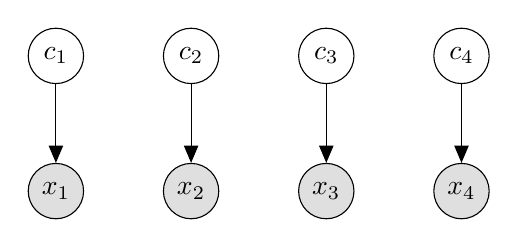
\begin{tikzpicture}
\node[latent] 					(c1)		{$ c_{1} $};
\node[latent, right = of c1] 	(c2) 	{$ c_{2} $};
\node[latent, right = of c2] 	(c3) 	{$ c_{3} $};
\node[latent, right = of c3] 	(c4) 	{$ c_{4} $};

\node[obs, below = of c1] (x1) {$ x_{1} $};
\node[obs, below = of c2] (x2) {$ x_{2} $};
\node[obs, below = of c3] (x3) {$ x_{3} $};
\node[obs, below = of c4] (x4) {$ x_{4} $};

\edge{c1}{x1};
\edge{c2}{x2};
\edge{c3}{x3};
\edge{c4}{x4};
\end{tikzpicture}
\caption{A graphical model of the mixture model used in our
  example. Only four data points are shown. Shaded nodes indicate observed values, light nodes indicate
latent values. A graphical model shows the dependencies between variables in a probabilistic model. In this example we see that a) the latent variables
are independent of each other and b) the observed variables are independent given the latent variables. (Aside: formally the graphical model actually shows the
\textit{independencies} assumed by our model! Reasoning about it in terms of dependencies is often easier, though.)}
\label{fig:mixtureGraphical}
\end{figure}

\paragraph{Example of a mixture model} Assume we observe 20 sequences of coin tosses. Each sequence
contains 10 flips. We also know that there are 3 coins with which these sequences could possibly have been
generated and for each sequence a different coin may have been used. We want to find out what the biases
of the coins are (i.e.\ the parameters of the binomial distributions associated with the coins) and the probability
for each coin to have generated a particular sequence.
 
We could assume that the entire data set was generated by exactly one coin. We would then employ maximum likelihood estimation 
to find the parameter of that coin. However, this model might actually turn out to be
pretty bad because we are committing to picking one coin only. This is
a bad assumption, because we know that each sequence may have been generated by a different coin. 

A mixture model comes to the rescue. Instead of assuming that only one coin has generated all 20 sequences,
we assume that all three coins have contributed to generating the 20 sequences. However, their contributions
may not be equal. This inequality is exactly what the mixture weights capture. 

In order to model the contribution of each coin, we introduce a latent RV $ Y $ over mixture components with labels $ c_{1}, c_{2}, c_{3} $ representing the three coins.
In the present case, each mixture component is linked to a binomial distribution, parametrized by the biases of
the coins. We will also adopt the often-used assumption
that the mixture components are independent of each other. This means that the coin that generated each
sequence of coin flips was chosen independently of the coins used for the other sequences. Our independence assumptions
are also encoded in the graphical model in Figure~\eqref{fig:mixtureGraphical}. As usual, we call our data $ x $. 
This information suffices to formulate our mixture model.
\begin{align} 
&P(X_1^n=x_{1}^{n},Y_{1}^{n}=y_{1}^{n}\mid \Theta=\theta) \label{eq:mixtureExample} \\
&= \prod_{i=1}^{n} P(Y_{i}= y_{i} \mid \Theta=\theta)P(X_{i}=x_{i} \mid Y_{i}=y_{i},\Theta=\theta) \nonumber 
\end{align}

Notice that if we were given the mixture weights, estimating
the parameters of the mixture components would be easy: we would simply find the MLE for each mixture component separately. The mixture
model could then easily be constructed because the mixture weights are known. 

Usually, we face a more difficult problem when working with mixture models. Neither the mixture
weights nor the parameters of the mixture components are known. In this case, doing straighforward MLE is impossible because the data is
incomplete\footnote{Incomplete data is 
  another name for a collection of random variables of which some have unobservable (latent) outcomes. Data modelled with a mixture model is incomplete because it contains
  an observed part (the number of heads in our example) and a latent
  part (the mixture components which in our example are the types of coin). In general, whenever you have complete data, analytic MLE computation is possible. The moment your data is incomplete, it becomes impossible.}. 

How can we go about estimating the model parameters, i.e.\ the parameters of the mixture components and the mixture weights?
Each factor
in \eqref{eq:mixtureExample} is in fact a joint distribution (by the chain rule). We exploit this to rewrite the model as a model of the
observed data only.
%\begin{align}\label{eq:marginal}
%P(X_1^n=x_{1}^{n} \mid  \Theta= \theta) &= \prod_{i=1}^{n} \sum_{j=1}^{3} P(X_{i}=x_{i},Y_{i}=c_{j} \mid  \Theta= \theta)
%\end{align}
%\philip{Compare this to Equation~\eqref{eq:mixtureExample}. There we constructed a probability distribution over the joint outcomes $ X_{1}^{n} $ and
%$ Y_{1}^{n} $. Because we assumed independence between mixture components, the distribution could be factorised over pairs $ (X_{i},Y_{i})$ for $ 1 \leq i \leq n $.
%In Equation~\eqref{eq:marginal} we then inferred the marginal distribution for $ X_{1}^{n} $. Recall that in order to compute the marginal of $ X_{1}^{n} $ we
%need to sum over all possible $ Y_{1}^{n} $. Because their joint distribution factorises nicely, we can perform the marginalisation per $ (X_{i},Y_{i})$ pair.
%This is exactly what is happening in Equation~\eqref{eq:marginal}. 
%Please pay attention to a crucial notational difference between \eqref{eq:mixtureExample} and
%\eqref{eq:marginal}: In the former we wrote $ Y_{i}=y_{i} $ whilst in the latter we wrote $ Y_{i}=c_{j} $. Why did we do this? Equation~\eqref{eq:mixtureExample} is
%a joint distribution and thus $ Y_{i} $ needs to take on a \textit{specific} value $ y_{i} \in \{c_{1},c_{2},c_{3}\} $. To get the marginal distribution of
%$ X_{i} $, however, we need to sum over \textit{all} values that $ Y_{i} $ can take on. We do this by writing $ Y_{i} = c_{j} $ which provides us with a means
%of summing over the possible outcomes $ c_{1},c_{2},c_{3} $.}
%\chris{this is going too fast! I don't understand it, you also
%  switched from $y_1^n$ to $c_j$ somehow... where did you use
%  \eqref{eq:mixtureExample} here??}\philip{Sorry, the conditioning was wrong in 6.1. Please check whether the above explanation helps you to understand what's going
%  on now.}
% \begin{align}\label{eq:marginal}
% P(X=x_{1}^{n} \mid  \Theta= \theta) &= \sum_{j=1}^3 P(Y_i = c_j)
%                                  P(X=x_{1}^{n} \mid Y_{1}^{n}=y_{1}^{n},\Theta=\theta)
%   \\
% &=  \prod_{i=1}^{n} \sum_{j=1}^{3} P(X_{i}=x_{1},Y_{i}=c_{j} \mid  \Theta= \theta)
% \end{align}

\begin{align}
P(X_1^n=x_{1}^{n} \mid \Theta= \theta) &= \sum_{j_1=1}^3 \sum_{j_2=1}^3 \cdots \sum_{j_n=1}^3 P(X_1^n=x_{1}^{n}, Y_1=c_{j_1}, \ldots, Y_n=c_{j_n} \mid \Theta= \theta) \label{eq:marginal} \\
&= \sum_{j_1=1}^3 \sum_{j_2=1}^3 \cdots \sum_{j_n=1}^3 \prod_{i=1}^{n} P(X_{i}=x_{i},Y_{i}=c_{j_i} \mid  \Theta= \theta) \nonumber \\
&= \prod_{i=1}^{n} \sum_{j=1}^3 P(X_{i}=x_{i},Y_{i}=c_{j} \mid  \Theta= \theta) \, , \nonumber
\end{align}
where the second equality uses the fact that we have assumed independence between the mixture components and hence
the expression $P(X_1^n=x_1^n, Y_1^n=y_1^n \mid \Theta = \theta)$ factorizes.
Now that we have related mixture models to the probability of the observed data, we can hope to estimate
their parameters using the maximum-likelihood principle.

There is one remaining problem, however: if the mixture weights $P(Y_i=y_i)$ are unknown, there is no closed-form solution for estimating the likelihood function. This is because
the likelihood depends on the parameters of the mixture components whose distribution, given
by the mixture weights, is unknown. This means that while we can compute the likelihood for each
individual mixture component, we cannot compute the likelihood of the entire mixture model because we
do not know how much each component contributes to the overall likelihood term. As a consequence, we can not 
simply apply calculus as we have been doing up to now. For this reason, we turn to the \textbf{EM algorithm}, 
that allows to at least find a local maximum of the likelihood function.

One final note: At the beginning we introduced latent-variable models (and hence mixture models) as models
of \textit{latent data}. We have cast the problem of inferring the mixture weights as inferring a 
distribution over mixture components, however. One may argue that those are not data, neither latent nor 
observed. This is a fair criticism but there is an easy way out. Simply imagine that each sequence of coin
flips was annotated with a pointer to the mixture component (the coin) that generated it. This annotation
is clearly part of the data. Since in our actual data, these annotations are missing, we treat them as 
latent data.

\section{The EM Algorithm}

In order to estimate the parameters of mixture models, we can employ a classical algorithm of 
\textbf{unsupervised learning}\footnote{Whenever the feature of our
  data that we want to predict (such as the coin which generated a sequence)
is observed, we speak of supervised learning. If the target feature is latent, we speak of unsupervised learning.}, 
namely the \textbf{expectation-maximisation (EM) algorithm}. This
algorithm allows to find a local maximum of the likelihood function of mixture models or, more
generally, models with missing data. 

\paragraph{Another example of latent data.} To give you some more intuition for what latent data is we provide a further example that has
spawned a lot of research. Assume you run a website that recommends movies
based on a user's preferences. In order to make statistical predictions about what type of user
likes what kind of movie, you ask your users to rate movies according to different categories.
Say you ask your users to rate the movies for entertainment value, action and fun. What may happen is
that some of your users only rate a movie in one or two of these three categories. However, these
ratings are still valuable to you and you do not want to throw them away, just because the rating is
incomplete. Thus you have a data set with some missing data that you have to fill in somehow.
\bigskip

In mixture models, annotations that tell you which mixture component
generated a given data point can be thought of as missing data. As we have seen, such annotations
are usually missing and thus we cannot do maximum likelihood estimation. The idea of EM is to
make an educated guess at the probability with which each mixture component could \textit{potentially}
have generated a data point $ x_{i} $. What we do know is our observed data and some initial guess of the mixture
weights which act as prior probabilities for the mixture components (this guess may be arbitrary). 
Our educated guess is then simply based on Bayes' rule. It is the posterior probability of each mixture
component given the data point $ x_{i} $.

Using the posterior over the latent (missing) data, the EM algorithm allows us to probabilistically fill in the missing data and find good mixture weights
(where you should understand \textit{good} in the maximum-likelihood sense). The idea behind the
algorithm is simple: first, compute the expected number of occurrences of the missing data values (the mixture 
components). Then treat these expectations as observed and do maximum likelihood estimation as usual\footnote{Notice that expectations can take on non-integer values and thus when treating them as observations we are handling a dataset with ``fractional'' observations. While this may be conceptually awkward
it does not change the mathematics of maximum likelihood estimation.}. Repeat the procedure 
until the likelihood does not increase any further. Notice that this procedure requires to
fix the number of mixture components in advance.

More formally, assume a data set $ X=x $. Furthermore, define $ Y $ as a random variable over latent data that can
take on $ |\mathcal{Y}| $ possible values $c_1, c_2, \ldots, c_{|\mathcal{Y}|}$. Then the likelihood function is 
\begin{align}
L_{x}(\theta) = P(X=x \mid \Theta=\theta) = \underset{j=1}{\overset{|\mathcal{Y}|}{\sum}} P(X=x, Y=c_{j} \mid \Theta=\theta)
\end{align}
where $ \Theta $ ranges over the parameters of the joint distributiforon $ P_{XY} $. Recall that EM
probabilistically fills in missing data. However, since we are doing maximum likelihood estimation, we
are not so much interested in the missing data itself but rather in the sufficient statistics of
that data (see Section~\ref{sec:sufficientStats}). Since we cannot directly obtain the sufficient statistics
of missing data, we will instead compute the \textit{expected sufficient statistics}\footnote{
Because we are referring to sufficient statistics our exposition of EM is specific to distributions
in the exponential family. The EM algorithm can also be made more general. However, since virtually
all distributions of interest in practice do belong to the exponential family, we will not make this kind of generalisation.
}.

The EM algorithm is an iterative 
algorithm, meaning we repeat its steps several
times. We use superscripts to indicate the number $l$ of the repetition, where $ 0 \leq l \leq k $.
To formalize the EM algorithm, assume we are at iteration $l$ for which we have some parameter estimate 
$\theta^{(l)} $ (the initial estimate $\theta^{(0)}$ can be set arbitrarily). Based on this parameter 
estimate we then compute the expected sufficient statistics of our model which we will call $ t(y,x) $.
\begin{equation} \label{Estep}
t(y,x)^{(l+1)} = \E(t(Y,x) \mid X = x,\Theta = \theta^{(l)})
\end{equation} 
%\chris{would it make sense to always write $\E_Y(\ldots)$ to indicate where the expectation is taken over?}\philip{Yeah, I guess we could do that. Do you think we'd have
%to explain that kind of notation or would people understand it?}

Equation~\eqref{Estep} is known as the \textbf{E(xpectation)-step} of the EM algorithm. This name
comes from the fact that in this step we compute the expected sufficient statistics. 
To make the algorithm complete, we still miss a
\textbf{M(aximization)-step}. But that step is simple. We pretend that the expected sufficient statistics of 
the latent data were actually observed. Once we pretend to observe the expected statistics, the maximization 
step can be performed using the maximum-likelihood estimation:
\begin{equation} \label{Mstep}
\theta^{(l+1)} = \underset{\theta}{\arg\max} \, P(X=x, t(Y,X) = t(y,x)^{(l+1)} \mid \theta)
\end{equation}

\begin{Definition}[EM algorithm]\label{def:EM}
We assume a data set $ x $ and postulate that there is unobserved data $ y $. We also
assume a probabilistic model $ P(X=x,Y=y \mid \Theta = \theta) $ whose parameters are realisations of a RV
$ \Theta $. Let $ t(x,y) $ be the sufficient statistics for that model. Then any
iterative algorithm with $ m $ iterations that performs the following
steps for $0\leq l \leq m-1$, 
\begin{align*}
\mbox{\textbf{E-step:} } \quad t(y,x)^{(l+1)} &= \E(t(Y,x) \mid X = x, \Theta = \theta^{(l)}) \\
\mbox{\textbf{M-step:} } \qquad \theta^{(l+1)} &= \underset{\theta}{\arg\max} \; P(X=x, t(Y,X) = t(y,x)^{(l+1)} \mid \Theta = \theta) 
\end{align*}
to update the model parameters is called an EM algorithm. 
\end{Definition}

\section{Example of an EM Algorithm for a Mixture Model}\label{sec:EMExample}

Assume as in Section~\ref{sec:mixtureModels} that our data is $ x=x^{20}_{1} $ where each $ x_{i} $ is the 
number of heads that we observed in a sequence of a 10 coin tosses. Again we also assume mixture components representing three coins which are linked
to binomials with parameters representing the biases of the coins. 
The latent data in this case is an annotation that for each observed sequence $ x_{i} $ reveals the coin that has been used
to generate that sequence. Thus we have latent data $ y=y_{1}^{n} $ where each $ y_{i} $ can be one of the three mixture components. 
We make the additional assumption that choosing a coin to generate a particular sequence is done independently of the coins chosen
to generate all the other sequences. This has the effect that in our model the latent data points will be independent\footnote{The assumption
that the mixture components in a mixture model are independent is actually quite common.}.

In this example, our collection of parameters $ \theta $ consists of two group of parameters, namely $ w_{1}, w_{2}, w_{3} $ for the mixture
weights and $ \phi_{1}, \phi_{2}, \phi_{3} $ which are the parameters of the binomials linked to the mixture components (i.e. these parameters
represent the biases of the coins). When we condition on $ \theta $, we will often not need all of the parameters in the collection. For example,
\begin{align*}
P(Y=c_{1}|\Theta=\theta) = P(Y=c_{1}|W_{1}=w_{1}) = w_{1}
\end{align*}
because the first mixture weight is the only parameter that is needed to compute 
the probability of observing the mixture component $ c_{1} $. 

Notice that because the mixture components are categorically distributed we have the constraint that
$ w_{1} + w_{2} + w_{3} = 1 $. Furthermore because $ \phi_{1}, \phi_{2}, \phi_{3} $ are binomial parameters, we know that they have to lie in $ [0,1] $.

\paragraph{E-step} Initially we arbitrarily assume that the coins have biases of $ 0.4, 0.5  $ and $ 0.65 $, meaning that we initialize the binomial parameters of the data-generating
distributions as follows:
\begin{equation}
\phi^{(0)}_{1} = 0.4 \hskip 0.5cm  \phi^{(0)}_{2} = 0.5 \hskip 0.5cm  \phi^{(0)}_{3} = 0.65
\end{equation}
We also assume that the fair coin is more likely to be used and hence set its initial mixture weight to $ w_2^{(0)}=0.5 $ and the mixture weights of the 
other two coins to $ w_1^{(0)}=w_3^{(0)}=0.25 $ (any other choice would also be fine). Let 
us take a closer look at our data. To shorten notation, we write it as a list where the i$ ^{th} $ entry is the value of $ x_{i} $.
$$ \left[ 6, 5, 4, 2, 2, 6, 5, 5, 4, 2, 5, 2, 4, 4, 6, 4, 5, 6, 3, 3 \right] $$ 
Then for each $ x_{i} $ we check how likely each coin is to have generated that point. In order to compute the posterior for each coin given a data point, we need
the likelihood for that data point. For the first observation we get the following likelihood values.


\begin{align}
&P(X_{1}=6 \mid Y_{1} = c_{1}, \Theta=\theta^{(0)}) = P(X_{1}=6 \mid Y_{1}=c_{1},\Phi_{1} = 0.4) = 0.1114767& \\
&P(X_{1}=6 \mid Y_{1} = c_{2}, \Theta=\theta^{(0)}) = P(X_{1}=6 \mid Y_{1}=c_{2},\Phi_{2} = 0.5) = 0.2050781& \nonumber \\ 
&P(X_{1}=6 \mid Y_{1} = c_{3}, \Theta=\theta^{(0)}) = P(X_{1}=6 \mid Y_{1}=c_{3},\Phi_{3} = 0.65) = 0.2376685& \nonumber
\end{align}

Recall that the mixture weights are nothing else than priors over mixture components. Hence, in order to get the joint distribution over observed and
latent data, we multiply the likelihoods by the mixture weights.
\begin{align}
&P(X_{1}=6,Y_{1} = c_{1}\mid \Theta=\theta^{(0)}) = 0.25 \times P(X_{1}=6 \mid Y_{1}=c_{1},\Phi_{1} = 0.4) = 0.0278692 \\
&P(X_{1}=6,Y_{1} = c_{2}\mid \Theta=\theta^{(0)}) = 0.5 \times P(X_{1}=6 \mid Y_{2}=c_{2},\Phi_{2} = 0.5) = 0.1025391 \nonumber \\ 
&P(X_{1}=6,Y_{1} = c_{3}\mid \Theta=\theta^{(0)}) = 0.25 \times P(X_{1}=6 \mid Y_{3}=c_{3},\Phi_{3} = 0.65) = 0.0594171 \nonumber
\end{align}

We are ultimately interested in the posterior over mixture components. Because we are dealing with a categorical
distribution here, the posterior probability is exactly the expected
number of times that each coin has generated data point $ x_{1} $. This is to say that
$\E[\id{Y=c_{j}}\mid X_{1}=6, \Theta = \theta^{(0)}] = P(Y_{1}=c_{j} \mid X_{1}=6, \Theta=\theta^{(0)}) $\footnote{We use
the function $ \id{\cdot} $ as an indicator function that evaluates to 1 whenever its boolean argument is true and to 0 otherwise.}. The
posterior given $ X_{1}=6 $ is shown in Equation~\eqref{eq:posterior}. Recall that we can compute the denominator in Bayes rule (a.k.a.
the marginal likelihood) using marginalisation. For example
\begin{align*}
P(X_1 = 6 \mid \Theta= \theta^{(0)}) = \sum_{i=1}^{3} P(X_{1}=6,Y_{1} = c_{i} \mid \Theta= \theta^{(0)}) \ .
\end{align*} 
%Compute index of first data point in list of ordered outcomes

\begin{align}\label{eq:posterior}
P(Y_{1} = c_{1} \mid X_{1}=6,\Theta= \theta^{(0)}) &= \frac{P(X_{1}=6,Y_{1} = c_{1} \mid \Theta= \theta^{(0)})}{P(X_1 = 6 \mid \Theta= \theta^{(0)})} = 0.1468149 \\
P(Y_{1} = c_{2} \mid X_{1}=6,\Theta= \theta^{(0)}) &= \frac{P(X_{1}=6,Y_{1} = c_{2} \mid \Theta= \theta^{(0)})}{P(X_1 = 6 \mid \Theta= \theta^{(0)})} = 0.5401758 \nonumber \\
P(Y_{1} = c_{3} \mid X_{1}=6,\Theta= \theta^{(0)}) &= \frac{P(X_{1}=6,Y_{1} = c_{3} \mid \Theta= \theta^{(0)})}{P(X_1 = 6 \mid \Theta= \theta^{(0)})} = 0.3130094 \nonumber
\end{align}

We compute these expectations over mixture components for each data point and add them up. The reason we can simply add the expectation is that
the latent variables are independent and consequently their expectations are independent. If this was not the case, simple adding would not
be possible. How exactly the expectations can be accumulated depends on how the model's distribution over latent variables factorises. This has to
be handled on a case-by-case basis. For our examples the expectations for each outcome can be found in Table~\ref{tab:posteriors}.

Once the expectations have been added, we need to compute the sufficient statistics for our model. First of all notice that we are dealing with
a mixture model where the latent variables are always categorical. Thus, in order to update the parameters of $ P_{Y} $ we need to find the
sufficient statistics for a categorical distribution. Recall that these sufficient statistics are simply the counts per outcome observed in
the data. Thus the expected sufficient statistics for a categorical are the expected counts per outcome. But these are simply the posterior
probabilities! Thus we need to multiply the posteriors per of each observed outcome with the number of times this outcome was
seen in the data and sum over all observed outcomes. For mixture component $ c_{1} $ (the first coin with parameter $ \phi^{(0)}_{1} = 0.4 $) this gives
\begin{align}
\E(\id{Y = c_{1}} \mid X=x,\Theta= \theta^{(0)}) = 4 \times 0.5674795 + 2 \times 0.4568744 \label{eq:c1Expectation} \\ 
+ 5 \times 0.3436451 + 5 \times 0.237068 + 4 \times 0.1468149 = 6.6744913 \nonumber \ .
\end{align}
By parallel calculations we get $ \E(\id{Y = c_{2}}\mid X=x,\Theta= \theta^{(0)}) = 10.5237552 $ and $ \E(\id{Y = c_{3}}\mid X=x,\Theta= 
\theta^{(0)}) = 2.8017535 $. 
These are our expected sufficient statistics. Importantly, we get 
$ \E[\id{Y = c_{1}}\mid X=x,\Theta= \theta^{(0)}] + \E[\id{Y = c_{2}}\mid X=x,\Theta= \theta^{(0)}] + \E[\id{Y = c_{3}}\mid X=x,\Theta= \theta^{(0)}] \approx 20 $ (there is some slight numerical imprecision
caused by our computer). Notice that this is a useful debugging technique when implementing the algorithm: if the expected number of mixture components
does not add up to the number of latent variables in your model, then you almost certainly have a bug in your code!
\begin{table}
\center

\begin{tabular}{c|c|c|c|c}
\hline
outcome & occurrences & c\_1 & c\_2 & c\_3\\
\hline
2 & 4 & 0.5674795 & 0.4124300 & 0.0200905\\
\hline
3 & 2 & 0.4568744 & 0.4980674 & 0.0450583\\
\hline
4 & 5 & 0.3436451 & 0.5619435 & 0.0944114\\
\hline
5 & 5 & 0.2370680 & 0.5814960 & 0.1814361\\
\hline
6 & 4 & 0.1468149 & 0.5401758 & 0.3130094\\
\hline
\end{tabular}


\caption{Posteriors per outcome for the mixture components of the coin flip data set from our EM example.}
\label{tab:posteriors}
\end{table}

Next we turn to the sufficient statistics for the binomial distributions linked to the mixture components. These are the counts of the observed outcomes. However,
since the binomials are conditional distributions (they are conditioned on the identity of the coins), the counts have to be taken with respect to their conditioning
contexts. In other words: we cannot count the observed outcomes independently but we have to count pairs of observed and latent variables. Formally this means that 
for one binomially distributed observation $ x_{i} $ that $ \E[\id{X_{i}=x_{i},Y_{i}=c_{j}} \mid \Theta=\theta^{(0)}] = P(Y_{i}=c_{j} \mid X_{i}=x_{i}, \Theta=\theta^{(0)}) $. This is again
just the posterior that we find in Table~\ref{tab:posteriors}. 

To get the expectations for the mixture components, we summed the columns in Table~\ref{tab:posteriors}, effectively conflating all outcomes of $ X $. We did this
because we did not care about $ X $ at this stage, only about the expectations of $ Y $. When computing the posteriors for the outcomes given the mixture components,
we have to sum the posteriors differently. Now we actually need to discriminate between
observed outcomes. We only sum over observations that had the same outcome. Working with Table~\ref{tab:posteriors} this means that we multiply each
cell, which contains the posterior for one observation, by the number of times each outcome has been observed in the data set. In other words, we are summing
the posteriors over the observations that were equal to the given outcome. For the pairs $ (X=2,Y=c_{1}) $
and $ (X=4,Y = c_{3}) $ this gives:
\begin{align}
\E[\id{X=2,Y=c_{1}} \mid \Theta=\theta^{(0)}] &= 4 \times 0.5674795 = 2.269918 \\
\E[\id{X=4,Y=c_{3}} \mid \Theta=\theta^{(0)}] &= 5 \times 0.0944114 = 0.4720569
\end{align} 
The expected number of times each outcome has been drawn from each coin can be found in Table~\ref{tab:binomCounts}. 

Recall that the sufficient statistic for the binomial is 
$ \sum_{i=1}^{n} x_{i} $ where $ x_{i} $ is the $ i^{th} $ Bernoulli trial of that binomial. 
When dealing with $ m $ i.i.d. binomial draws, this becomes $ \sum_{i=1}^{nm} x_{i} $. Notice that we do not
know $ m $ because we don't actually know how many draws stem from each coin. Instead, we use the expected number of times
that each coin (mixture component) was used. We have already computed these expectations and noted them down in Table~\ref{tab:posteriors}. Thus, for coin $ c_{1} $
the expected sufficient binomial statistic is
\begin{align}
\E\left[\sum_{i=1}^{nm} x_{i}\mid c_{1}\right] &= 2 \times 2.269918 + 3 \times 0.9137487 + 4 \times 1.7182254  \\
&5 \times 1.1853398 + 6 \times 0.5872594 = 23.6042391 \nonumber
\end{align}
The expected sufficient statistics for all coins are given in Table~\ref{tab:binomPosteriors}.

That we have computed all sufficient statistics
for our model means that we have completed the E-step!

\begin{table}
\center

\begin{tabular}{c|c|c|c}
\hline
outcome & c\_1 & c\_2 & c\_3\\
\hline
2 & 2.2699180 & 1.6497199 & 0.0803621\\
\hline
3 & 0.9137487 & 0.9961348 & 0.0901165\\
\hline
4 & 1.7182254 & 2.8097177 & 0.4720569\\
\hline
5 & 1.1853398 & 2.9074798 & 0.9071804\\
\hline
6 & 0.5872594 & 2.1607030 & 1.2520376\\
\hline
\end{tabular}


\caption{Posterior expectations of the observed outcomes in the context of each mixture component.}
\label{tab:binomCounts}
\end{table}

\begin{table}
\center 

\begin{tabular}{c|c|c}
\hline
c\_1 & c\_2 & c\_3\\
\hline
23.60424 & 45.02833 & 14.36743\\
\hline
\end{tabular}


\caption{Expected sufficient statistics for each or the three coins.}
\label{tab:binomPosteriors}
\end{table}



\paragraph{M-step} As pointed out before, the M-step is rather trivial once we have all the necessary expectations. Recall that according to our model, 
the mixture components are categorically
distributed and thus in the M-step we want to find the MLE of that categorical. In general, the MLE for $ w_{j} $ of a categorical is
$ \frac{\#c_{j}}{m} $\footnote{This fact can easily be seen by letting $ \#c_{j} $ be the number of successes in the realisation of a binomial RV and the sum of all
$ \#c_{k},~k \not = j $ be the number of failures. Then clearly $ \frac{\#c_{j}}{m} $ is the MLE.}. In our case $ m=20 $. Since we have not observed the
latent variables, we simply use their expected sufficient statistics (their expected counts) instead. Thus we set 
$ w_{j}^{(1)} = \frac{\E[\id{Y = c_{j}} \mid X=x,\Theta= \theta^{(0)}]}{20} $\footnote{When implementing the algorithm, numerical imprecisions occur due to the limited
memory of our computers. To ensure that the distribution obtained from the M-step really sums to 1, you should use the sum 
$ \sum_{j=1}^{3} \E[\id{Y = c_{j}} \mid X=x,\Theta= \theta^{(0)}] $. This sum should be equal to 20 up to at least the third decimal but may not be exactly equal to
20. Having a distribution that does not exactly sum to 1 may not be to bad after 1 M-step. However, this slightly wrong distribution will then lead to slightly wrong estimates in the E-step. If in the next M-step the distribution does again not sum to 1, the error induced by the numerical imprecision magnifies with each iteration. Therefore you should always divide by $ \sum_{j=1}^{3} \E[\id{Y = c_{j}} \mid X=x,\Theta= \theta^{(0)}] $ in order to ensure proper normalisation.}. The updated mixture weights then are 
\begin{align}
P(Y=c_{1} \mid \Theta= \theta^{(1)}) = w_{1}^{(1)}= 0.3337246 \\
P(Y=c_{2} \mid \Theta= \theta^{(1)}) = w_{2}^{(1)}= 0.5261878 \nonumber \\
P(Y=c_{3} \mid \Theta= \theta^{(1)}) = w_{3}^{(1)}= 0.1400877 \nonumber
\end{align}

We already know the maximum-likelihood estimate for binomial distributions from 
Section\ref{sec:parameterEstimation}. The only novelty when it comes to EM for mixture models
is that the conditioning contexts are not observed anymore. Again, we fall back on the expected
context counts. 
%The maximum likelihood estimate for an outcome $ x $ conditioned on
%mixture component $ c_{j} $ is
%\begin{equation}
%\phi^{(1)}_{j} = \frac{\E[\sum_{i=1}^{m}X_{i}=x_{i} \mid Y=c_{j},\Theta=\theta^{(0)}]}{\sum_{i=1}^{m}\E[\id{X_{i}=x_{i}, Y_{i}=c_{j}}\mid\Theta=\theta^{(0)}]}\ .
%\end{equation}

For example, if we want to find the conditional distribution for $ c_{1} $, we need to compute the binomial MLE \textit{only
for the data associated with $ c_{1} $}! We already know from Equation~\eqref{eq:c1Expectation} that the total expected 
occurrence of $ c_{1} $ in our data is $ 6.6744913 $. You can verify that this is exactly the sum of the first column in
Table~\ref{tab:binomCounts}. We also know that the MLE for repeated binomial trials is $ \frac{\sum^{nm}_{i=1}x_{i}}{nm} $ where
$ n $ is the number of Bernoulli trials in each binomial draw (10 in our case) and $ m $ is the number of of binomial draws. Since we do
not observe the number of draws from $ c_{1} $ our best guess is the posterior expectation. Thus we set $ m = 6.6744913 $. We also do not
directly observe the number of successes per draw from $ c_{1} $ and instead compute the number of expected successes. The number of 
expected successes happens to be the expected sufficient statistic for the binomial. We have already computed those sufficient statistics
in Table~\ref{tab:binomPosteriors}. For coin $ c_{1} $ the binomial MLE is thus
\begin{equation}
\phi_{1}^{(1)} =  \frac{\E\left[\sum_{i=1}^{nm} x_{i}\mid Y = c_{1}\right]}{n\E\left[Y = c_{1}\right]} 
= \frac{23.6042391}{10 \times 6.6744913}
= 0.3536485
\end{equation}

The updated binomial parameters pre mixture component are given in Table~\ref{tab:newBinoms}. This completes our parameter
updates and thus the M-step. We can start the next round of estimation by doing the E-step using the
updated parameters $ \theta^{(1)} $. We will stop iterating when the parameters do not change anymore or
after a pre-specified number of iterations.

\begin{table}
\center

\begin{tabular}{c|c|c}
\hline
c\_1 & c\_2 & c\_3\\
\hline
0.3536485 & 0.4278732 & 0.5128013\\
\hline
\end{tabular}


\caption{New parameter values for the binomials associated with each mixture component.}
\label{tab:newBinoms}
\end{table}

\section*{Further reading}
\href{http://www.cs.columbia.edu/~mcollins/em.pdf}{A great tutorial on EM} is provided by \href{http://www.cs.columbia.edu/~mcollins/}{Michael Collins} who
uses Na\"ive Bayes as a running example. If you want to delve deeper into the theory behind EM and see how it can be interpreted from an information-theoretic
perspective, have a look at \href{http://www.cs.toronto.edu/~fritz/absps/emk.pdf}{this classic paper}. The daring ones amongst you may also want to consult
\href{http://web.mit.edu/6.435/www/Dempster77.pdf}{the original EM paper}. Be cautious of he notation they use which is very different from the notation
used in this script.

%\begin{table}
%\center
%\begin{tabular}{|c|c|c|c|c|}
%\hline
%Outcome & \# occurrences	& $ \theta_{1}~(0.4) $ 	& $ \theta_{2}~(0.5) $ 	& $ \theta_{4}~(0.65) $ \\
%\hline
%2		& 2				& 0.5674795				& 0.41243				& 0.02009052				\\
%3		& 3				& 0.4568744				& 0.4980674				& 0.04505826				\\
%4		& 4				& 0.3436451				& 0.5619435				& 0.09441138				\\
%5		& 5				& 0.237068				& 0.581496				& 0.1814361				\\
%6		& 6				& 0.146814				& 0.5401758				& 0.3130094				\\
%\hline
%\end{tabular}
%\caption{Posteriors for the mixture components of the coin flip data set from our EM example. The mixture components
%}
%\label{tab:posteriors}
%\end{table}

%%% Local Variables:
%%% mode: latex
%%% TeX-master: "chapter6"
%%% End:

\chapter{Basics of Information Theory}

When we talk about \textit{information}, we often use the term in qualitative sense. We say things like 
\textit{This is valuable information} or 
\textit{We have a lack of information}. We can also make statements about some information being more helpful than other. For a long time, however,
people have been unable to quantify information. The person who succeeded in this endeavour was \href{https://en.wikipedia.org/wiki/Claude_Shannon}{Claude E. Shannon}
who with his famous 1948 article \textit{A Mathematical Theory of Communication} single-handedly created a new discipline: Information Theory! He also revolutionised
digital communication and can be seen as one of the main contributors to our modern communication systems like the telephone, the internet etc. 

The beauty about information theory is that it is based on probability theory and many results from probability theory seamlessly carry over to information theory.
In this chapter, we are going to discuss the bare basics of information theory. These basics are often enough to understand many information-theoretic arguments
that researchers make in fields like computer science, psychology and linguistics.

\section{Surprisal and Entropy}
Shannon's idea of information is as simple as it is compelling. The amount of \emph{surprisal} of an event $E$ is defined as the inverse probability $1/P(E)$. Intuitively, rare events (where $P(E)$ is small) are more surprising than those occurring with high probability (where $P(E)$ is high). If we are observing a realisation of a random variable, this realisation is surprising if it is unlikely to occur according to the distribution of that random variable. However, if the probability for the realisation is very low, then on average it does not occur very often, meaning that if we sample from the RV repeatedly, we are not surprised very often. We are not surprised when the probability mass of the distribution is concentrated on only a small subset of its support. 

On the other hand, we quite often are surprised, if we cannot predict what the outcome of our next draw from the RV might be. We are surprised when the distribution over values of the RV is (close to) uniform. Thus, we are going to be most surprised on average if we are observing realisations of a uniformly distributed RV.

Shannon's idea was that observing RVs that cause a lot of surprises is informative because we cannot predict the outcomes and with each new outcome we have effectively learned something (namely that the $ i^{th} $ outcome took on the value that it did). Observing RVs with very concentrated distributions is not very informative under this conception because by just choosing the most probable outcome we can correctly predict most actually observed outcomes. Obviously, if I manage to predict an outcome beforehand, its occurrence is not teaching me anything.

The goal of Shannon was to find a function that captures this intuitive idea. He eventually found it and showed that it is the only function to have properties that encompass the intuition. This function is called the \textbf{entropy} of a RV and it is simply the expected \textbf{surprisal} value, expressed in bits.

\begin{Definition}[Surprisal]
The surprisal (value) of an outcome $ x \in \supp(X) $ of some RV $ X
$ is defined as $ -\log_{2}(P(X=x)) = \log_2(\frac{1}{P(X=x)})$.
\end{Definition} 

Notice that we are using the logarithm of base 2 here. This is because surprisal and entropy are standardly measured in bits. Intuitively, the surprisal measures how many bits one needs to encode an observed outcome given that one knows the distribution underlying that outcome. Check \href{http://www.umsl.edu/~fraundorfp/egsurpriNOLOGS.html}{this website} to get a feeling for surprisal values measured in bits.

\begin{Definition}[Entropy]
The entropy $H(P_X)$ of a RV $ X $ with distribution $P_X$ is defined as 
$$H(P_X) := \E[-\log_{2}(P(X=x))] = - \!\! \sum_{x \in \supp(X)} P(X=x) \log_2(P(X=x)) \, .$$ 
For the ease of notation, we often write $H(X)$ instead of $H(P_X)$.
\end{Definition}

\href{https://en.wikipedia.org/wiki/Shannon%27s_source_coding_theorem}{Shannon's source-coding theorem} states that the entropy $H(X)$ of a random variable $X$ measures how many bits one will need on average to encode an outcome that is generated by the distribution $ P_{X} $.

The simplest and simultaneously most important example of entropy is given in Figure~\ref{fig:binaryEntropy} which shows the entropy of the Bernoulli distribution as a function of the parameter $ \theta \in [0,1]$. The entropy function of the Bernoulli is often called the \textbf{binary entropy} $h(\theta) := \theta \cdot \log_2(\theta) + (1-\theta) \log_2(1-\theta)$. It measures the information of a binary decision, like a coin flip or an answer to a yes/no-question.
The entropy of the Bernoulli attains its maximum of 1 bit when the distribution is uniform, i.e.\ when both choices are equally 
probable. The entropy is 0 if and only if the coin is fully biased towards heads or tails.

\begin{knitrout}
\definecolor{shadecolor}{rgb}{0.969, 0.969, 0.969}\color{fgcolor}\begin{figure}[t!]

{\centering 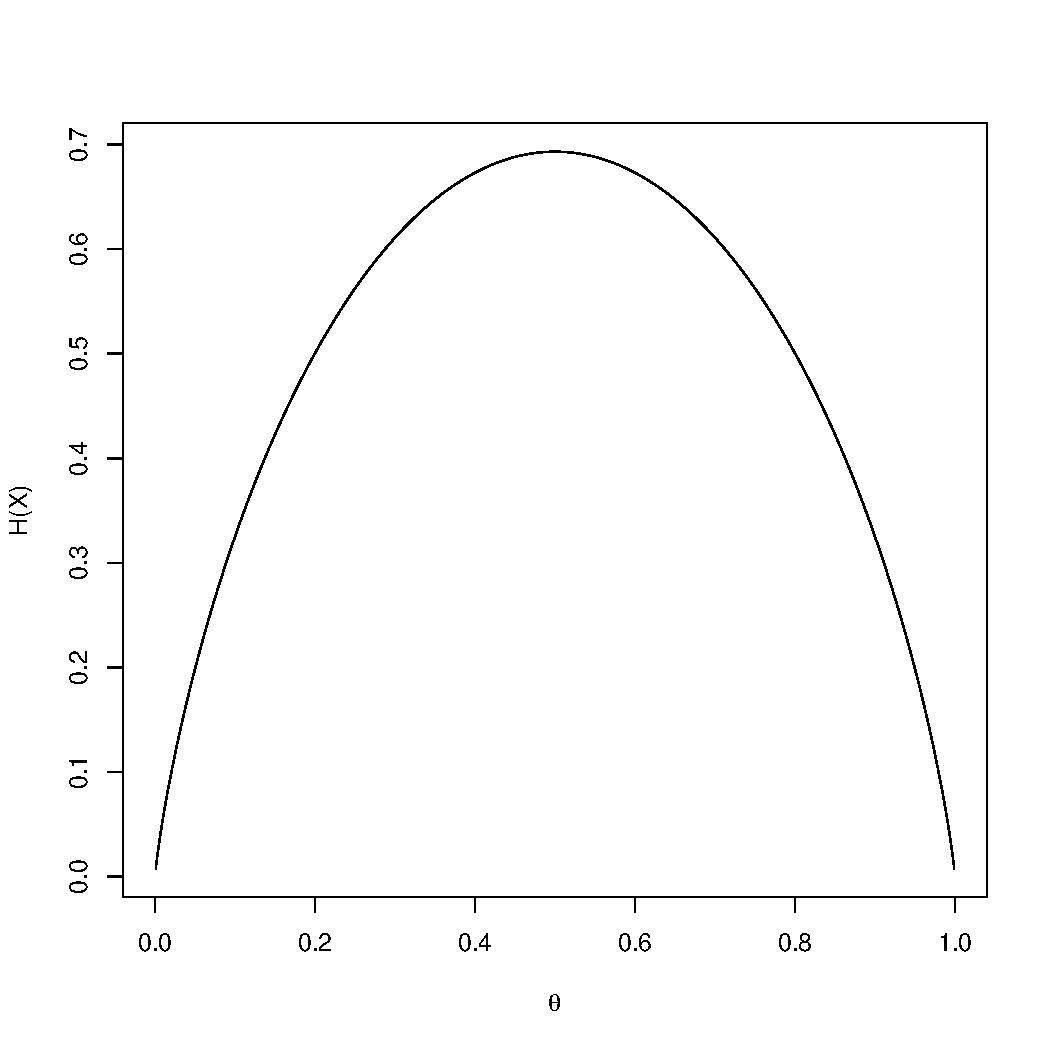
\includegraphics[width=\maxwidth]{figure/binaryEntropy-1} 

}

\caption[Binary entropy function]{Binary entropy function}\label{fig:binaryEntropy}
\end{figure}


\end{knitrout}

From the plot is it also easy to see that entropy is never negative. It holds in general that entropy is non-negative,
because entropy is defined as expectation of surprisal and surprisal is the negative logarithm of probabilities. 
Because $ \log(x) \leq 0 $ for $ x \in (0,1] $, it is clear that $ -\log(x) \geq 0 $ for $ x $ in the same
interval. Notice that from here on we drop the subscript and by convention let $ \log = \log_{2} $.

A standard interpretation of the entropy is that it quantifies uncertainty. As we have pointed out before, a uniform distribution means that you are most uncertain and indeed the uniform distribution maximizes the entropy. However, the more choices you have to pick from uniformly, the more uncertain you are going to be.  The entropy function also captures this intuition. Notice that if a discrete distribution is uniform, all probabilities are $ \frac{1}{|\supp(X)|} $. Clearly, as we increase $ |\supp(X)| $, we decrease the probabilities. By decreasing the probabilities, we increase their negative logarithms, and hence their average surprisal. Let us make this intuition more formal.

\begin{Theorem}
A discrete RV $ X $ with uniform distribution and support of size $ n $ has entropy
$ H(X) = \log(n) $.
\end{Theorem}

\paragraph{Proof:}
\begin{align}
H(X) &= \underset{x \in \supp(X)}{\sum}-\log(P(X=x))P(X=x) \\
&= \underset{x \in \supp(X)}{\sum} -\log(\frac{1}{|\supp(X)|})P(X=x) \\
&= \underset{x \in \supp(X)}{\sum}\log(n)P(X=x) = \log(n) \, .
\hspace{1cm} \square
\end{align}

\begin{Exercise}
You are trying to learn chess and you start by studying where chess grandmasters move their king when it
is positioned in one of the middle fields of the board. The king can move to any of the adjoining 8 fields. Since
you do not know a thing about chess yet, you assume that each move is equally probable. In this situation,
what is the entropy of moving the king?
\end{Exercise}

\section{Conditional Entropy}
At the outset of this section we promised you that you could easily transfer results from probability 
theory to information theory. We will not be able to show any kind of linearity for entropy because it contains
log-terms and the logarithm is not linear. We can however find alternative expressions for joint entropy (where 
the joint entropy is simply the entropy of a joint RV). Before we do so, let us also define the notion of 
conditional entropy. We have seen in Section~\ref{sec:jointconditionaldistributions} that $P_{X|Y=y}$ is a valid probability distribution for any $y \in \supp(Y)$ such that $P(Y=y)>0$. Hence, we can also define its conditional entropy.

\begin{Definition}[Conditional Entropy]
For two jointly distributed RVs $ X,Y $ and $y \in \supp(Y)$ such that $P(Y=y)>0$, the conditional entropy of $ X $ given that $ Y=y $ is defined as
\begin{align*}
H(X | Y=y) &:= \E_X[-\log_{2}(P(X=x | Y=y))] \\
&= - \!\! \sum_{x \in \supp(X)} P(X=x | Y=y) \log_2(P(X=x | Y=y))\, . 
\end{align*}
The conditional entropy of $X$ given $Y$ is defined as
$$ H(X | Y) := \E_Y[ H(X | Y) ] = \sum_{y \in \supp(Y)} P(Y=y) H(X | Y=y) \, .$$
\end{Definition}

Intuitively, $H(X | Y)$ is the (average) uncertainty of $X$ after learning $Y$. Intuitively, learning $Y$ (and in fact any information) cannot increase your uncertainty about $X$. Formally, one can prove the following 
\begin{Lemma}[see e.g.\ Proposition~4 of \href{http://homepages.cwi.nl/~schaffne/courses/inftheory/2016/notes/CramerFehr.pdf}{this script}] \label{lemma:noincrease}
For any two random variables $X,Y$ with joint distribution $P_{XY}$, it holds that $H(X | Y) \leq H(X)$.
\end{Lemma}
Note however, that this non-increase of uncertainty only holds on average, as illustrated by the following example:

\paragraph{Example}
Consider the binary random variables $X$ and $Y$, with joint distribution
\begin{align*}
&P(X=0,Y=0) = \frac{1}{2}, \quad P(X=0,Y=1) = \frac{1}{4}\\
&P(X=1,Y=0) = 0, \quad P(X=1,Y=1) = \frac{1}{4}.
\end{align*}
By marginalization, we find that $P(X=0) = \frac{3}{4}$ and $P(X=1) = \frac{1}{4}$, while $P(Y=0) = P(Y=1) = \frac{1}{2}$. This allows us to make the following computations:
\begin{align*}
H(X,Y) &= \frac{1}{2}\log 2 + \frac{1}{4} \log 4  + \frac{1}{4} \log 4 = \frac{3}{2}\\
H(X) &= h\left(\frac{1}{4}\right) = h\left(\frac{3}{4}\right) \approx 0.81\\
H(Y) &= h\left(\frac{1}{2}\right) = 1\\
H(X|Y) &= P(Y=0) \cdot H(X | Y=0) + P(Y=1) \cdot H(X | Y=1)\\
&= \frac{1}{2} \cdot 0 + \frac12 \cdot 1 = \frac12 \\
H(Y|X) &= P(X=0) \cdot H(Y | X=0) + P(X=1) \cdot H(Y | X=1)\\
&= \frac{3}{4} \cdot h\left(\frac{1}{3} \right) + \frac{1}{4} \cdot 0 \approx 0.69
\end{align*}
% We also could have computed $H(X|Y)$ and $H(Y|X)$ directly through the definition of conditional entropy.
Note that for this specific distribution, learning the outcome $Y=1$ increases the uncertainty about $X$, $H(X|Y=1) > H(X)$, but on average, we always have $H(X|Y) \leq H(X)$. It is important to remember that Lemma~\ref{lemma:noincrease} only holds on average, not for specific values of $Y$. Note also that in this example, $H(X|Y) \neq H(Y|X)$. 

It is not a coincidence that the joint entropy $H(X,Y)$ in the example above is equal to $H(X|Y)+H(Y)$ and $H(Y|X)+H(X)$. One can prove this chain rule in general:

\begin{align*}
H(X,Y) &= \underset{\substack{x \in \supp(X)\\y \in \supp(Y)}}{\sum} -\log(P(X=x,Y=y)) \times P(X=x, Y=y) \\
\begin{split}
&= \underset{\substack{x \in \supp(X)\\ y \in \supp(Y)}}{\sum} -\log(P(X=x \mid  Y=y)) \times P(X=x,Y=y) \\ 
&\qquad - \underset{y \in \supp(Y)}{\sum}\log(P(Y=y)) \times \sum_{x \in \supp(X)} P(X=x,Y=y) 
\end{split} \\
\begin{split}
&=\sum_{y \in \supp(Y)} P(Y=y) \times \sum_{x \in \supp(X)} -\log(P(X=x \mid  Y=y)) \times P(X=x \mid Y=y) \\ &\qquad - \underset{y \in \supp(Y)}{\sum}\log(P(Y=y)) \times P(Y=y)
\end{split} \\
&= H(X | Y) + H(Y) \; .
\end{align*}

\begin{Exercise}
Prove that $ H(X,Y | Z) = H(X | Z) + H(Y | Z) $ if $ X \bot Y \mid Z $.
\end{Exercise}


\section{An Information-Theoretic View on EM}
Now that we have seen some information-theoretic concepts, you may be happy to hear that there is an information-theoretic interpretation
of EM. This interpretation helps us to get a better intuition for the algorithm. To formulate that interpretation we need
one more concept, however.

\begin{Definition}[Relative Entropy]
The relative entropy of RVs \\ $ X,Y $ with distributions $P_X, P_Y$ and $\supp(X) \subseteq \supp(Y) $ is defined as
$$ D(P_X||P_Y) := \sum_{x \in \supp(X)} P(X=x) \log \frac{P(X=x)}{P(Y=x)} \ . $$
If $ P(Y=x) = 0 $ for any $ x \in \supp(X) $ we define $ D(P_X||P_Y) = \infty $. As with entropy, we often abbreviate $D(P_X||P_Y)$ with  $D(X||Y)$.
\end{Definition}

The relative entropy is commonly known as \textbf{Kullback-Leibler (KL)} divergence. It measures the entropy of $ X $ as scaled to $ Y $. Intuitively,
it gives a measure of how ``far away'' $ P_{X} $ is from $ P_{Y} $. To
understand ``far away'', recall that entropy is a measure of
uncertainty. 
% The
% relative entropy measure the uncertainty that you have about $ P_{X} $ if you know $ P_{Y} $\chris{hard to see why at this point}.
This uncertainty is low if both distributions place most
of their mass on the same outcomes. Since $ \log(1) = 0 $ the relative entropy is 0 if $ P_{X} = P_{Y} $.

It is worthwhile to point out the difference between relative and conditional entropy. Conditional entropy is the average entropy of $ X $ given that you
know what value $ Y $ takes on. In the case of relative entropy you do not know the value of $ Y $, only its distribution.

\begin{Exercise}
Show that $ D(X,Y||Y) = H(X | Y) $. Furthermore show that $ D(X,Y||Y) = H(X) $ if $ X\bot Y $.
\end{Exercise}


Let us start by remembering why we need EM. We have a model that defines a joint distribution
over observed ($ x $) and latent data ($ z $). Such a model generally looks as follows:
\begin{equation}
P(X=x, Z=z  \mid  \Theta = \theta) = P(X=x \mid Z=z, \Theta=\theta) P(Z=z \mid \Theta = \theta)
\end{equation}
where we have chosen a factorization that provides a separate term for a distribution over only the
latent data.

Recall that the goal of the EM algorithm is to iteratively increase the likelihood through consecutive
updates of parameter estimates. These updates are achieved through maximum-likelihood estimation based
on expected sufficient statistics. We are now going to show that a) EM computes a lower bound on the
marginal log-likelihood of the data in each iteration and b) that this lower bound becomes tight when the
expected sufficient statistics are taken with respect to the model posterior. The latter implies that
EM performs the optimal update in each iteration.

Let us start by expanding the data log-likelihood and then lower-bounding it.
\begin{align}
&\log(P(X=x \mid \Theta=\theta)) = \log(\sum_y P(X=x, Y=y \mid  \Theta = \theta))  \\
&= \log\left(\sum_{y} Q(Y=y \mid \Phi=\phi)\frac{P(X=x, Y=y \mid  \Theta = \theta)}{Q(Y=y \mid \Phi=\phi)}\right) \\
&\geq \sum_{y} Q(Y=y \mid \Phi=\phi) \log\left(\frac{P(X=x, Y=y \mid  \Theta = \theta)}{Q(Y=y \mid \Phi=\phi)}\right)
\label{eq:ELBO1}
\end{align}
Here, we have used \href{https://en.wikipedia.org/wiki/Jensen\%27s_inequality}{Jensen's Inequality} to
derive the lower bound. Observe that the log is indeed a concave function. 

We also have introduced
an auxiliary distribution $ Q $ over the latent variables with parameters $ \phi $. 
For reasons that we will explain shortly,
this distributions is often called the \textbf{variational distribution} and its parameters the
\textbf{variational parameters}. The letter $ Q $ is slightly non-standard to denote distributions but
we are are following conventions from the field of \textbf{variational inference} here.

In the next step, we factorise the model distribution in order to recover a KL divergence term between
the variational distribution and the model posterior over latent variables.
\begin{align}
&\sum_{y} Q(Y=y \mid \Phi=\phi) \log\left(\frac{P(X=x, Y=y \mid  \Theta = \theta)}{Q(Y=y \mid \Phi=\phi)}\right) \\
&= \sum_{y} Q(Y=y \mid \Phi=\phi) \log\left(\frac{P(Y=y \mid X=x, \Theta = \theta)P(X=x \mid \Theta = \theta)}{Q(Y=y \mid \Phi=\phi)}\right) \\
&= \sum_{y} Q(Y=y \mid \Phi=\phi) \log\left(\frac{P(Y=y \mid X=x, \Theta = \theta)}{Q(Y=y \mid \Phi=\phi)}\right) + \log(P(X=x \mid \Theta=\theta)) \\
&= -D(Q||P) + \log(P(X=x \mid \Theta=\theta)) \label{eq:ELBO2}
\end{align}
Equation~\eqref{eq:ELBO2} gives us two insights. First it quantifies the gap between the lower bound
and the actual data likelihood. This gap is equal to the KL divergence between the variational distribution
and the model posterior over latent variables. Second, since KL divergence is always positive, the bound only becomes
tight when $ P=Q $. But this is exactly what is happening in the E-step! The E-step sets $ P=Q $ and
then computes expectations under that distribution (see Equation~\eqref{eq:ELBO1}). Thus, the E-step increases
the lower bound on the marginal log-likelihood.

Looking back at Equation~\eqref{eq:ELBO1}, we also see that the M-step increases the lower bound because 
it maximises $ \E\left[P(X=x, Y=y\mid \Theta = \theta)\right] $. We conclude that both steps
are increasing the lower bound on the log-likelihood. We therefore conclude that EM increases the data likelihood
in every iteration (or leaves it unchanged at worst).

We will finish with a quick rejoinder on variational inference. EM is a special case of variational inference.
Variational inference is any inference procedure which uses an auxiliary distribution $ Q $ to compute
a lower bound on the likelihood. In the general setting, the auxiliary distribution can be different from the 
model posterior. This means that the bound never gets tight. However, in models in which the exact posterior 
is hard (read: impossible) to compute, using a non-tight lower bound instead can be incredibly useful!

The reason this inference procedure is called \textit{variational} is because it is based on the 
\href{https://en.wikipedia.org/wiki/Calculus_of_variations}{calculus of variations}. This works mostly
like normal calculus except that standard operations like differentiation are done with respect to functions
instead of variables.

%Naively, we could take the expectation with respect to any distribution
%over latent values. Obviously, we would like to find the best one, i.e. the one that is closest to the
%actual posterior. We can formalize this by introducing an auxiliary distribution\footnote{We follow
%standard notation here by denoting the auxiliary distribution $ Q $ instead of $ P $. Also, the
%parameter variable is chosen so as to distinguish it from the parameter variable of our model.} 
%$ Q(z\mid\Phi=\phi) $ under
%which we compute the expected sufficient statistics. We want to find the auxiliary distribution that
%is closest to actual posterior $ P_{Z\midX=x,\Theta=\theta} $. We measure closeness in an information-theoretic
%sense using KL-divergence. Formally, our goal is to find 
%\begin{equation}
%Q^{*}_{Z\mid\Phi=\phi} = \underset{Q_{Z\mid\Phi=\phi}}{\mbox{arg min}}~D\left( Q_{Z\mid\Phi=\phi} || P_{Z \mid X=x,\Theta=\theta} \right) \ .
%\end{equation}



\section*{Further Material}

At the ILLC, there is a whole course about information theory, \href{http://homepages.cwi.nl/~schaffne/courses/inftheory/}{currently taught by Christian Schaffner}. David MacKay also offers \href{http://www.inference.phy.cam.ac.uk/itprnn/book.pdf}{a free book on the subject}. Finally,
Coursera also offers \href{https://www.coursera.org/course/informationtheory}{an online course on information theory}.

The information-theoretic formulation of EM was pioneered in this \href{http://www.cs.toronto.edu/~fritz/absps/emk.pdf}{paper}. A very recent and intelligible 
\href{https://arxiv.org/abs/1601.00670}{tutorial on variational inference} can be found on the archive.

\end{document}

%%% Local Variables:
%%% mode: latex
%%% TeX-master: "chapter7"
%%% End:


\end{document}
